\chapter{Theory \label{ch:theory}}

\section{Introduction}

It is the goal of this section to succinctly derive some of the 
principal aspects of the Standard Model of particle physics and discuss the fundamental assumptions 
that give structure to the theory. Starting from classical physics how do we build up to an
 interacting theory of quantum theory of fields with the particle content of the Standard Model? 
What are the guiding principles of this model? And importantly what pieces of the theory have been put in by
hand to agree to experiment?

First, we will describe the Lagrangian formulation of classical mechanics. From here we introduce, 
classical field theory and the fundamental quantization of quantum mechanics to arrive at quantum field
theory (QFT). By way of Lagrangian symmetries in a QFT, we will elaborate on
gauge theories and how local gauge symmetries give rise to the interactions mediating the 
fundamental forces. We will review spontaneous electroweak symmetry breaking (EWSB) and the tools
 used to calculate scattering amplitudes. Ultimately, we will discuss radiative corrections, renormalization 
and Supersymmetry as an extension of the Standard Model. 

%% \begin{itemize}
%% \item Energy and The Principle of Minimal Action: Here we will build up the concept
%% \item Symmetry and Local Gauge Symmetry: What symmetries do we enforce upon the form of our theory
%% and what are the consequences.
%% \item Theory Renormalizability: What limits the type of terms we can include in our lagrangian as to preserve
%% the ability to calculate the outcomes of  scattering processes. 
%% \end{itemize}

\subsection{Quantum Field Theory}

\subsubsection{Lagrangian Mechanics}

In Lagrangian mechanics, the time evolution of some generalized coordinate $q$ can
be determined via the fundamental principle of minimal action for $\delta S = 0$ where $S=\int dt L$. Where the Lagrangian $L$ is difference between
 the kinetic and potential energy $T-V$. 
\begin{align*}
S[q(t)] &= \int_{t_1}^{t_2} L \left(q,\frac{dq}{dt},t\right) dt
\end{align*}
where $S$ is a functional of the time dependent generalized coordinate $q(t)$. 
Letting $\dot{q} = \frac{dq}{dt}$ The equations of motion are derived by varying S
\begin{align*}
\delta S &= \int_{t_0}^{t_1} \left [ \frac{\partial L}{\partial \dot q}  \delta \dot q + \frac{\partial L}{\partial q} \delta q \right ]dt 
\end{align*}
Note that $\delta \dot q = \delta\frac{dq}{dt} = \frac{d(\delta q)}{dt}$. 
Integrate the first term by parts, and require that $\delta q$ vanish at the boundaries:
\begin{align*}
\int_{t_0}^{t_1} \left [-\frac{d}{dt}\left (\frac{\partial L}{\partial \dot q} \right) \delta q + \frac{\partial L}{\partial q} \delta q \right ] dt  = \delta S = 0
\end{align*}
by the principle of minimal action we have arrived at the Euler equations of motion:
\begin{align*}
\frac{d}{dt}\left (\frac{\partial L}{\partial \dot q} \right) = \frac{\partial L}{\partial q}  
\end{align*}
For a generic Lagrangian with potential energy term $V(q)$, $L=\frac{1}{2}m_q \dot q^{2} - V(q)$  we obtain
the classical equation of motion as a differential equation $m\ddot{q}=-dV/dq$ that is $F=-dV/dq$.
\subsubsection{Classical Field Theory}
In comparison with classical mechanics, which deals with finitely many  general
 coordinates $q_i$, classical field theory deals with an infinite number of degrees of freedom 
$\phi_i(\vec x, t)$ with a degree of freedom for each spatial coordinate  $\vec x,t$ and 
index $i$. For simplicity we use a single index $\mu$ for the four space-time dimensions and utilize
the Einstein summation convention where repeated indices are summed over $x_ix_i \equiv \sum_i x_i x_i$. 
The corresponding action can be written in terms of a lagrangian density $\mathcal{L}(\phi,\partial_\mu \phi)$ \cite{tong}
\begin{align*}
S = \int dt L = \int d^3x \int dt \mathcal{L}(\phi,\partial_\mu \phi) = \int dx^4 \mathcal{L}(\phi,\partial_\mu \phi)
\end{align*}
Similarly, we arrive at classical Euler-Lagrange equations of motion:
\begin{align*}
\partial_\mu \left( \frac{\partial\mathcal{L}}{\partial (\partial_\mu \phi)}\right) = \frac{\partial \mathcal{L}}{\partial\phi}
\end{align*}
We now consider the simple free Lagrangian density for a real scalar field $\phi$:
\begin{align*}
\mathcal{L} = \frac{1}{2}(\partial_\mu \phi)^2 - \frac{1}{2} m^2\phi^2 =  \frac{1}{2}(\partial_t^2 - \nabla^2) \phi - \frac{1}{2} m^2\phi^2 
\end{align*}
we have achieved a relativistically invariance for free as all indices are contracted. To see this, consider a Lorentz transformation $\Lambda$ on the kinetic term. The transformation induces $\phi(x) \rightarrow \phi'(x) = \phi(\Lambda^{-1} x) = \phi (y)$. The transformation is $\Lambda$ as we actively
rotate the coordinate system rather than rotating the field. 
\begin{align*} 
\partial^\mu \partial_\mu  = \eta_{\mu\nu} \partial^\nu \partial^\mu \rightarrow_\Lambda \eta_{\mu\nu} (\Lambda^{-1})^\mu{}_\rho 
(\Lambda^{-1})^\nu{}_\sigma \partial^\rho \partial^\sigma  =  \eta_{\rho\sigma} \partial^\rho \partial^\sigma = \partial_\mu \partial^\mu 
\end{align*}
where we have used invariance of the spacetime metric under Lorentz transformations.
As the action integrates over all space time, the change of variable from $x\rightarrow y$ is
inconsequential and yield the same equations of  motion.
Applying the Euler-Lagrange equation we arrive at the 
classical relativistically invariant Klein-Gordon equation. 
\begin{align*}
(\partial^2 + m^2 ) \phi = 0
\end{align*}
taking the Fourier transform of state $\phi$:
\begin{align*}
\phi(\vec x, t) = \int \frac{d^3p}{(2\pi)^3} e^{i \vec p \cdot \vec x } \phi (\vec p, t)
\end{align*}
Where the $(2\pi)^3$ is a normalization convention on the field.  Applying the Klein Gordon equation 
\begin{align*}
( \partial^2 + m^2 ) \phi(\vec p, t)  = ( \partial_t^2   +  \vec{p}^2 + m^2)  \phi(\vec p, t) = 0 
\end{align*}
In this form, we recognize that this is just the equation of motion for a harmonic oscillator, $\partial_t^2 \phi = -\omega^2 \phi$
 with energy $\omega^2 = (\vec{p})^2 + m^2$.

\subsubsection{The Canonical Quantization}

Quantum mechanics consists of four fundamental postulates. Here we enumerate the postulates and their classical counter parts \cite{shankar}:
\begin{enumerate}
\item \textbf{Particle State}: In classical mechanics, a the state of a particle is determined by two variables $x(t)$ and $p(t)$. In quantum mechanics, the state is a vector $|\psi \rangle$ in a Hilbert space $\mathcal{H}$.
\item \textbf{Dynamic Variables }: Classically, all dynamical variables are a
 function only $x(t)$ and $p(t)$. In quantum mechanics, classical variables 
represented as a function of $x$ and $p$ are instead 
represented by Hermitian operators $X$ and $P$ that satisfy the commutation 
relation $[X,P] = XP - PX = i/\hbar$. 
\item \textbf{Measurement}: Classically, the particle state is unaffected by measurement and strictly
deterministic based on the values of $x$ and $p$. Quantum mechanically, a particle in a state $|\psi \rangle$ when measured will yield and eigenvalue $\omega$ of the operator $\Omega$ with probability
$|\langle\omega|\psi \rangle|^2$. After measurement, the particle state is in the corresponding eigenvector  $|\omega\rangle$.
\item \textbf{Time Evolution}: Classically, $p$ and $x$ change with time according to Hamilton's (or Lagrangian) equations of motion. Quantum mechanics asserts the state vector evolves with time according to the
Schr\"odinger equation: $i \hbar \frac{d}{dt}|\psi(t) \rangle = H | \psi(t) \rangle$. Where $H$ is the 
Hamiltonian with classical $p$ and $q$ replaced by the corresponding quantum mechanical operators.
\end{enumerate}

The canonical quantization arrises because the position and momentum operators no longer not commute (postulate 2). 
This is the source of the famous Heisenberg uncertainty principle that there are no simultaneously measurable states of $p$ and $q$. 

If we consider the quantum harmonic oscillator with Hamiltonian:
\begin{align*}
H = \frac{p^2}{2} + \frac{1}{2}\omega^2 q^2
\end{align*}
and define the creation ($a^\dagger$) and annihilation ($a$) operators
\begin{align*}
a = \sqrt{\frac{\omega}{2}}q + \frac{1}{\sqrt{2\omega}}p \text{ and   } a^\dagger = \sqrt{\frac{\omega}{2}}q - \frac{1}{\sqrt{2\omega}}p 
\end{align*}
we can re-write the position and momentum operators in terms of these operators:
\begin{align*}
q = \frac{1}{\sqrt{2\omega}} (a + a^\dagger) \text{ and } p = -i \frac{\omega}{2}( a - a^\dagger) 
\end{align*}
substituting into the Hamiltonian we find a simple solution after applying
the commutation relation $[p,q]=-i$ (using units where $\hbar=1$):
\begin{align*}
H = \left (a^\dagger a + \frac{1}{2} \right)  \omega
\end{align*}
Consequently the operations $[H,a]|E\rangle = (E-\omega)a|E\rangle$ and 
$[H,a^\dagger]|E\rangle = (E+\omega)a^\dagger|E\rangle$ show that the operators raise and 
lower the energy of the harmonic oscillator in multiples of $\omega$. The energy levels are quantized (i.e. 
restricted) to integer units of $\omega$. $a$ and $a^\dagger$ are also referred to as ladder operators,
as they raise and lower the energy state by 1 unit of $\omega$ with a non zero ground
 state energy $\omega / 2$. 

We can build a quantum field by promoting the coordinate $q$ to a field $\phi$ in the same
way as the classical field theory. This step is often referred to by a misleading name:
``the second quantization'', however there is only a single quantization in
the theory (the quantum quantization). We now write the solution to the Klein-Gordon
equation as an infinite sum of creation and annihilation operators that create 
or destroy a particle with energy $\omega_p^2 = p^2 + m^2$ designated by its four-momentum 
$p$. Taking the Fourier transform:
\begin{align*}
\phi(\vec x,t) = \int \frac{d^3p}{\sqrt{2\omega_{p}}} \left [  a_p e^{ipx} + a_p^\dagger e^{-ipx} \right ]
\end{align*} 
Quantum fields allow us to account for the observed phenomenon that particles are created and destroyed. 
Physical law is stated in terms of fields with infinite degrees of freedom that describe particles as excitations 
at points in space time. Ultimately, this will allow us to describe interactions occurring through
 virtual particles that are created and destroyed, but never observed. These kinematically unconstrained effects 
are a departure from the typical study of quantum systems with finite degrees of freedom. 

Although the above result only applies for a real scalar field (spin 0), the corresponding fermionic field (spin-$\frac{1}{2}$) field can be found similarly starting from the Dirac equation but now includes spinors. Written
in momentum space
\begin{align*}
\psi = \sum_s \int \frac{d^3k}{(2\pi)^32E_p} \left [ u(s,p)  a_{s,p} e^{-ikx} + v(s,p)a_{s,p}^\dagger e^{ikx} \right ]\\
\bar \psi = \sum_s \int \frac{d^3k}{(2\pi)^32E_p} \left[ \bar{v}(s,p) a_{s,p}  e^{-ikx} + \bar{u}(s,p)a_{s,p}^\dagger e^{ikx}\right]
\end{align*}
where the sum is taken over spin polarizations $s$ and $u,v,\bar{u},\bar{v}$ are dirac 
four-spinors which satisfy the completeness relationships with 
\begin{align*}
\sum_s u \bar{u} = p^\mu \gamma_\mu + m \\
\sum_s v \bar{v} = p^\mu \gamma_\mu - m
\end{align*}
Here, the gamma matrices $\gamma^\mu$ satisfy the anti-commutation relationships
$\{ \gamma^\mu, \gamma^\nu \} =  \gamma^\mu \gamma^\nu + \gamma^\nu \gamma^\mu = 2\eta^{\mu\nu}$.
The creation and annihilation operators now create states with a spin and momentum.

\subsection{Symmetries}
\textbf{Noether's Theorem}

The importance and the consequences of symmetries cannot be understated in physics. The
invariance of the action (equivalently the equations of motion) under linear translations of the  coordinates
gives rise to conservation of momentum. Similarly,  rotations of the coordinate space
yields the conservation of angular momentum. This is a consequence of Noether's theorem, that every 
continuous symmetry of the action has a corresponding conservation law. 

To be concrete, let us consider an action that is invariant under some field transformation
 $\phi \rightarrow \phi + \delta \phi$. If we consider a gauge transformation $\phi \rightarrow e^{i \beta}\phi$  
then the infinitesimal transformation is $\delta \phi = i \beta \phi$, here we assume the principle of
minimal action ($\delta S =0$) under this variation. This is the same as $\delta \mathcal{L}$ up to surface terms in the action integral. 
\begin{align*}
\delta \mathcal{L} &=  \left [ \frac{\partial \mathcal{L}}{\partial \phi} \delta \phi  + \frac{\delta \mathcal{L}}{\partial_\mu (\partial_\mu \phi)} \delta(\partial_\mu \phi) \right] =
 i\beta \left [ \frac{\partial \mathcal{L}}{\partial \phi}  \phi  + \frac{\partial \mathcal{L}}{\partial (\partial_\mu\phi)} (\partial_\mu \phi) \right]
\end{align*}
We further require that the solution satisfying the Euler-Lagrange equations, and exchange the first term:
\begin{align*}
&= i\beta \left [ \partial_\mu\left [ \frac{\partial \mathcal{L}}{\partial(\partial_\mu \phi)} \right ]  \phi  + \frac{\partial \mathcal{L}}{\partial_\mu \phi} (\partial_\mu \phi) \right] = i\beta \left [ \partial_\mu  \left [  \frac{\partial \mathcal{L}}{\partial(\partial_\mu \phi)}   \phi  \right ] \right ] = \partial_\mu \left [ \frac{\partial \mathcal{L}}{\partial (\partial_\mu \phi) }\right ] = \partial_\mu j^\mu 
\end{align*}
Where $j^\mu$  is the conserved current corresponding to the continuous symmetry. Accordingly minimal action tells us $\delta \mathcal{L} = 0 = \partial_\mu j^\mu$. 
 Now consider the consequences for fermonic Lagrangian:
\begin{align*}
\mathcal{L} = \bar{\psi}(i \gamma^\mu \partial_\mu -m)\psi
\end{align*}
the corresponding current is $j^\mu = i\bar \psi \gamma^\mu \psi = (\rho, \vec j)$ where $\rho$ is charge density and $\vec j$ is electric current.
When we expand the index and $\partial_\mu = (\frac{d}{dt}, \vec \nabla)$ we obtain the continuity equation:
\begin{align*}
\frac{d\rho}{dt} + \nabla \cdot \vec j = 0
\end{align*}
This corresponds to the conservation of charge. The change in the charge density of the system is equal to the outflowing current.
 It is critical to the study of particle physics that we understand the consequences of symmetries of the Lagrangian under such transformations. 
 The following sub-section will discuss the concept of symmetry in finer detail.

\textbf{Symmetry Groups and Algebras} \cite{groups}

Describing symmetry mathematically requires the definition of groups. The study of groups is known as group
theory and it is a subfield of abstract algebra. A group
is an algebraic structure that consists of a set $G$ (eg. Integers) and a pairwise operation (eg. multiplication) 
$a\cdot b = c$ where $a,b, c\in G$. The group must also contain an identity $i \in G$ (ex. 1) such that $i\cdot g = g$ for all $g\in G$.
All elements $g\in G$ must have an inverse $g^{-1} \in G$ such that $g \cdot g^{-1} = g^{-1} g = i$. The operation must 
additionally satisfy associativity $(a\cdot b) \cdot c = a \cdot (b \cdot c)$. The group does not necessarily
need to be commute $a\cdot b = b \cdot a$, a common example in physics is matrix multiplication. $M_{ij}N_{jk} \neq N_{ij}M_{jk}$ 
for all matrices $M$ and $N$. 

We can check the group of rotations $SO(3)$ (read special orthogonal group of
dimension 3) about the origin in euclidian $\mathbb{R}^3$ under composition for group like properties.
Clearly the composition of two rotations is another rotation, the inverse rotation is 
just rotating backward, and the identity is performing no rotation at all. 
The rotations can be represented by 3 by 3 matrices with real number valued element, determinant $\pm 1$, 
and inverses equal to their transpose $g^{-1}=g^T$. The group $SU(2) \cong SO(3) / \mathbb{Z}_2$, that is, $SU(2)$ is a double
 covering of $SO(3)$ corresponding to a redundancy of 2 elements $SU(2)$ for each element of $SO(3)$.

A lie group is a continuous group with a multiplicative 
law that is a differentiable function of the parameters. linear combinations of generator elements:
\begin{align*}
e^{-i\beta^i T^i} = U_{G}(\vec \beta)
\end{align*}
where the $T^i$ are the generator elements. 
For instance, we can build rotations in 3 dimensional space 
using the dimension 2 representation by exponentiating the Pauli spin matrices $\vec \sigma = (\sigma_1, \sigma_2, \sigma_3)$ 
with a conventional (1/2) normalization:
\begin{align*}
L_1 = \frac{\sigma_1}{2} = \frac{1}{2} \begin{pmatrix} 0 & 1 \\ 1 & 0 \end{pmatrix} \text{  }
L_2 = \frac{\sigma_2}{2} = \frac{1}{2} \begin{pmatrix} 0 & -i \\ i & 0 \end{pmatrix} \text{  } 
L_3 = \frac{\sigma_3}{2} =  \frac{1}{2} \begin{pmatrix} 1 & 0 \\ 0 & -1 \end{pmatrix} 
\end{align*}
A lie algebra of a group $G$ is defined by the commutation relations of its generators $T^i$, 
specifically:
\begin{align*}
[T^i, T^j] = T^iT^j - T^jT^i=  i c_{ijk} T^k
\end{align*}
where $c_{ijk}$ are the structure constants of the algebra. The algebra is abelian 
if and only if all $c_{ijk}=0$. Otherwise, by construction the $c_{ijk}$ must be anti-symmetric
 in any of the two indices. 

The Poincar\'e symmetry group $SO(3,1)$ (Lorentz transformations + translations) is the source  of the most fundamental conservation laws 
and the statistics of the quantum fields. A  transformation of the space-time coordinate $x^\mu$ takes the form:
\begin{align*}
x^\mu \rightarrow \lambda^\mu{}_\nu x^\nu + a^\mu 
\end{align*}
where $\Lambda^\mu_{}\nu$ is a transformation from the Lorentz group $SO(3,1)$ (boosts and rotations) and 
$a_\mu$ is a translation consisting of single 4-vector $\mathbb{R}^{3,1}$. 

The generators of the Poincar\'e group can be enumerated as generalized angular momentum operators:
$M_{\mu\nu} = i(x_\mu \partial_\nu - x_\nu \partial_\mu)$ with the commutation relations:
\begin{align*}
[M_{\mu\nu}, M_{\rho\sigma}] = -i(\eta_{\mu\rho} M_{\nu \sigma}  - \eta_{\nu \sigma} M_{\nu \rho} + 
\eta_{\nu \sigma} M_{\mu \rho} - \eta_{\nu \rho} M_{\mu \sigma})
\end{align*}
However, by decomposing the operators into rotations and boosts these relations become much simpler. Define:
\begin{align*}
J_i = \frac{1}{2}\epsilon_{ijk} M_{jk} \text{  and   } P_i = i\partial_i \text{  and   } K_i = M_{0i}
\end{align*}
Where $J$ and $P$ are the familiar angular and linear momentum operators. The $K_i$ correspond to rapidity boosts. 
With this notation, we can derive more easily digested commutation relations:
\begin{align*}
[J_i, J_j] &= i \epsilon_{ijk}J_k  & [P_0,J_j] &= 0 \\
[P_i,J_j] &= i \epsilon_{ijk} P_k & [P_0, K_i] &= i P_i \\
[P_i,K_j] &= i P_0 \delta_{ij} & 
\end{align*}
For a given lie algebra, the dimension of the representation of the group is physically related to the 
quadratic Casimir. For a given concrete representation $L_n$ for a $n$ dimensional
representation, the quadratic Casimir $C_2$ can be written as:
\begin{align*}
L_n^2 = C_2(L_n)I  \text{  and for example in SO(3) } J^2 = j(j+1) I
\end{align*}
where $I$ is the identity. In $SO(2)$ the $j$ representation
has dimension $n=2j+1$ with quadratic Casamir $j(j+1)$. For $j=0$ we have $n=1$ 
where the rotation is trivial and $J^2 =1$. For $j=1/2$, $J^2=\frac{3}{4}$ and $n=2$.
%% \begin{align*}
%% L_1 = \begin{pmatrix} 0 & 0 & 0 \\ 0 & 0 & -i \\ 0 & i & 0 \end{pmatrix} \text{   } L_2 = \begin{pmatrix} 0 & 0 & i \\ 0 & 0 & 0 \\ -i & 0 & 0 \end{pmatrix} \text{   } L_3 = \begin{pmatrix} 0 & -i & 0 \\ i & 0 & 0 \\ 0 & 0 & 0 \end{pmatrix}
%% \end{align*}
The Lorentz group can further be decomposed into  $SO(3,1) \cong SU(2) \times SU(2)$
where $SU(2)$ is the group of matrices with determinant $\pm 1$ where the inverses are
 the conjugate transpose: $g^{-1} = (g^{T})^*$. The fundamental fields in the Standard Model
Lagrangian are characterized by the four corresponding combinations of $SU(2)$ representations. The (0,0) representation 
of $SU(2) \times SU(2)$ corresponds to scalar spin 0 fields $\phi$. The two chiral representations
 ($\frac{1}{2}$,0) and (0,$\frac{1}{2}$) correspond to fermionic matter fields $\psi$,$\bar{\psi}$. 
The ($\frac{1}{2}$,$\frac{1}{2}$) representation corresponds to the fundamental vector 
boson fields $W^i_\mu, B_\mu, G^i_\mu$ and the fields after
 EWSB. $W^{\pm}_\mu, Z^0_\mu, A_\mu, G^i_\mu$. 

There are three fundamental gauge groups which govern the Standard Model which also arise as symmetries in unrelated systems.
The first group, $U(1)$, governing electric hyper charge is simply unitary $1\times 1$ matrices i.e. complex numbers. The
second group in context of rotations in Euclidian space is $SU(2)$ governing the weak force. The group is generated
by the Pauli spin matrices plus the identity with structure constants $c_{ijk} = \epsilon_{ijk}$. 
The final group $SU(3)$, the strong force gauge group, is similar in structure to $SU(2)$ and is generated
by the eight Gell-Man matrices ($\lambda_i$ for $i=1\ldots 8$) and the identity matrix.  The Gell-Mann matrices
are the three dimensional analogues to the Pauli spin matrices. Each matrix is traceless and satisfies the  
commutation relations with anti-symmetric structure constants $f_{ijk}$. 

Consider a field transformation $\phi_a \rightarrow \phi_a'$ under some lie algebra with
generators $L_i$ such that the transformation is $U_g(\beta)$. In the Heisenberg picture of quantum mechanics 
where operators evolve but the states remain fixed:
\begin{align*}
&\langle O' \rangle = \langle \phi | U_g^{-1}(\beta) O U_g(\beta) | \phi \rangle\\
\implies & O'= U_g^{-1}(\beta) O U_g(\beta)
\end{align*}
we obtain a transformed quantum field:
\begin{align*}
\phi_a' = e^{-i \vec \beta \cdot \vec T} \phi_a e^{i \vec \beta \cdot \vec T}
\end{align*}
the exponentials can be expanded as nested commutators 
\begin{align*}
\phi_a' = \phi_a - i [ \vec \beta \cdot \vec T, \phi_a] + \frac{(-i)^2}{2}[ \vec \beta \cdot \vec \tau, [ \vec \beta \cdot \vec T, \phi_a]] + O(\beta^2)
\end{align*}
If  $L^i$ is the concrete representation of $T^i$. applying the commutation relation
 $[T^i, \phi_a] = - L_{ab}^i \phi_b$ gives the field transformation law in terms of the representation:
\begin{align*}
\phi_a' = \left (e^{i \vec \beta \cdot \vec L} \right)_{ab} \phi_b 
\end{align*}
Similarly the conjugate field $\phi^\dagger_a$ transforms in the adjoint representation:
\begin{align*}
\phi_a^\dagger = \left( e^{-i \vec \beta \cdot \vec L} \right)_{ab} \phi^\dagger_b 
\end{align*}
\textbf{Local Gauge Invariance and the Covariant Derivative} \cite{peskin}

What if we promote the Lagrangian symmetry of fields under the Standard Model gauge symmetries to a local symmetry? The symmetry is local 
with a value dependent on the position in space-time $x^\mu$. For example, a local $U(1)$ gauge symmetry would transform the field $\psi$ as:
\begin{align*}
\psi(x) \rightarrow e^{i\alpha(x)} \psi(x)
\end{align*}
If we then consider a direction derivative in the direction $n^\mu$ as defined:
\begin{align*}
n^\mu \partial _\mu \psi (x) = \textrm{lim}_{\epsilon\rightarrow 0} \frac{\psi(x + \epsilon n) - \psi(x)}{\epsilon}
\end{align*}
This is not going to have a simple transformation law, since the two states are not at the same
point in space time. We need a connection $U(x,y)$ the  derivative transformations simply. Taking the directional derivative:
\begin{align*}
n^\mu \partial _\mu \psi (x) = lim_{\epsilon\rightarrow 0} \frac{1}{\epsilon} \left ( \psi(x + \epsilon n) - U(x+\epsilon n, x) \psi(x) \right)
\end{align*}
where $U(x,y)$ is our connection and transforms as:
\begin{align*}
U(x,y) \rightarrow e^{i\alpha(x)} U(x,y) e^{-i\alpha (y)}
\end{align*}
such that when we apply the transformation to the directional derivative we obtain:
\begin{align*}
n^\mu \partial _\mu \psi (x) = lim_{\epsilon\rightarrow 0} \frac{1}{\epsilon} e^{i\alpha(x+n\epsilon)} \left ( \psi(x + \epsilon n) - U(x+\epsilon n, x) \psi(x) \right)
\end{align*}
Now lets expand the transformation for an infinitesimal $\epsilon$:
\begin{align*}
U(x+\epsilon n, x) \approx U(x,x) + c\epsilon n^\mu A_\mu (x) + O(\epsilon^2)\\
= 1 + c\epsilon n^\mu A_\mu (x) + O(\epsilon^2)
\end{align*}
The connection between $x$ and itself was trivial and we have specified an arbitrary (while suggestive) constant $c = ie$.
If we would then like to see how this field $A_\mu$ transforms we need to check the $U(x,y)$ transformation:
\begin{align*}
e^{i\alpha(x)} U(x+\epsilon n,x) e^{-i\alpha (y)} &= (1 + i \alpha(x+n\epsilon)) (1-ie\epsilon n^\mu A_\mu)(1 - i \alpha x) \\
&= 1 + i \alpha (x+n\epsilon ) - ie \epsilon n^\mu A_\mu - i\alpha(x)
\end{align*}
comparing this to the expansion of $U(x+\epsilon n, x)$ we see:
\begin{align*}
1 + ie\epsilon n^\mu A_\mu (x) &\rightarrow 1 + i \alpha (x+n^\mu\epsilon ) - ie \epsilon n^\mu A_\mu(x) - i\alpha(x)\\
A_\mu(x) &\rightarrow  \left [ \frac{\alpha(x+n^\mu\epsilon) + \alpha(x)}{en^\mu \epsilon} + A_\mu(x) \right] \\
A_\mu(x) &\rightarrow  \left [  A_\mu(x)  -\frac{1}{n^\mu}\frac{1}{e}\partial_\mu \alpha(x) \right]
\end{align*}
If we pick the axes such that $n^\mu = 1$ then we have the transformation law for the gauge field: $A_\mu(x) \rightarrow A_\mu(x) - \frac{1}{e} \partial_\mu \alpha(x)$. 

Now that we understand how the field component must transform under a gauge transformation, apply a U(1) gauge transformation $U(\alpha)$ 
 to a field. It should be understood that $\alpha$ is now local.
\begin{align*}
\psi' = U(\alpha) \psi = ( e^{i\alpha})\psi \text{ and } \mathcal{L}' = U(\alpha)\psi \partial^\mu ( U(\alpha) \psi)
\end{align*}
because the transformation is local, the derivative will act on the transformation and an extra term is generated:
\begin{align*}
\partial^\mu ( U(\alpha) \psi) = U(\alpha) \partial^\mu \psi + ( \partial^\mu U(\alpha)) \psi 
\end{align*}
This term is not gauge invariant as the transformation appears explicitly. To account for this, we introduce a substitution for $\partial^\mu \rightarrow D^\mu $
which will allow us to preserve gauge invariance 
\begin{align*}
\partial^\mu \rightarrow D^\mu = \partial^\mu + igA^\mu
\end{align*}
Checking the transformation law for $\partial^\mu \psi\rightarrow D^\mu\psi$ with the necessary $A^\mu$ transformation included
\begin{align*}
(\partial^\mu + ig A^\mu ) \psi \rightarrow &\left (\partial^\mu + ig  (A^\mu +  \frac{1}{g} \partial^\mu \alpha)\right )( e^{-i \alpha } \psi ) \\
&= e^{-i \alpha } \partial^\mu \psi + ig A^\mu e^{-i\alpha} \psi - i\partial^\mu \alpha e^{-i \alpha} \psi + i\partial^\mu \alpha e^{-i \vec \alpha} \psi \\
&= e^{-i \alpha} (\partial^\mu + ig  A^\mu )\psi \\
&= U(\alpha) D^\mu \psi
\end{align*}
For non-abelian gauge groups, the introduction of the covariant derivative will enforce local 
gauge symmetry of the Lagrangian, but require modified substitutions
\begin{align*}
A^{\mu,i} &\rightarrow A^{\mu,i} -  c_{ijk} \alpha_j A^{\mu,k} - \frac{1}{g} \partial^\mu \alpha_iL^i\\
\partial^\mu &\rightarrow D^\mu =  \partial^\mu + igA_{\mu,i}L_i
\end{align*}
where $c_{ijk}$ are the structure constants, $A_i$ are the gauge bosons for the transformation, and $L_i$ are the 
concrete representations of the generators. 

The consequence of promoting the partial derivatives to gauge symmetry preserving covariant derivatives yields new terms in the Lagrangian
\begin{align*}
i\bar{\psi} \partial_\mu\gamma^\mu \psi  \rightarrow i\bar{\psi} \partial_\mu\gamma^\mu \psi - e\bar{\psi} A_\mu \gamma^\mu \bar{\psi}
\end{align*}
New gauge interactions with the matter fields have arisen. The force's symmetry group and the invariance of the Lagrangian
naturally induce the force's interactions with matter. Symmetries always always have important consequences to a 
theory. The following section will expand in detail the variety of terms in the Standard Model Lagrangian.

\subsection{The Standard Model Lagrangian}

The Standard model of particle physics is a quantum field theory of 3+1 dimensional 
spacetime governed by a Lagrangian with four sectors and three local gauge symmetries
developed to describe and study the physics of fundamental particles in the physical, observable universe.  
\begin{center}
\begin{table}[]
\begin{center}
\caption{Standard Model particle representations under the symmetry groups $SU(2)$ and $SU(3)$ respectively $n_2$ and $n_3$. Also listed is associated electroweak hyper charge $Y$ as well as the electric charge $Q$ }
\begin{tabular}{ccccccccc}
                & $q_L$ & $l_L$  & $u_R$ & $d_R$  & $e_R$ & $\nu_R$ & $\phi$ \\
\hline
$n_3$           & 3     & 1      & 3     & 3      & 1     & 1  & 1     \\
$n_2$           & 2     & 2      & 1     & 1      & 1     & 1  & 2     \\
$Y_{U(1)}$      & 1/6   & $-1/2$ & $2/3$ & $-1/3$ & $-1$  & 0  & 1/2     \\
\hline
\hline
$Q = Y + T_L^3$ & 2/3   & $-1$ & 2/3   & $-1/3$ & $-1$  & 0 & 0
\end{tabular}
\end{center}
\label{tab:charges} 
\end{table}
\end{center}
\begin{center}
\begin{table}[]
\begin{center}
\caption{cite-tully-particle: The fundamental fields types contained in the SM Lagrangian}
\begin{tabular}{ccc}
Field & Lagrangian Term & Field Dim. [Mass]\\
\hline
Scalar Field & $(1/2)(\partial_\mu \phi)(\partial^\mu \phi)$ & $[\phi]=M^2$\\
Dirac Field & $\bar \psi M \psi$  & $[\psi]=M^{3/2}$\\
Field Stress Tensor &$-(1/4)F_{\mu\nu}F^{\mu\nu}$ & $[F_{\mu\nu}]=M^2$ \\
Vector Field & $F_{\mu\nu} = \partial_\mu A_\nu - \partial_\nu A_\mu$ & $[A_\mu]=M$\\
\end{tabular}
\label{tab:fields}
\end{center}
\end{table}
\end{center}

\begin{center}
\begin{table}[]
\begin{center}
\caption{The types of terms included in the Standard Model Lagrangian \cite{tully}}
\begin{tabular}{ccc}
Coupling Type & Lagrangian Term &  Coupling Dim [Mass]\\
\hline
Scalar Coupling w/ Gauge Bosons & $\tilde{g} A_\mu A^\mu \phi$ & $[\tilde{g}] = M$ \\
& $g A_\mu(\partial^\mu \phi) \phi$ & $[g] =1$\\
Scalar self-couplings & $\tilde{g}\phi^3$ & $[\tilde{g}] = M$ \\
& $g \phi^4$ & $[g] = 1$ \\
Gauge Coupling & $g \bar \psi \gamma_\mu \psi A^\mu$ & $[g] = 1$ \\
Triple Gauge Coupling & $A_\mu A^\mu \partial_\nu A^\nu$ & $[g] = 1$ \\
Quartic Gauge Coupling & $g^2 (A_\mu A^\nu)^2$ & $[g] = 1$ \\
Yukawa Coupling & $g \bar \psi \psi \phi$ & $[g] = 1$ 
\end{tabular}
\label{tab:interactions}
\end{center}
\end{table}
\end{center}

\begin{center}
\begin{table}[]
\begin{center}
\caption{The 19 free parameters of the Standard Model with values as dictated by experimental observation}
\begin{tabular}{cccc}
\textbf{Category} & \textbf{Name} & \textbf{Parameter} & \textbf{Remarks} \\
\hline
Lepton Masses & Electron, Tau, and Mu  & $m_e,m_\mu,m_\tau$ & $m_l = (\lambda_l \nu)/2$ \\
Fermion Masses & Up, Charm, Top & $m_u, m_c, m_t$ & \\ 
   & Down, Strange, Bottom & $m_d, m_s, m_b$ & \\
\hline
CKM Matrix & Mass-Flavor Mixing Angles & $\theta_{12},\theta_{23},\theta_{13}$ & \\ 
 & CP Violating Phase  & $\delta$ & \\ 
\hline
Higgs Parameters & Vacuum Expectation Value &  $\nu$ & $\nu= \mu / \sqrt{\lambda}$   \\
& Higgs Mass & $m_{h}$ &   $m_h^2 = -2\mu^2$  \\
\hline
Force Strength & Gauge Couplings & $g, g', g_s$ & $\alpha, \alpha_w, \alpha_s$  \\ 
\hline
CP Violating Terms & Vaccum QCD Angle  & $\theta_{QCD}$ &  unobserved \\
\hline
\end{tabular}
\end{center}
\label{tab:free_params}
\end{table}
\end{center}
The Standard Model Lagrangian has three types of fundamental fields: spin-0 (scalar boson), spin-1/2 (dirac fermion), and spin 1 (vector boson). 
Any theory  describing gravity would also include a unique spin-2 particle mediating gravity known
as the graviton. A supersymmetric theory of gravity would also include a particle of spin-3/2,
a supersymmetric partner of the graviton known as the gravitino.  The complete field
content of the theory is listed in Table \ref{tab:fields} with the
associated mass dimensions of the fields. Dimensional analysis tells
us the mass dimension of the Lagrangian is 4 as dictated by the action being unitless. Requiring mass dimension
4 of each term (by dimensional analysis) and requiring that all indices are contracted (Lorentz invariance) 
is highly constraining to the types of terms within the Lagrangian. 
The types of interactions (after EWSB) are listed 
in Table \ref{tab:interactions}. 

It is important to understand the principal components of the theory, so we can separate
 the aspects which are emergent from the underlying assumptions and those which are put in
 by hand. Here we list principal aspects of the theory.

\begin{enumerate}
\item \textbf{Relativistic Theory:} The Lagrangian must be invariant under Lorentz transformations as well as rotations and translations in 3+1 dimensional spacetime. 
\item \textbf{Matter:} There are three families of fermonic particles consisting of an up-type 
quark with an associated down-type quark and a lepton with an associated neutrino.
\item \textbf{Fundamental Charges:} Each particle transforms as a multiplet of the gauge symmetries as dictated in Table 2.1. This  determines how the 3
 forces interact with matter. 
\item \textbf{Gauge Symmetry:} The fundamental action must be invariant under local gauge transformations.
\item \textbf{Free Parameters:} The Lagrangian includes 19 free parameters which set the experimentally observed fermion masses, interaction strengths, mass-flavor mixing, the vacuum potential and the possible charge parity symmetry violating terms in the strong sector
 (Table 2.4). 
\item \textbf{Renormalizable:} All terms of the Standard Model have been shown to be renormalizable. 
 This also means there are no terms with mass dimension greater than 4. Higher
 dimension terms have dimensions of inverse mass and are irrelevant until experiments are made
 capable of probing near the energy scale $\Lambda$ where the Standard Model theory breaks down.
\end{enumerate} 

The simplicity of the governing assumptions and naturalness of free parameters are certainly 
an ambition of any theory of fundamental particle physics, but a more aesthetically 
pleasing theory is not necessarily the ultimate goal. The Standard
Model, is a tool towards finding a more complete theory. The theory admits 
incompleteness in its formulation (eg. the exclusion of gravity), but achieves
incredible experimental verification \cite{gminus2} of theoretical predictions \cite{loop8qed} accurate to 14 decimal places where
the theory is tested. 

The Standard Model Lagrangian can be grouped into four sectors written in a simplified form where the individual terms have not been 
expanded and EWSB has yet not occurred: 
\begin{align*}
\mathcal{L}_{SM} &= \mathcal{L}_{Gauge} + \mathcal{L}_{Fermion} + \mathcal{L}_{Higgs} + \mathcal{L}_{Yukawa}\\
&=\left(-\frac{1}{4} F_{\mu\nu}F^{\mu\nu} \right )
  + \left (\bar\psi i\gamma^\mu \partial_\mu \psi \right) +
 \left(\frac{1}{2}(\partial_\mu \phi)^2 + V(\phi) \right) + \left(\bar \psi_i y_{ij} \psi_j \phi \right ) 
\end{align*}
In our discussion, we will expand each sector in terms of the field content and point out free parameters of the
theory where they have been included. 
\begin{figure}
\begin{center}
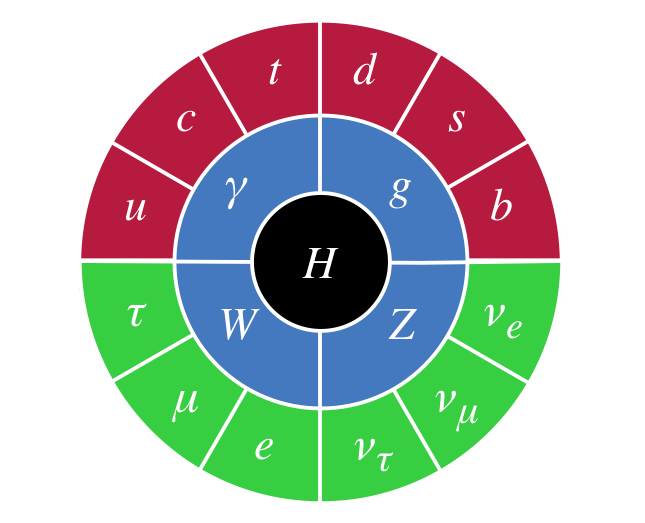
\includegraphics[width=.45\textwidth]{pics/sm_model_particles}
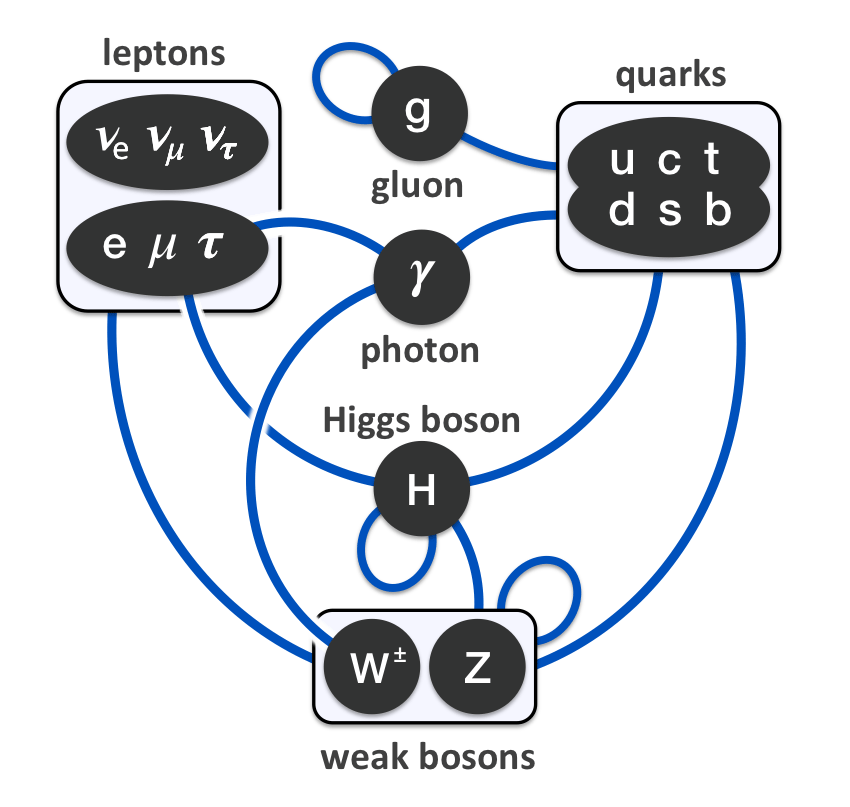
\includegraphics[width=.45\textwidth]{pics/principal_interactions}
\caption{ (left) A representation of the particle content of the Standard Model. 
The inner circle is the unique scalar Higgs field. The next ring consists of the 
gauge bosons. The outer ring are the fermonic fields broken into quarks and leptons. (right) Lines drawn between particles show the fundamental interaction terms in the theory. Higher order effects can generate interactions not shown here (such as $h\rightarrow \gamma\gamma$ which is generated through a top quark loop.}
\end{center}
\end{figure}

\subsubsection{Gauge Sector}

The gauge sector consists of the field stress energy tensor of the 3 corresponding types of gauge bosons:
 $G^i$ (gluons of the color force), $W^i$ ($W$'s of the weak force) and $B$ (of the weak hyper charge). Here the index $i$ enumerates their multiplicity. There are 8 gluons, 3 $W$'s and a single B. Ultimately, we will arrive have 8 gluons, $W^{\pm}$, $Z^0$, and the photon $A$ after the $SU(2)\times U(1)$ symmetry is spontaneously broken 
and the scalar field $\phi$ takes on a new vacuum state. The strong color force remains unbroken. 

Although not exclusive to this sector, the gauge transformations add three free parameters to the theory corresponding to the gauge
coupling strengths: $g$,$g'$, and $g_s$. 

\begin{equation}
\mathcal{L}_{Gauge} = - \frac{1}{4} F_{\mu\nu}^{i} F^{\mu\nu i} =  - \frac{1}{4} G_{\mu\nu}^{i} G^{\mu\nu i} - \frac{1}{4} W^{i}_{\mu\nu} W^{\mu\nu i} - \frac{1}{4} B_{\mu\nu}B^{\mu\nu} 
\end{equation}
where the double scripts correspond to the commutation relations for the gauge group algebra:
\begin{align*}
X_{\mu\nu}   &= [D_u X_\nu, D_\nu X_\mu] \\
[\partial_\mu X_\nu, \partial_\nu X_\mu ] &= \partial_\mu X_\nu - \partial_\nu X_\mu - g f_{ijk} X_\mu^j X_\nu^k
\end{align*}
where $g$ is the coupling constant, the $D_\mu$ terms correspond to the covariant derivative and the $f_{ijk}$ are the corresponding structure constants for the non-abelian groups that arise from the non commuting generators of the algebra. The $B_\mu$ has no structure constants, the $W^i$ of $SU(2)$ have $f_{ijk}=\epsilon_{ijk}$ and the $SU(3)$ has $f_{ijk}$ determined by 8 Gell-mann $\lambda_i$ generators.
%% \begin{align*}
%% G_{\mu\nu}^i &=  D_\mu G_\nu^i - D_\nu G_\mu^i - g_s f_{ijk} G_\mu^j G_\nu^k\\ 
%% W_{\mu\nu}^i &=  D_\mu W_\nu^i - D_\nu W_\mu^i - g \epsilon_{ijk} W_\mu^j W_\nu^k\\ 
%% B_{\mu\nu} &=  D_\mu B_\nu - D_\nu B_\mu
%% \end{align*}
After EWSB, when these terms are written in  the mass eigenstates of the theory, this sector generates self-interactions 
between  gauge bosons such as the triple and quartic gauge couplings as shown in Table \ref{tab:interactions}. 

\subsubsection{Fermion Sector}

The fermion sector consists of the kinetic energy terms for each quark (up and down types) and leptons (lepton, neutrinos) in the Standard Model.
The left handed quarks transform as an $SU(2)$ doublet:
\begin{equation}
q_{m\alpha}^L = \left( \begin{array}{c} u_{m\alpha}  \\ d_{m\alpha} \end{array} \right)^L \text{ and } l_{m}^L = \left( \begin{array}{c} \nu_{m}  \\ e^{-}_{m} \end{array} \right)^L 
\end{equation}
where the subscript $m$ denotes the family (1st, 2nd and 3rd generation) and $\alpha$ denotes the color charge (red, green, and blue).
As the $SU(2)_L$ symmetry only acts on the left handed fermions we further separate the fermion sector into left and right components:
\begin{align*}
\mathcal{L}_{fermion,L} &= \bar{q}_{mL} i \gamma^\mu D_\mu q_{mL} + \bar{l}_{mL} i \gamma^\mu D_\mu l_{mL}\\
\mathcal{L}_{fermion,R} &=  \bar{u}_{mR} i \gamma^\mu D_\mu u_{mR} 
+ \bar{d}_{mR} i \gamma^\mu D_\mu d_{mR} + \bar{e}_{mR} i \gamma^\mu D_\mu e_{mR} + \bar{\nu}_{mR} i \gamma^\mu D_\mu \nu_{mR}
\end{align*}

\subsubsection{Yukawa Sector}

The Yukawa sector consists of couplings  between the matter fields and the scalar field $\phi$.
\begin{align*}
\mathcal{L}_{Yukawa} = - \sum_{m,n=1}^3 \left [ y^u_{mn} \bar{q}_{mL} \tilde{\phi} u_{nR} + y^d_{mn} \bar{q}_{mL} \phi d_{nR}  + y_{mn}^e \bar{l}_{mL} \phi  e_{nR}  \right ] + (h.c) 
\end{align*}
The sum is taken over families $n,m$. The single scalar field $\phi$ is written in two ways: $\phi = ( \phi^+ , \phi^0)$ and $\phi$ after
a $SU(2)$ gauge transformation $\tilde{\phi} = i \tau^2 \phi^\dagger = \epsilon \phi^\dagger = 
(\phi^\dagger , -\phi^-)$. These terms need to be included such that we will
 later be able to generate mass terms for the up type quarks during EWSB. The reason
we would not able to write these terms is they would violate weak hyper charge gauge invariance.  Similarly, 
we can not write explicit mass terms $\bar{u}_Lm u_R + (h.c.)$ since the left and right particles have
different hyper charge. To be concrete calculate the total hyper charge:
\begin{align*}
\bar{q}_{mL} \phi u_{nR} \implies Y= -\frac{1}{6} + \frac{1}{2} + \frac{2}{3} = 1 \neq 0
\end{align*}
Whereas $\tilde{\phi}$ will transform in the adjoint representation:
\begin{align*}
\bar{q}_{mL} \tilde{\phi} u_{nR} \implies Y= -\frac{1}{6} - \frac{1}{2} + \frac{2}{3} = 0
\end{align*}
The Yukawa sector  contains a large number of the free parameters in the Standard Model (13 of 19). 
The individual masses of each fermion and lepton are generated by the $y_{ij}$
terms which are set to agree with experimental values (9 free parameters). These parameters 
also set the coupling of the corresponding interaction strength with the Higgs boson after electroweak symmetry
breaking.

The Yukawa couplings also also implicitly include parameters characterizing the mismatch 
mixing between the quark flavor and mass eigenstates that occurs after EWSB  (4 parameters). 
Had the mass flavor states been aligned, we would not need the two family indices to 
be able to generate mass terms after EWSB. The mixing is characterized by  the $3\times 3$ unitary
 Cabibbo-Kobayashi-Maskawa (CKM) matrix $V^{CKM}$. The convention is chosen that flavor
 states $u^I$ for up type quarks are aligned with the mass states $u$ with the down type quarks 
rotated by the transformation $d^I_i = V^{CKM}_{ij} d_{j}$. From the unitarity condition, the matrix can be
 parameterized in 4 parameters: three mixing angles $\theta_{12}, \theta_{23}, \theta_{13}$ and a CP violating phase $\delta$:

\begin{align*}
\begin{pmatrix}  d^I \\ s^I \\ b^I \end{pmatrix} &=
 \begin{pmatrix} V_{ud} & V_{us} & V_{ub} \\ V_{cd} & V_{cs} & V_{cb} \\ V_{td} & V_{ts} & V_{tb} \end{pmatrix} 
\begin{pmatrix}  d \\ s \\ b \end{pmatrix}  \\
&= \begin{pmatrix} c_{12}c_{13} & s_{12} c_{13} & s_{13} e^{-i\delta} \\ 
-s_{12}c_{23} - c_{12}s_{23}s_{13}e^{i\delta} & c_{12} c_{23} - s_{12} s_{23} s_{13} e^{i\delta} & s_{23} c_{13} \\
s_{12}s_{23} - c_{12} c_{23} s_{13} e^{i\delta} & -c_{12}s_{23}-s_{12}c_{23}s_{13}e^{-\delta} & c_{23}c_{13}  \end{pmatrix} 
\begin{pmatrix}  d \\ s \\ b \end{pmatrix} 
\end{align*}
where $c_{ij} = \cos \theta_{ij}$ and $s_{ij} = \sin \theta_{ij}$. It is important to note a similar matrix exists for leptons and is used for the study of neutrino oscillations known as the Pontecorvo-Maki-Nakagawa-Sakata (PMNS) matrix but is assumed to be $1$ in the Standard Model. 

\subsubsection{Higgs Sector and Electroweak Symmetry Breaking} 

The Higgs sector consists of terms related to the single scalar field $\phi$ 
that transforms as a doublet of $SU(2)$ as $\phi = (\phi^+, \phi^0)$
 and $\phi^\dagger = (\phi^- , (\phi^0)^\dagger)$ noting that
 $\phi^\dagger \phi = \phi^+\phi^- + (\phi^0)^\dagger \phi^0$
\begin{equation}
\mathcal{L}_{higgs} = (D^\mu \phi)^\dagger(D_\mu \phi) + \mu^2 \phi^\dagger \phi + \lambda (\phi^\dagger \phi)^2 
\end{equation}

This sector contains only two free parameters: $\mu$ and $\lambda$. The two parameters set the minimum and stability of the 
vacuum of the theory and set the masses of the fermions and gauge bosons after EWSB. 

\begin{figure}
\begin{center}
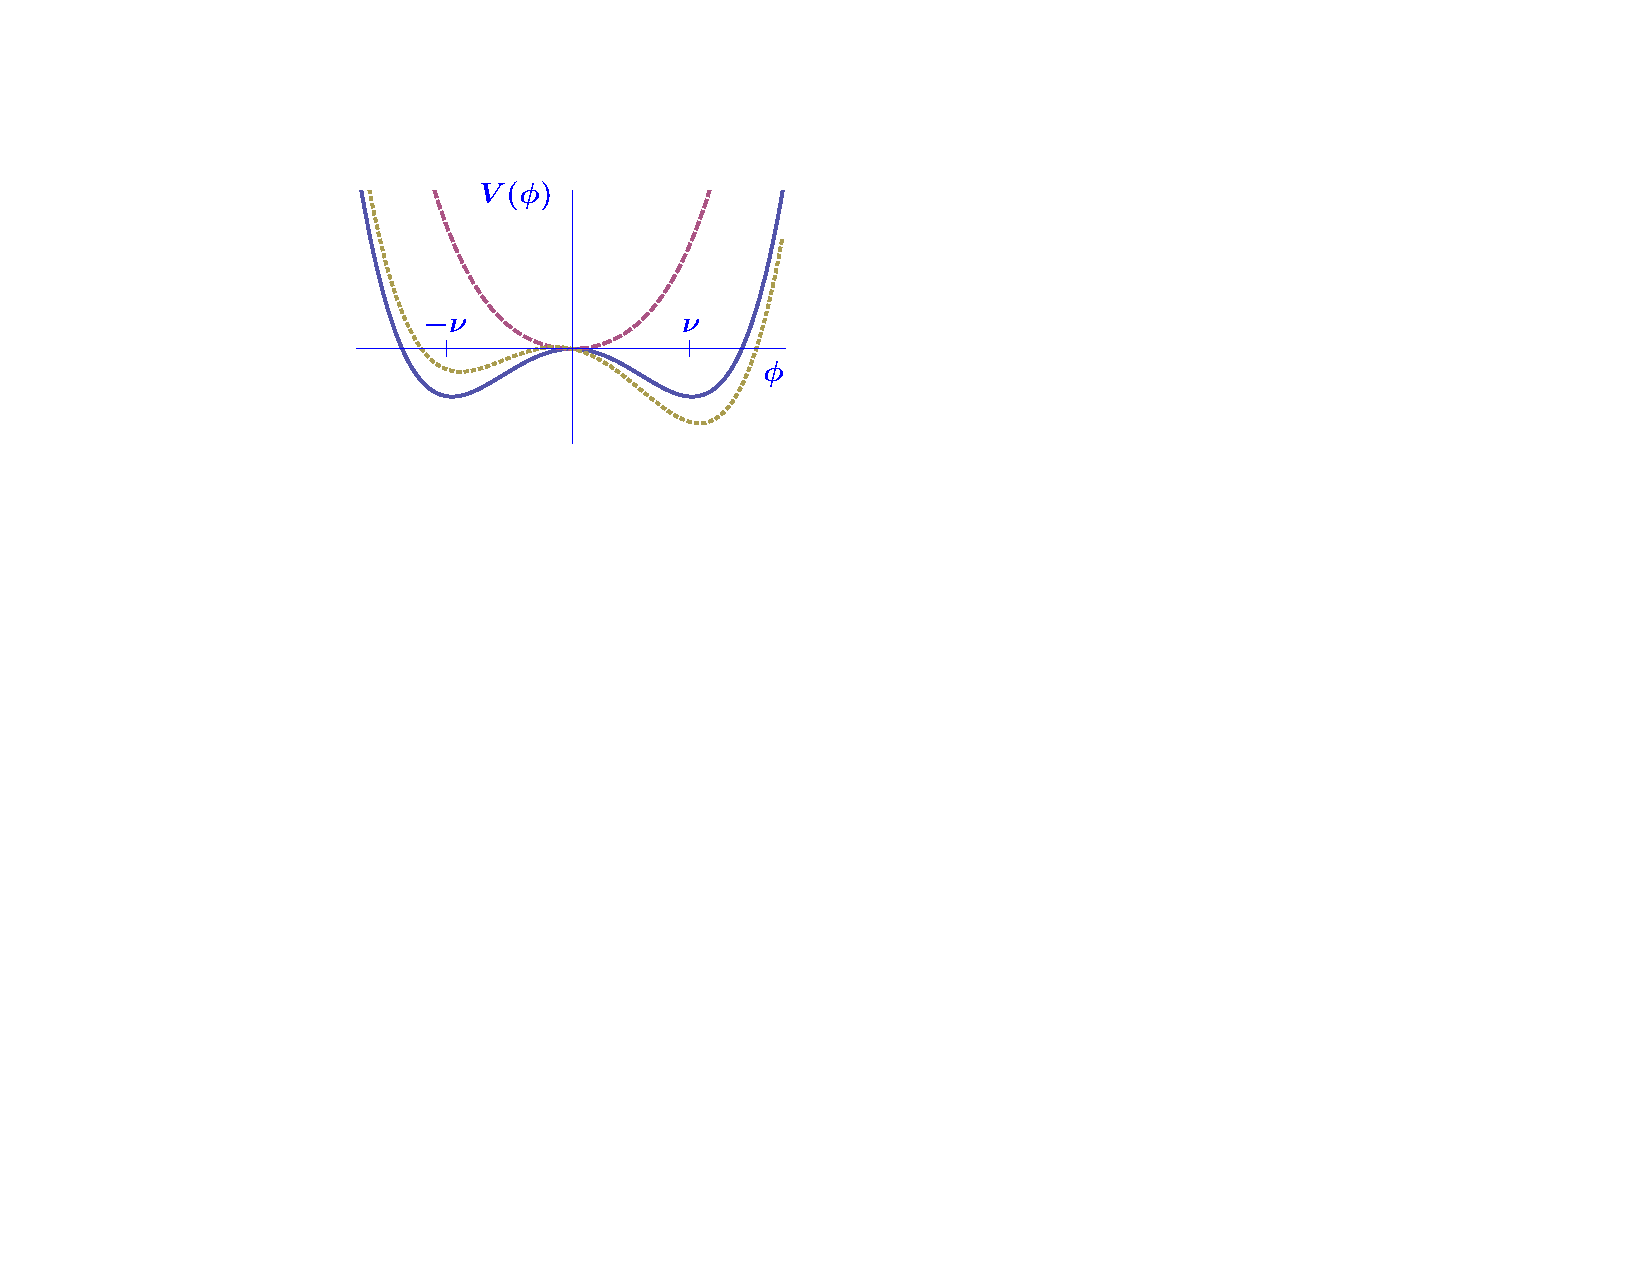
\includegraphics[width=.45\textwidth]{pics/scalar_potential}
\end{center}
\caption{Shape of the $\phi$ potential varying the values of $\mu^2$}
\label{fig:scalar_potential}
\end{figure}

This sector determines the shape of the vacuum potential and is essential to the stability of the vacuum. We require that $\lambda>0$ such that the potential is bounded from below, however $\mu^2$ can be arbitrary. If $\mu^2 >0$ we would have a minimum at $\phi=0$ and $\langle \phi \rangle =0$. If $\mu^2 < 0$ the theory becomes unstable at $\phi=0$ with alternate stable vacuum. 

As the field $\phi$ is a complex scalar field we can parameterize the field in terms
of real scalar fields $\phi_1$ and $\phi_2$:
\begin{align*}
\phi = \frac{1}{\sqrt{2}} ( \phi_1 + i \phi_2) \text{ and } \phi^\dagger = \frac{1}{\sqrt{2}} ( \phi_1 - i \phi_2)
\end{align*}
Given this parameterization, the potential becomes:
\begin{align*}
V(\phi) = \frac{1}{2}\mu^2 ( \phi_1^2 + \phi_2^2 ) + \frac{\lambda}{4} ( \phi_1^2 + \phi_2^2)^2 
\end{align*}
letting $x = \phi_1^2 + \phi_2^2$ and minimizing $\frac{\partial V}{\partial x } = 0$ we find $x_{min} = \nu$ where $\nu^2 = \mu^2/\lambda$ . 
As the vacuum is stable the theory will move to this minimum (Figure \ref{fig:scalar_potential}). Expanding
around the new vacuum $\phi_1' = \nu + \phi_1$ and $\phi_2' = \phi_2$ we obtain the new vacuum potential terms
relative to the unbroken theory:
\begin{align*}
V_{\textrm{new}} = \frac{-\mu^2}{4\lambda} - \mu^2 (\phi_1^2) + \lambda \nu \phi_1 (\phi_1^2 +\phi_2^2) + \frac{\lambda}{4}(\phi_1^2 + \phi_2^2)^2 
\end{align*}
The first of these terms is a cosmological constant and does not affect the dynamics of the theory. However,
such a constant would be relevant gravitational theories where gravity couples to energy. The Higgs Boson, $h$. the final piece of the Standard Model to be discovered is the excited mode about this new vacuum $\phi = (\nu + h(x), 0)$.
The second term is the mass term for the Higgs field. The third and fourth correspond to the cubic and quadratic self interactions. 

\begin{figure}
\begin{center}
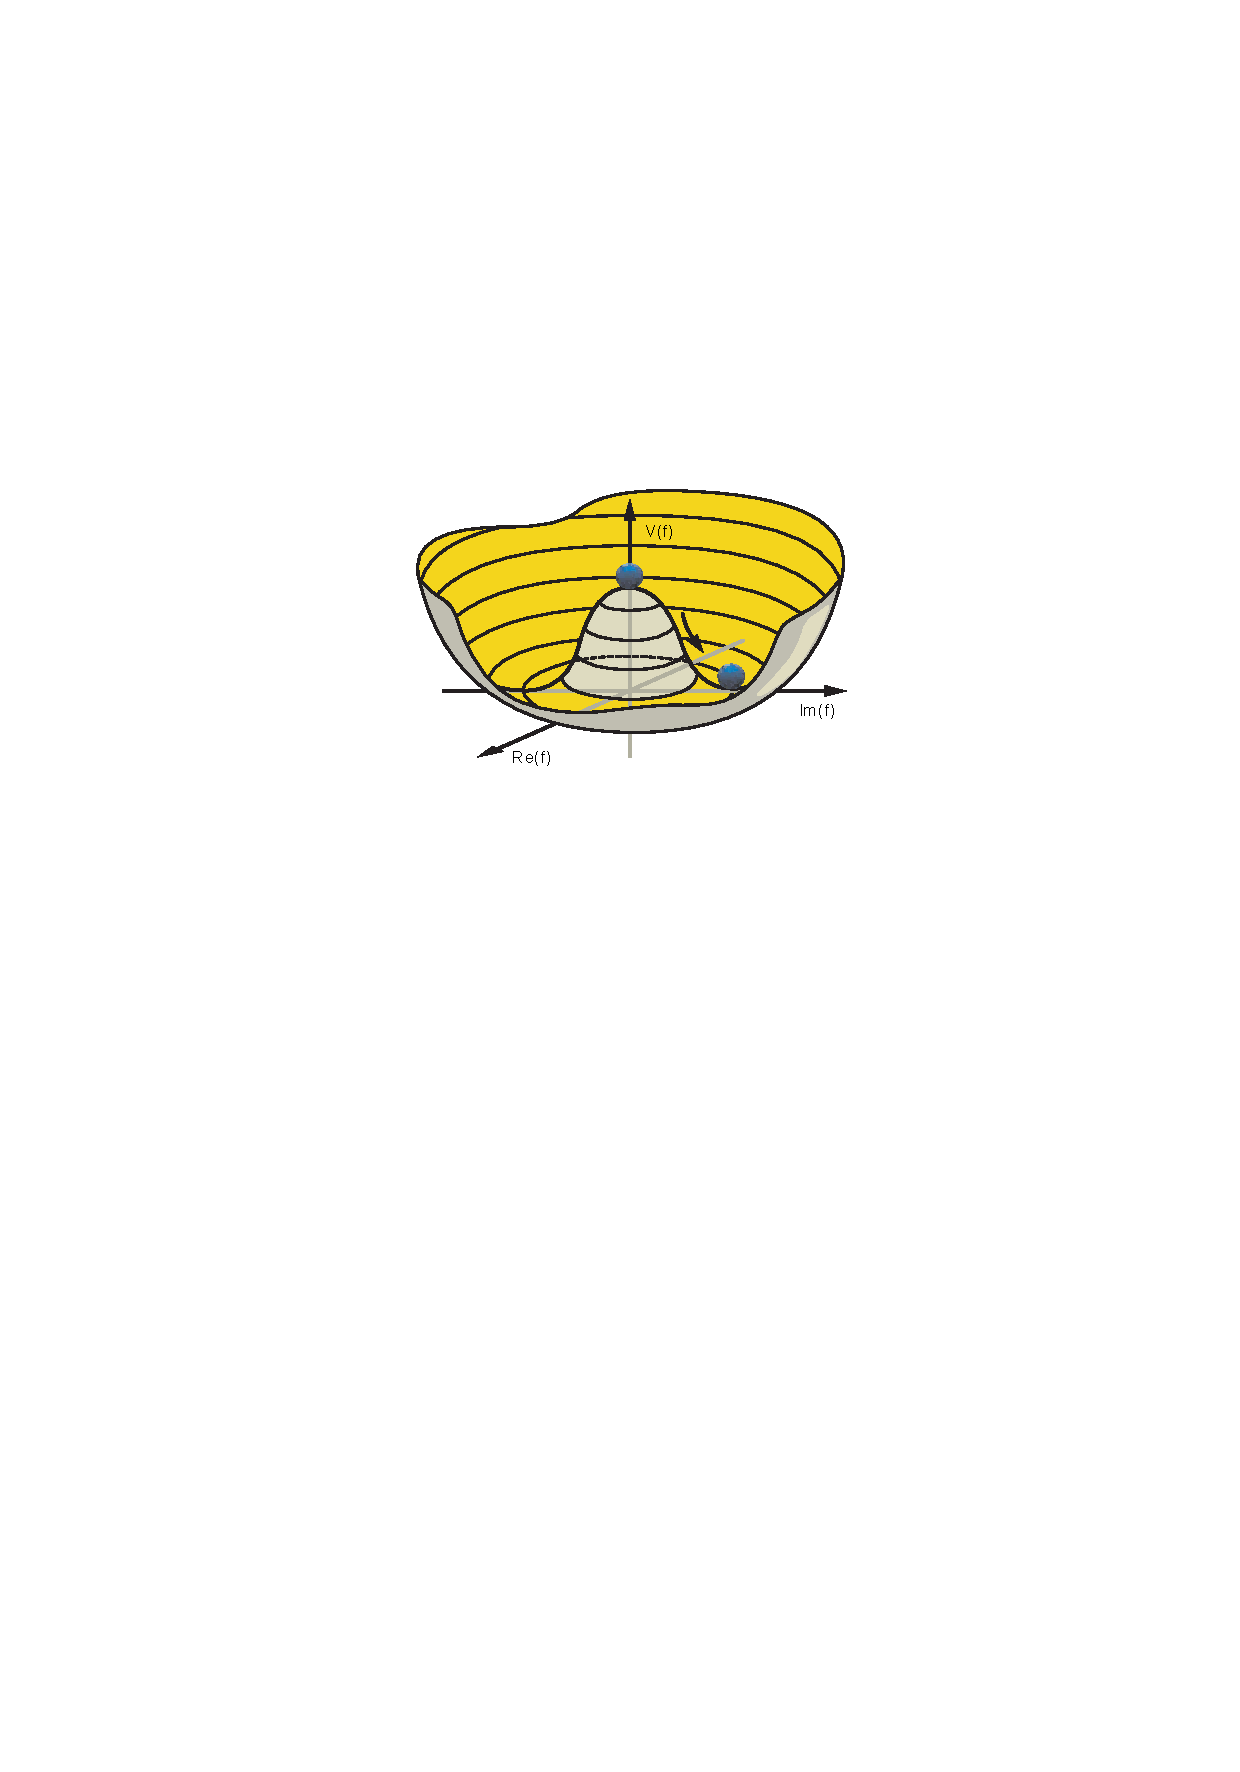
\includegraphics[width=.55\textwidth]{pics/higgs_potential}
\end{center}
\caption{The Higgs potential exhibiting spontaneously broken symmetry, where the expected vacuum expectation
value has moved from the $0$ of the theory to $\nu$ in the broken theory}
\end{figure}

If we consider the kinetic term for the field $\phi$ at the now broken vacuum $\langle \phi \rangle = (0 , \nu)$ in the gauged theory we find:
\begin{align*}
(D^\mu \phi)^\dagger (D_\mu \phi) = \frac{1}{\sqrt{2}} \left (\begin{array}{cc} 0  & \nu \end{array} \right )  \left | \partial_\mu + i g \frac{\tau}{2} \cdot W_\mu + i \frac{g'}{2} B_\mu \right|^2  \frac{1}{\sqrt{2}} \left (\begin{array}{c} 0 \\ \nu \end{array} \right ) 
\end{align*}
Considering the weak gauge term:
\begin{align*}
\tau \cdot W  = \left (\begin{array}{cc} W_{\mu,3} & W_{\mu,1} - i W_{\mu,2}  \\ W_{\mu,1}+ i W_{\mu,2} & - W_{\mu,3} \end{array} \right )
\end{align*}
adding in the diagonal $B_\mu$ terms and taking the square (ignoring the derivative terms):
\begin{align*}
(D^\mu \phi)^\dagger (D_\mu \phi) \supset \frac{\nu^2}{8} \left [g^2 (W_1^2 + W_2^2) + (g' B_\mu - g W_{\mu,3})^2 \right]
\end{align*}
Now if we perform a redefinition of the gauge fields into mass eigenstates we arrive at a clean expression:
\begin{align*}
W_{\mu}^{\pm} &= \frac{1}{\sqrt{2}}( W_{\mu,1}  \pm i W_{\mu,2} )  \\
A_{\mu} &= \frac{1}{\sqrt{g^2 + (g')^2}} (g' W_{\mu,3} + g B_\mu) = \sin \theta_W W^3_\mu + \cos \theta_W B_\mu \\
Z_{\mu} &= \frac{1}{\sqrt{g^2 + (g')^2}}( g' B_\mu - g W_{\mu,3}) = \sin \theta_W B_\mu - \cos \theta_W W_\mu^3 
\end{align*}
Here we have defined the electroweak mixing angle $\theta_W$ in terms of a right triangle with legs $g$ and $g'$. With this substitution:
\begin{align*}
(D^\mu \phi)^\dagger (D_\mu \phi) &\supset \frac{\nu^2 g^2}{4} W_{\mu}^{-} W_{\mu}^{+} + \frac{(g+g')\nu^2}{8} Z_\mu^2  + (0 \times A_\mu^2) \\ 
&= \frac{1}{2} m_{W}^2 W_\mu^- W_\mu^+ + \frac{1}{2} m_Z^2 Z_\mu^2  + (0 \times A_\mu^2)
\end{align*}
EWSB has generated the mass terms for the gauge bosons! 
$m_{W^{\pm}} = \frac{\nu g}{\sqrt{2}} = 80.385$~[GeV],
$m_Z = \frac{\nu}{2}\sqrt{g+g'} = \frac{m_W}{\cos \theta_W} = 91.1876$~[GeV]  and the massless photon $A_\mu$. 

\subsection{Maxwell's Laws} 

After EWSB we can perform a sanity check by deducing the well studied equations governing
 electrodynamics from the QFT description. Keeping only the terms that contain the field $A_\mu$:
\begin{align*}
\mathcal{L}_{EM} = -\frac{1}{4} F_{\mu\nu} F^{\mu\nu}  - ie \bar{\psi} \gamma^\mu A_\mu \psi \text{ for } F_{\mu\nu} = \partial_\mu A_\nu - \partial_\nu A_\mu 
\end{align*}
where by definition $F_{\mu\nu} = \partial_\mu A_\nu - \partial_\nu A_\mu$. Applying the left side of Euler-Lagrange we find:
\begin{align*}
\partial_\mu \left (\frac{\partial \mathcal L}{\partial(\partial_\mu A_\nu)} \right) &=  
-\frac{1}{2}\partial_\mu \left [ \left (\frac{\partial}{\partial(\partial_\mu A_\nu)} F_{\mu\nu} \right) F^{\mu\nu} \right ] 
= -  \partial_\mu F^{\mu\nu}
\end{align*}
The other term is simply $\frac{\partial \mathcal L}{\partial A_\mu} = -ie \bar \psi \gamma^\mu  \psi = - J^\mu = -(\rho, \vec J)$. Where $\rho$ is charge
density and $\vec J$ is current. This yields our first equation:
\begin{equation}
\partial_\nu F^{\nu\mu} = J^\mu
\end{equation}
recognizing the field tress tensor is antisymmetric we can apply a partial derivative and contract with the indices of the 4 dimensions anti-symmetric symbol
to obtain:
\begin{equation}
\epsilon_{\theta\rho\mu\nu} \partial_{\rho} F_{\mu\nu} = 0 
\end{equation}
Using these two laws we first see that the electric and magnetic field, $E$ and $B$, can be
defined in terms of the field stress tensor
\begin{align*}
F_{0i} = \partial_0 A_i - \partial_i A_0 = -\frac{\partial A}{\partial t} - \nabla \Phi = E
\end{align*}
As for the magnetic field $B_i$:
\begin{align*}
\epsilon_{ijk}B^k &= \epsilon_{ijk} \epsilon_{klm} \partial_l A_m = \epsilon_{kij} \epsilon_{klm} \partial_l A_m = (\delta_{il} \delta_{jm} - \delta_{im}\delta_{jl}) \partial_l A_m = \partial_i A_j - \partial_j A_i = F_{ij}
\end{align*}
From the first current law we immediately obtain two of Maxwell's laws:
\begin{align*}
\partial_i F^{0i} = J^0 \implies \nabla \cdot E = \rho
\end{align*}
and for the second we separate the sum between space and time-like components:
\begin{align*}
\partial_i F^{ji} + \partial_0 F^{j0} = J^j\\
\epsilon_{jik} \partial_i B_k - \partial_0 E^j = J^j\\
\nabla \times B - \frac{\partial E}{\partial t} = \vec J
\end{align*}
The remaining two laws come from manipulations of the antisymmetry of the field stress tensor:
\begin{align*}
0 = \epsilon_{0ijk} \partial_i F^{jk} =
\epsilon_{0ijk} \partial_i \epsilon_{0jkl} B_l =
\epsilon_{jk0i}  \epsilon_{jkl0} \partial_i B_l  =
-\delta_{il} \partial_i B_l  \\
\implies \nabla \cdot B = 0
\end{align*}
The time component of the field stress tensor in the last equation in terms of $E$ and $B$ yields
\begin{align*}
\epsilon_{\mu\nu0\sigma} \partial_\nu F^{0\sigma} + \epsilon_{\mu\nu i\sigma} \partial_\nu F^{i\sigma}&= 0 \text { for } i=1,2,3\\
\epsilon_{0\sigma\mu\nu} \partial_\nu E^{\sigma} + \epsilon_{\mu\nu i\sigma}  \epsilon_{0i\sigma k} \partial_\nu B_k&= 0 \text{ where } k\neq 0\\
\end{align*}
The first term is $\nabla \times \vec E$. Separately expanding the second term by permuting the $\epsilon$ indices
\begin{align*}
&\epsilon_{i\sigma \mu\nu}  \epsilon_{i\sigma k 0}  \partial_\nu B_k \text{ where } k\neq 0\\
=&(\delta_{uk} \delta_{\nu 0} - \delta_{\mu 0} \delta_{\nu k} )  \partial_\nu B_k\\
=& \partial_0 B_\nu - \partial_k B_k&\\
=&\frac{\partial \vec B}{\partial t} - \nabla \cdot \vec B\\
=&\frac{\partial \vec B}{\partial t}&
\end{align*}
The last line used $\nabla \cdot \vec B = 0$. Combining the two terms:
\begin{align*}
\nabla \times \vec E + \frac{\partial \vec B}{\partial t}&= 0
\end{align*}
We should not forget that the assumptions that led us to these equations. Firstly, the  existence of the field stress tensor. We obtained this by writing
 the most general Lorentz invariant and gauge invariant Lagrangian possible. Additionally, we made geometric arguments about the continuity
  in the derivative under the local $U(1)$ gauge symmetry in the Lagrangian to obtain the interaction term between 
the gauge boson and the electron $\psi$ . Everything 
we understand from the study of electromagnetism naturally 
arises from the Standard Model Lagrangian. This even includes 
the curiosity of electromagnetism that when the theory is written in terms of vector and scalar potential the equations remain
 unchanged under a gauge transformation. However, in a gauge theory 
this is the fundamental principle rather than a consequence of the form of Maxwell's equations. I feel compelled to note that this is amazing. 

\subsection{Feynman Diagrams}
\begin{figure}
\begin{center}
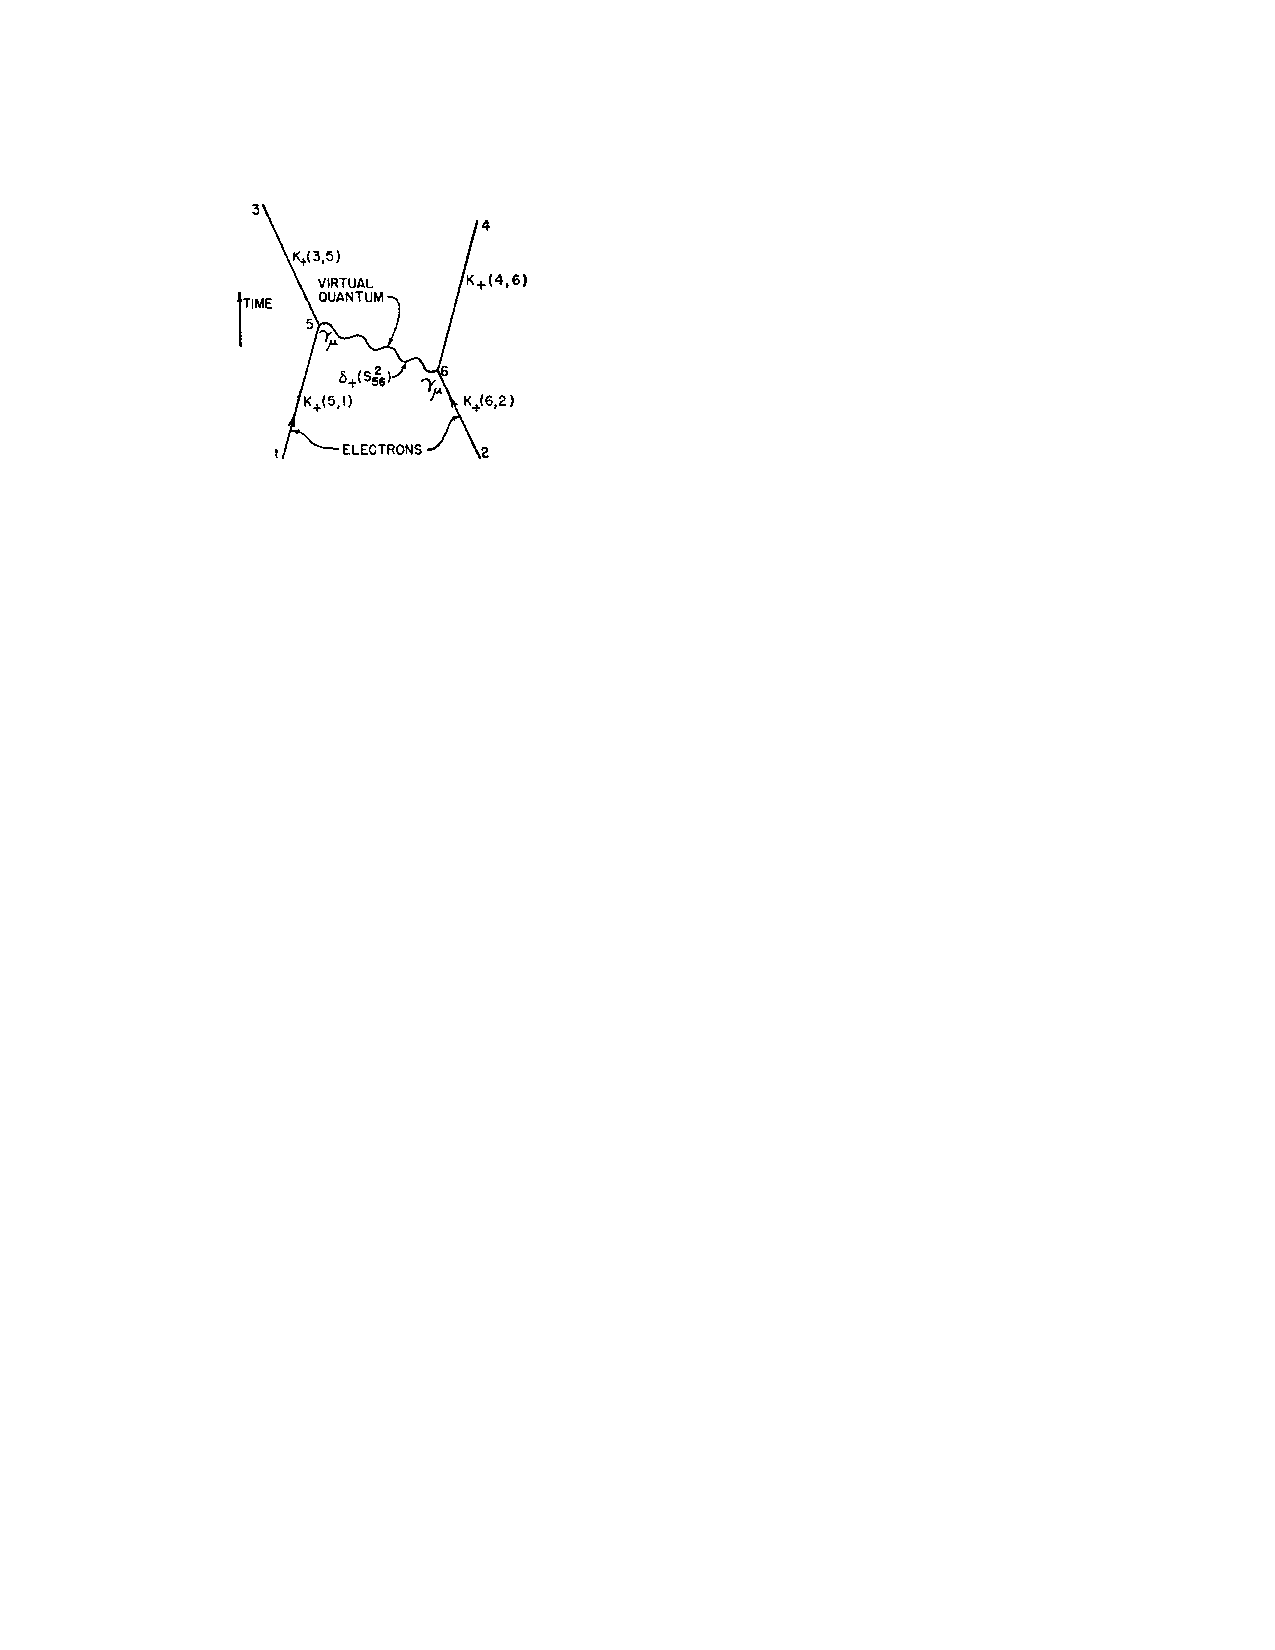
\includegraphics[width=.450\textwidth]{pics/first_diagram}
\end{center}
\caption{The Feynman diagram for describing t-channel scattering of two electrons through
the exchange of a virtual photon. This particular figure
 was the example used in Feynman's original paper describing the pictorial representation of calculating matrix elements.}
\label{fig:first_diagram}
\end{figure}
Historically, the outcome of a scattering event in a quantum field theory was
 tedious to calculate. One of Feynman's greatest contributions to the field of
 particle physics was an organizational tool to group and quickly calculate terms 
in the perturbative expansion of the action \cite{feynman}. The diagrams, Feynman diagrams (Figure \ref{fig:first_diagram}), 
take the form of a directed graph of lines and vertices providing a  representation
the components needed in a scattering calculation calculation. This treatment is
intuitive to work with and incredibly information dense minimal effort to construct. 
In this section we will derive principal aspects of how scattering events can be represented leaving the subtleties to the references \cite{peskin,Srednicki}.

We write down a simple scalar quantum field theory with a single scalar field $\phi$ and a $\phi^3$ interaction term:
\begin{align*}
\mathcal{L} = \mathcal{L}_0 + \mathcal{L}_{int} = \frac{1}{2}(\partial_\mu \phi) (\partial^\mu \phi) + m^2 \phi^2 - \frac{\kappa}{3!} \phi^3 
\end{align*}
In the Schr\"odinger picture of quantum mechanics the states $|\psi \rangle$  evolve in time 
according to the Hamiltonian $H_S=H_0+H_{int}.$  The component $H_0$ is the free particle component and $H_{int} = - \mathcal{L}_{int}$ is the interacting component. The quantum state obeys the Schr\"odinger equation:
\begin{align*}
i\frac{d}{dt} |\psi \rangle = H_S | \psi \rangle
\end{align*}
This gives we obtain the solution $|\psi(t,x) \rangle =  U(t,0)| \psi(0,x) \rangle$ where we define
the time evolution operator $U(t,t_0) = \exp{(-iH_S (t-t_0))}$.  The observables are constant in time
and the expected value of some operator (in our case the quantum field $\phi$) on a state
at time $t$ can be written:
\begin{align*}
\langle \phi(t,x) \rangle = \langle x,t_0 | e^{iH_S(t-t_0)} \phi(x) e^{-iH_S(t-t_0)} | x,t_0 \rangle 
\end{align*}
In this interpretation of quantum mechanics, we instead absorb the time dependence into the operator, leaving the states constant.
\begin{align*}
 \phi(t,x) =   e^{iH_St} \phi(x)  e^{-iH_St}
\end{align*}
Let us define a new interacting field $\phi_I = e^{iH_0t} \phi  e^{-iH_0t}$ which evolves
 with the free Hamiltonian. In the Heisenberg picture, the field can be written in terms of $\phi_I$ as:
\begin{align*}
 \phi(t,x) &=   e^{iH_St}e^{-iH_0t} \phi_I(x) e^{iH_0t} e^{-iH_St} = U^\dagger(t) \phi_I U(t)
\end{align*}
We have defined a unitary operator $U(t)=e^{iH_0t}e^{-iH_St}$. If we apply a time derivative to $U(t)$ we find:
\begin{align*}
i\partial_t U(t) &= -e^{iH_0t}H_0 e^{-iH_St} + e^{iH_0t} H_S e^{-iH_St}\\
&= e^{iH_0t}H_{int}e^{-iH_St}\\
&= e^{iH_0t}H_{int}e^{-iH_0t}e^{iH_0t}e^{-iH_St}\\
&= H_I U(t) = \left (\frac{\kappa}{3!}\phi_I^3 \right) U(t)
\end{align*}
We have shown the time evolution operator obeys the Schr\"odinger equation under a Hamiltonian $H_{I}$, corresponding to
 $H_{int}$ in the Heisenberg picture. Solving this equation, we obtain a time evolution
operator $U(t) = T\exp (-\int dt iH_I)$. The operator $T$ denotes time ordering of the time integrals for each term
in the series expansion of the exponential which will not necessarily commute. 
 Since each $H_I(t)$ will be integrated against its own dummy time variable, the time ordering operator will place $H_I(t)$ terms farther to the left,
 if they occur later in time. The reason for this time ordering requires detail that can be found in the references \cite{peskin,Srednicki}.

We have succeeded in writing the time evolution operator in terms of the field $\phi_I$. which evolves according to the free Hamiltonian 
where we we already have a solution expressed in terms of creation and annihilation operators:
\begin{align*}
\phi_I(\vec x, t) = \int \frac{d^43}{(2\pi)^3\sqrt{2E}} \left [  a_p e^{ipx} + a_p^\dagger e^{-ipx} \right ]
\end{align*}
Now when we would compute the matrix element of $\phi\phi$ scattering, we expand the time evolution operator:
\begin{align*}
U(t,0) &= 1 - i \int_0^t H_I(t)  - \frac{1}{2} \int_0^t dt \int_0^{t'} dt' T\{ H_I(t) H_I(t')\} \ldots \\
&= 1 - i \frac{\kappa}{3!}\int d^4x \phi^3(x)  - \frac{1}{2} \frac{\kappa^2}{3!3!} \int d^4x \int d^4x' T \{ \phi^3(x) \phi^3(x') \}  \ldots 
\end{align*}
For a matrix element $\mathcal{M}$ if $\kappa<1$ the theory is perturbative and the first non-zero term
will dominate. For $2\rightarrow 2$ scattering this 
term will be at order $\kappa^2$ and is computed by expanding the fields in terms
of the creation and annihilation operators. Since $a|0\rangle = \langle 0 | a^\dagger = 0$, the only terms which will contribute will be the terms with equal numbers of creation and annihilation operators coming from the $\phi^3(x)\phi^3(x')$ term. 

Rather than expanding all of these fields, we use a result known as Wick's Theorem
to convert the time ordered product into a series of pair-wise contractions between the individual fields. 
A contraction is defined for a field $\phi$ in terms of its positive and negative 
frequency components $\phi_I = \phi^+_I +\phi^-_I$ where the $+$ field contains the annihilation operator, and $-$ the creation operator.
%\contraction{}{}{$\phi$}{$(x)$}{$\phi$}(y)
\begin{align*}
\begC1{\phi}\conC{(x)}\endC1{\phi}(y)  = [\phi^+(x),\phi^-(y)] \text{ if } x^0 > y^0 \text{ else } [\phi^+(y),\phi^-(x)] 
\end{align*}
Given this definition, we state Wick's theorem as:
\begin{align*}
T[\phi_1(x_1) \ldots \phi_N(x_N) ] = N \left [ \phi_1(x_1) \ldots \phi_N(x_N) + \text{ all possible contractions }      \right ]
\end{align*}
Where $N$ is the normal ordering operator which operates on a sequence of creation and annihilation operators by moving
all creation operators to the left and annihilation operators to the right. By normally ordering a term
in the expansion, we can eliminate all un-contracted terms as they will annihilate the vacuum. In lieu of a proof of Wick's theorem
(which can be shown by induction) we can consider the process of taking the original term and moving creation
 operators to the left using commutation relations. Each time an operator is moved closer to its
 normal ordered configuration, we pick up a commutator between two elements with enters the expansion
as a contraction. In fact, all possible contractions will be produced. When we are left with only normal ordered terms, if a term is not fully contracted the term will annihilate the vacuum state. Lets enumerate the contractions on a $\phi^4$ term:
\begin{align*}
&\left(\begC1{\phi}\conC{_1}\endC1{\phi_2}\phi_3 \phi_4 +  \phi_1 \phi_2 \begC1{\phi}\conC{_3}\endC1{\phi_4} +
 \begC1{\phi_1}\conC{\phi_2\phi_3}\endC1{\phi_4} +  \begC1{\phi_1}\conC{\phi_2} \endC1{\phi_3}\phi_4 +
\phi_1\begC1{\phi_2} \endC1{\phi_3}\phi_4 + \phi_1\phi_2 \begC1{\phi_3}\endC1{\phi_4}  \right)  + \\
&\left (\begC1{\phi}\conC{_1}\endC1{\phi_2}\begC1{\phi}\conC{_3}\endC1{\phi_4} + \begC1{\phi_1}\begC2{\phi_2}\endC1{\phi_3}\endC2{\phi_4} + \begC1{\phi_1}\begC2{\phi_2}\endC2{\phi_3}\endC1{\phi_4} \right)
\end{align*}
We have not yet considered the initial and final states. The external observable states of the diagram when evaluated on a fully contracted term correspond to an unscattered state. However, we are only interested in cases where
the states have scattered. The only contributing terms are those where the number of inner + outer states is equal to the number of 
uncontracted fields in the inner term. A scalar field operating on the outer states give just a factor of 1 
 (equivalently a phase in momentum space) times the vacuum $\Omega$. We can think of these
terms as contractions between inner and outer states:
\begin{align*}
\langle\begC1{p_f}\conC{|}\endC1{\phi} = \langle \Omega |   \text{  and  } \begC1{\phi}\conC{|}\endC1{p_i}\rangle =  | \Omega \rangle
\end{align*}
To summarize, for a given term in the Lagrangian, if we restrict ourselves to scattered states, we need to have
a full contracted term that includes the outer states. If we return to our $\phi^3$ theory and attempt to scatter
$\phi\phi\rightarrow\phi\phi$ we would need 4 $\phi$ fields to contract with the outer states. So at lowest order, this 
means we need a $\phi^3(x)\phi^3(y)$ term where two of the internal fields are contracted between $x$ and $y$. If 
we had no contraction between the $x$ and $y$ terms, this would yield one term which would only be connected to 
a single outer state. If this is the case, the in going states $p_1,p_2$ would yield final states with momentum 
$p_3$ and $p_1+p_2$,  momentum conservation  means $p_3=0$, so we do not include it in the calculation. It can be shown 
that all disconnected diagrams will not contribute to $\mathcal{M}$. An example contributing term would look like:
\begin{align*}
\frac{(-i\kappa)^2}{2*3!*3!}\langle \begC1{p_1}\begC2{ p_2}\conC{|}\endC1{\phi(x)} \endC2{\phi(x)} \begC1{\phi(x)}\endC1{\phi(y)} \begC1{\phi(y)}\begC2{\phi(y)}\conC{|}\endC2{p_3}\endC1{p_4} \rangle
\end{align*}
For the first $\phi^3(x)$ term we have 3! choices of pairing two fields with a single outer state (and same
for the second $\phi^3(y)$). There is an additional factor two for interchanging which outer state contracts 
with $\phi^3(y)$ or $\phi^3(x)$. Knowing
where we were headed, we have already included the combinatorial factor with the coupling constant.
With this normalization of the coupling, each non-zero term will include a propagator and 
a factor $(-i\kappa)^2$. Moving to momentum space,
 the inner contractions (propagators) correspond to the Greens function
 of the free Klein-Gordon equation:
 $[\phi(x),\phi(y)] = i / (p^2 - m^2)$. There are three unique terms. 
The terms correspond to the three possible ways the outer momentum states can be contracted with the two terms.
\begin{align*}
(-i\kappa)^2\left( \frac{i}{(p_1+p_2)-m^2} + \frac{i}{(p_1-p_3)-m^2} + \frac{i}{(p_1-p_4)-m^2} \right)
\end{align*}

\begin{figure}
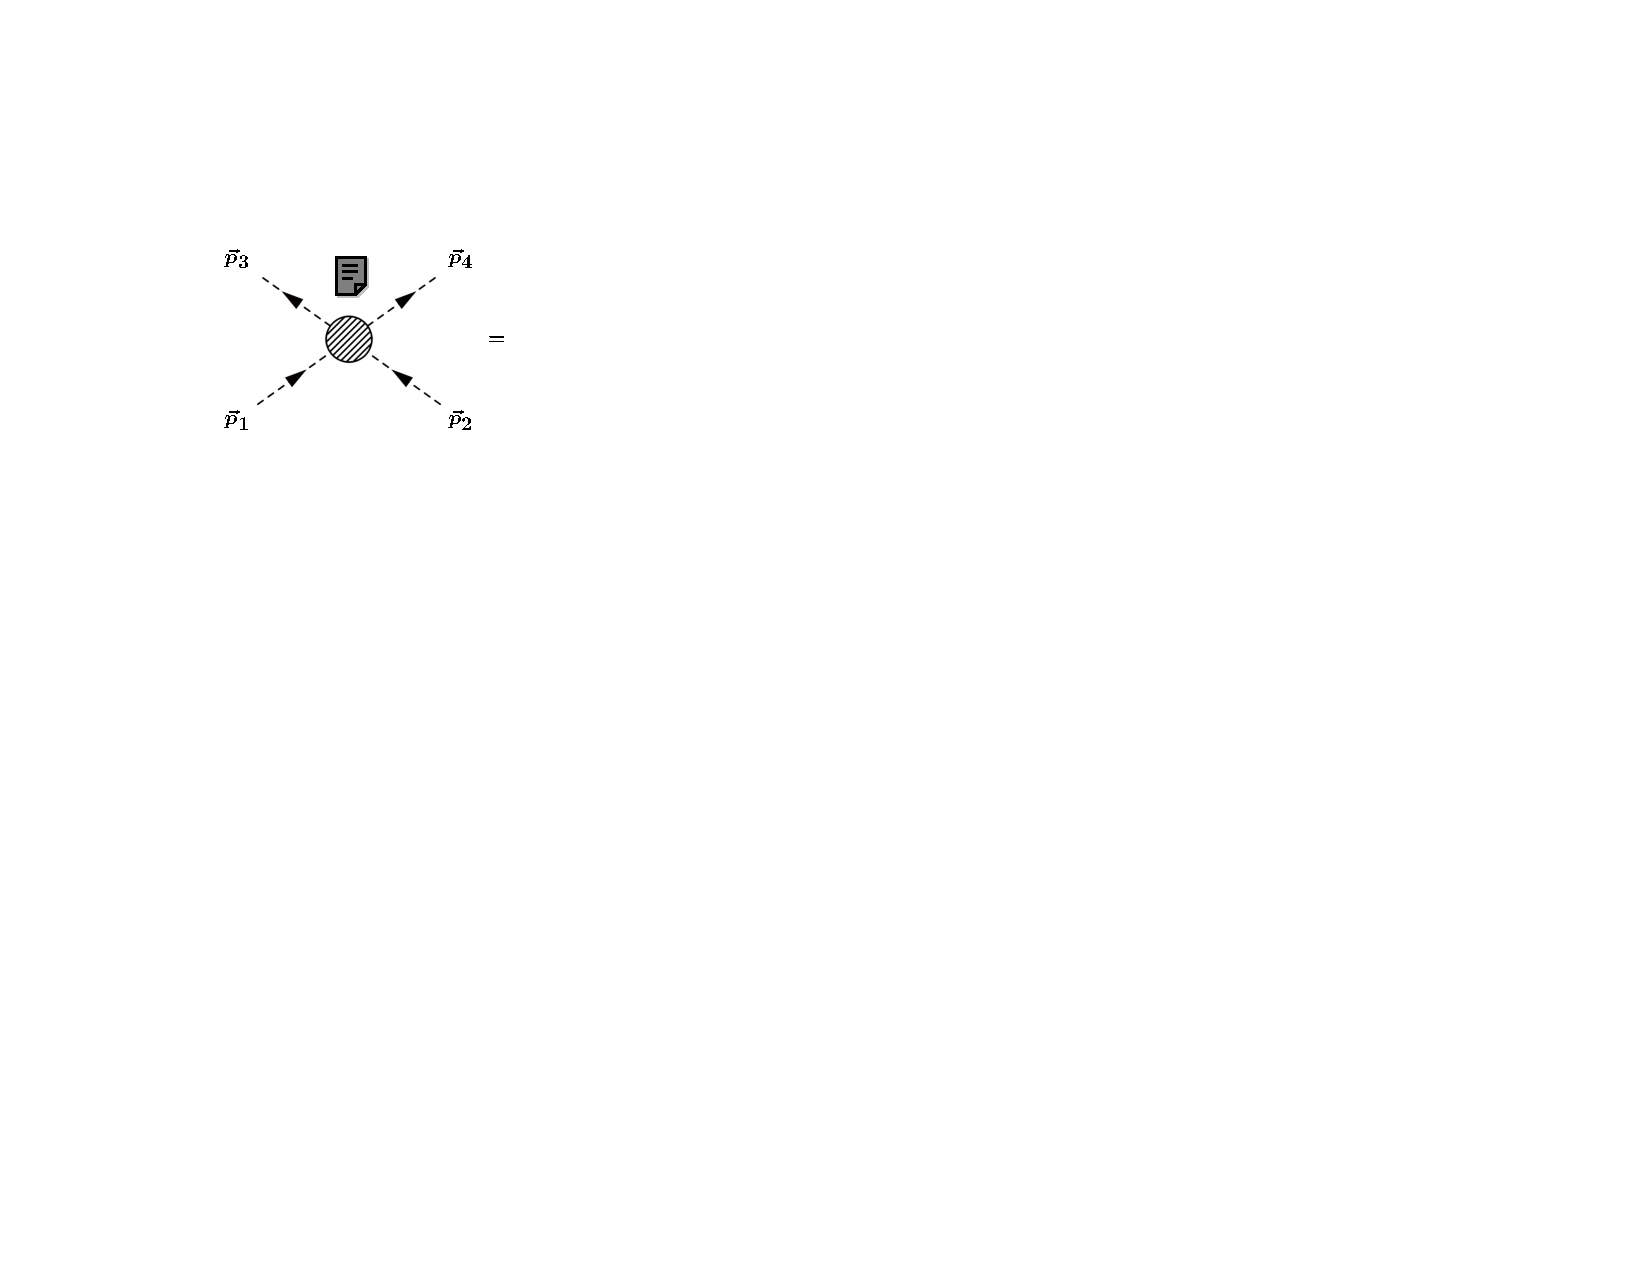
\includegraphics[width=.31\textwidth]{pics/interaction}\\
\begin{center}
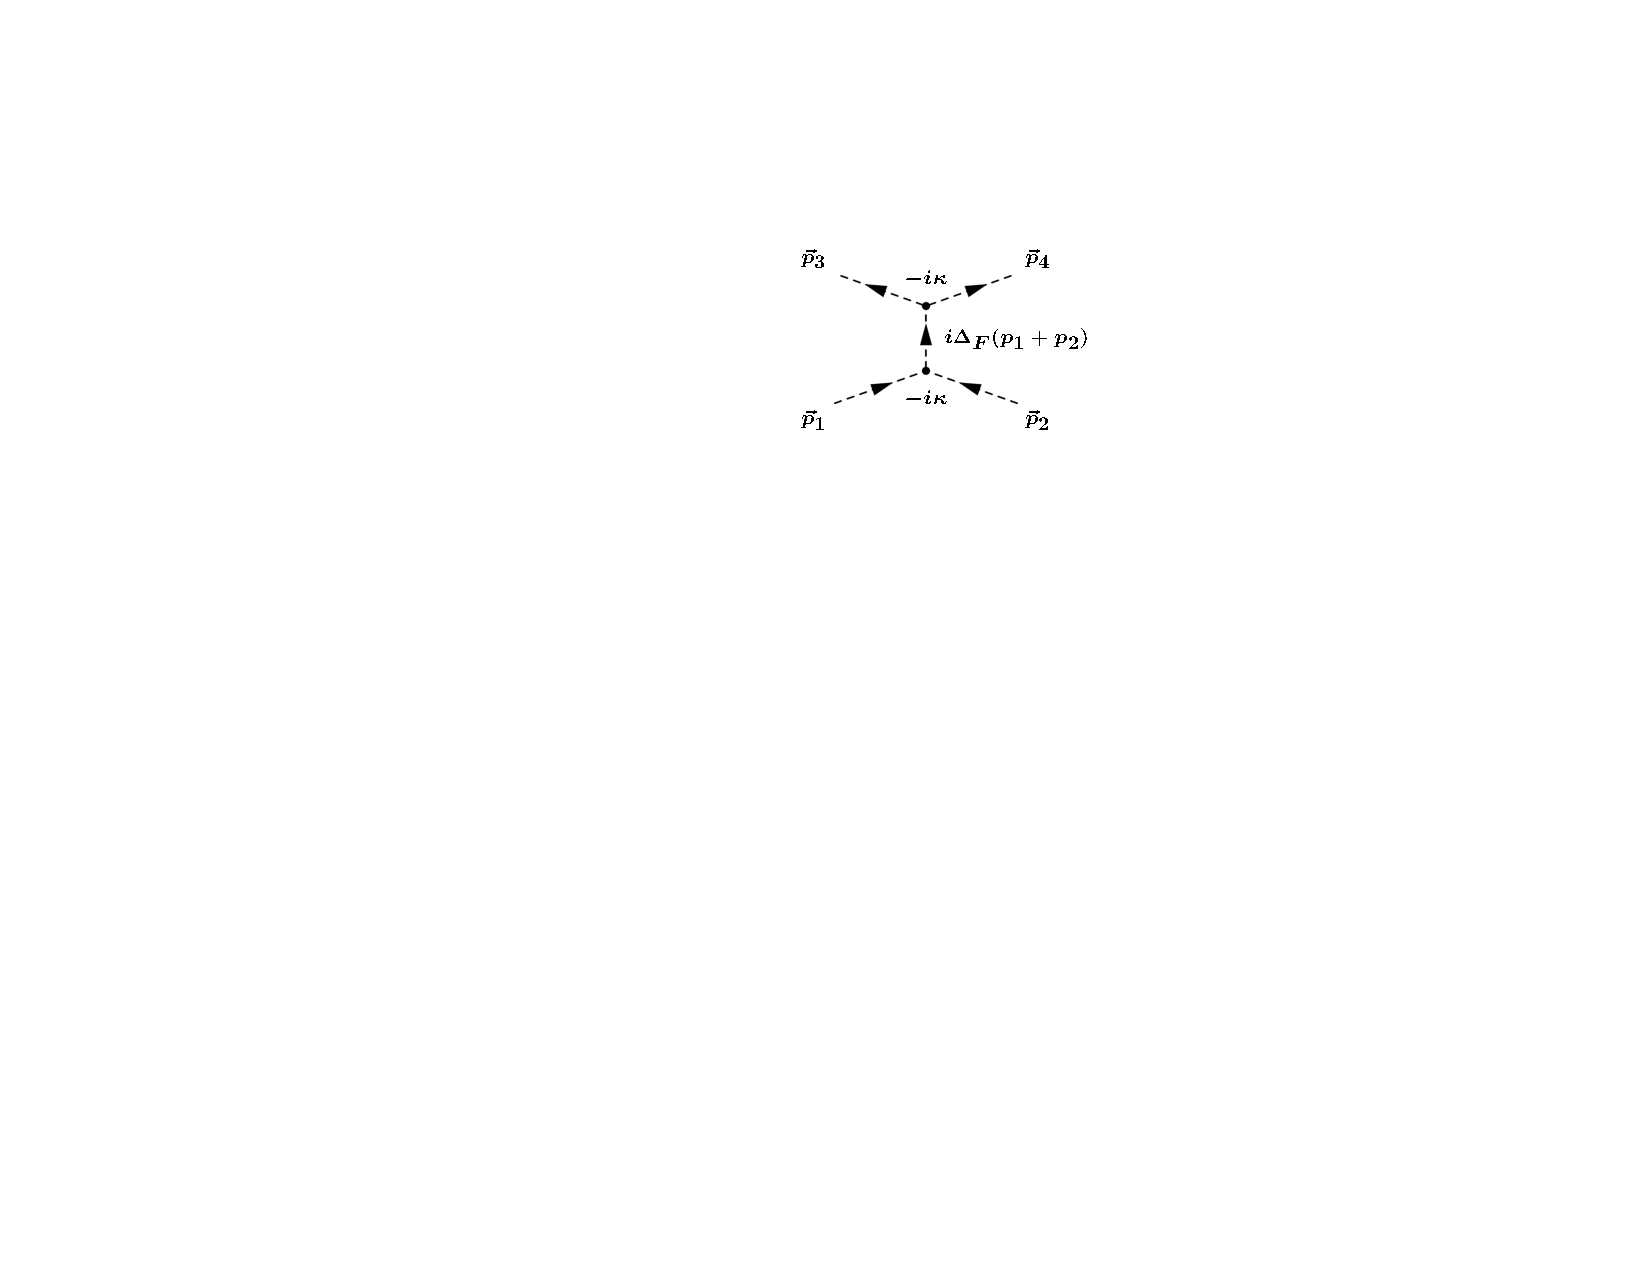
\includegraphics[width=.31\textwidth]{pics/s_diagram}
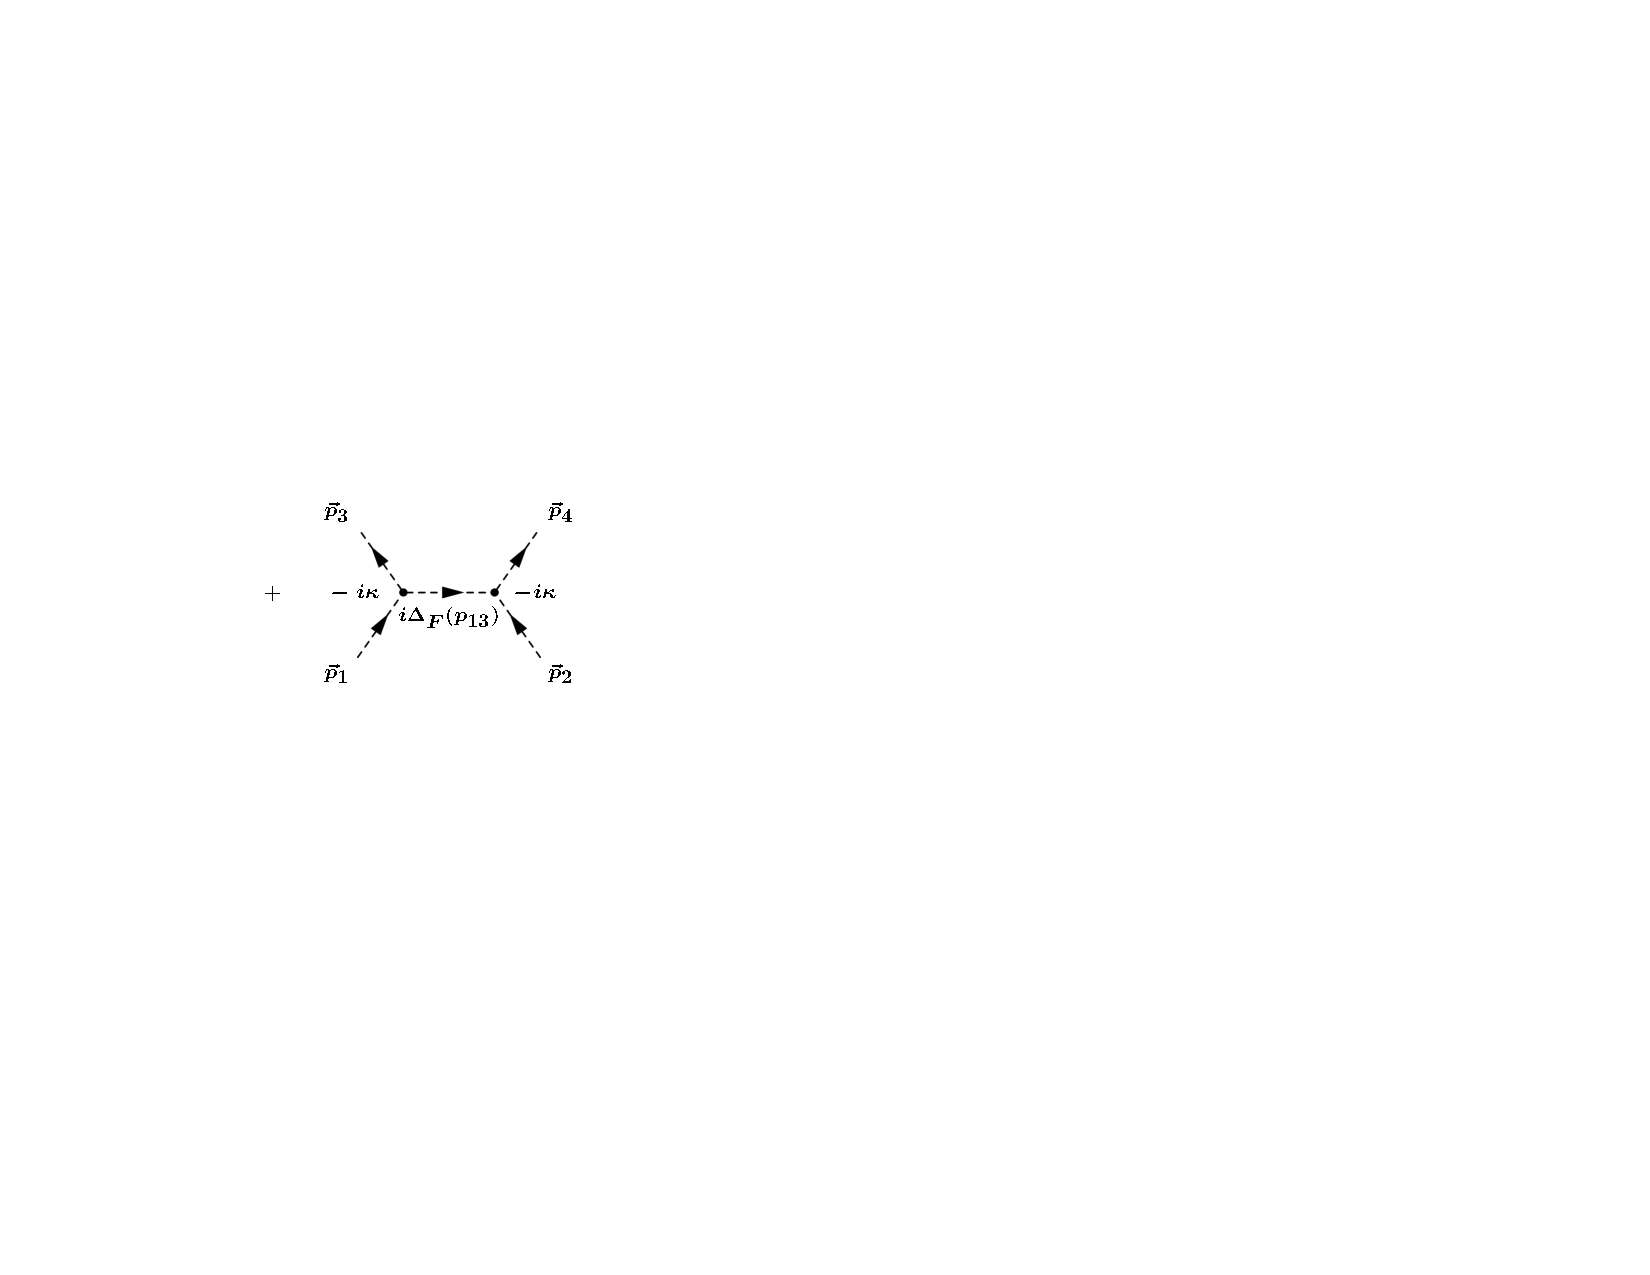
\includegraphics[width=.31\textwidth]{pics/t_diagram}
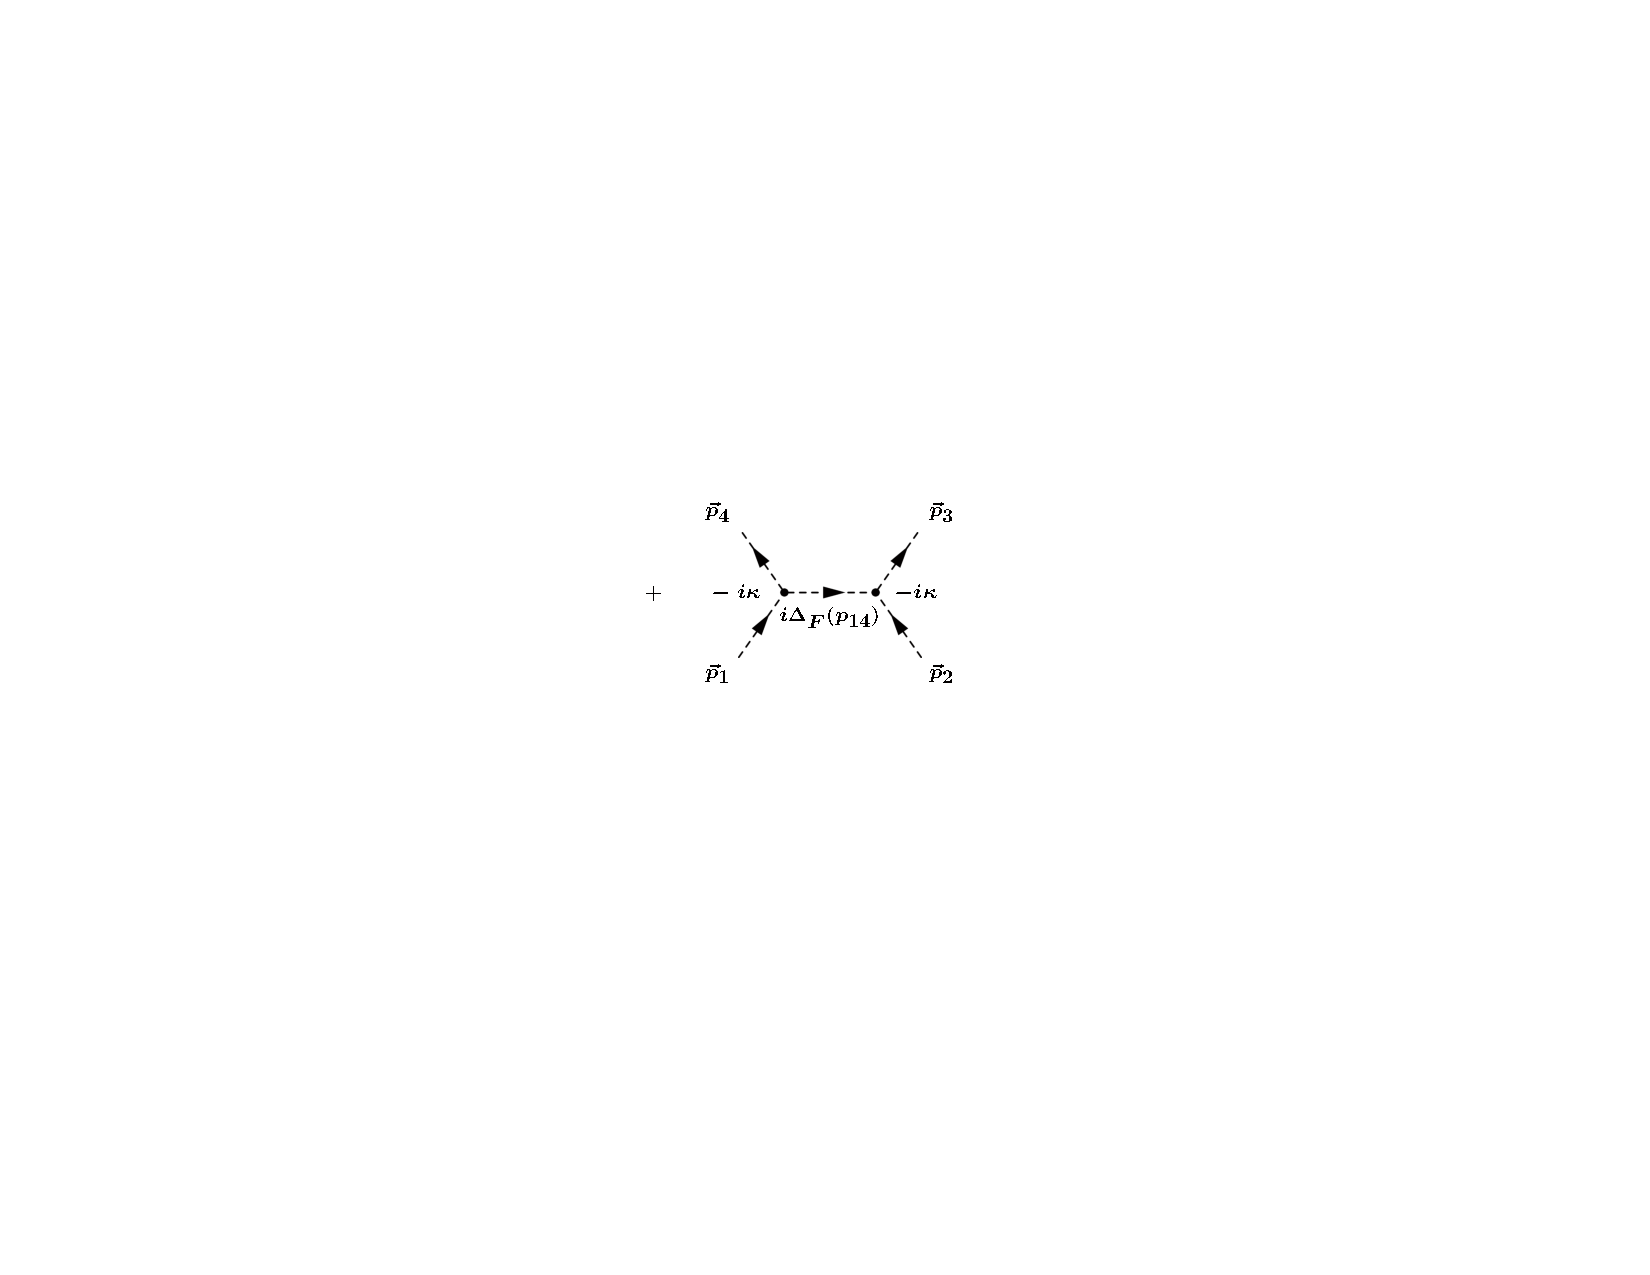
\includegraphics[width=.31\textwidth]{pics/u_diagram}
\end{center}
\caption{The 3 diagrams corresponding to $\phi\phi\rightarrow \phi\phi$ scattering at tree level (leading order). Time
is directed vertically.}
\label{fig:stu_diagrams}
\end{figure}

This is where the wonderful simplicity of Feynman diagrams enters the picture. 
The structure of contractions can be represented
visually by vertices connected by lines (Figure \ref{fig:stu_diagrams}). Our $\phi^3$ term 
in the Lagrangian represents a vertex with 3 legs corresponding to the three $\phi$ fields. 
The vertex itself introduces the coupling constant (when normalized properly) and the legs are then connected to an
outer state or another vertex. The unconnected legs are
the contractions with outer states. These legs are physical and
 are referred to as external lines. 
The legs connected between vertices are virtual and referred to as internal lines. 

Since these products and differences of momentum are common in particle physics we use
the conventional Mandelstam variables, which add a reduction in notation. The variables can also be written in terms
of the 2$\rightarrow$2 scattering angle and the center of mass energy of the collision. 
\begin{align*}
s&=(p_1+p_2)^2 = 4(p^2+m^2) = E_{cm}^2 \\
t&=(p_1-p_3)^2 = -2p^2(1-\cos\theta)\\
u&=(p_1-p_4)^2 = -2p^2(1+\cos\theta) 
\end{align*}
Here the scattering angle $\theta$ is defined as $\hat p_i \cdot \hat p_f$ in the center 
of mass frame. Summing the diagrams appropriately named the $s,t,$ 
and $u$-channel diagrams, we calculate the un-squared amplitude. 
\begin{align*}
\mathcal{M} = (-i\kappa)^2\left( \frac{i}{s-m^2} + \frac{i}{t-m^2} + \frac{i}{u-m^2} \right)
\end{align*}
The rate of this process is proportional to $|\mathcal{M}|^2$. The exact way this corresponds to what we observe in 
the detector is left to the following section.

In practice, one can avoid needing to compute the combinatorics of contractions by simply knowing 
the terms contained in the theory, and the Feynman ``rules'' for particular fields 
(spin-0, spin-1, spin-$\frac{1}{2}$). For a spin-0 field the Feynman rules are:
\begin{itemize}
\item Internal lines: $\Delta(p) = \frac{i}{p^2 - m^2+i\epsilon}$. The epsilon enforces a pole prescription for the integral the corresponds to causal propagation of the
virtual quantum. 
\item Vertices: $-i\kappa$
\item Symmetry Factors: Account for possible symmetries in the diagram that would over count the multiplicities of diagrams. These factors are rare except higher order diagrams. Calculations by hand are rarely more than a factor 2. 
\item Momentum Conservation: Require that four momentum is conserved at each vertex. This condition was enforced by the phases in the quantum fields, but is put in by hand in the diagrams.
\item Integrate over any undetermined momentum. 
\end{itemize}
%% To calculate a given scattering amplitude, one simply constructs all of the applicable diagrams between
%% the incoming particles (ex. proton-proton) and the outgoing final state  (ex. $q\bar{q}$). Lines represented particles with a given momentum and vertices represented
%% interaction terms in the lagrangian where four-momentum conservation was enforced. Internal 
%% lines of the diagram, that is, neither initial nor final state particles, were virtual 
%% particles were space-like. 
Given an initial and final state, one uses the vertices as building blocks to construct all 
connected diagrams at the chosen order in the coupling. The rules then dictate the form of the calculation. For
the scalar field at tree level (no undetermined momentum) this amounts to a quick calculation. Theories 
including higher spin fields like fermions and gauge bosons require more complex rules, but are straightforward 
to calculate from the formulation of the matrix element $\mathcal{M}$.

\subsection{Radiative Corrections and Renormalization} 

\begin{figure}
\begin{center}
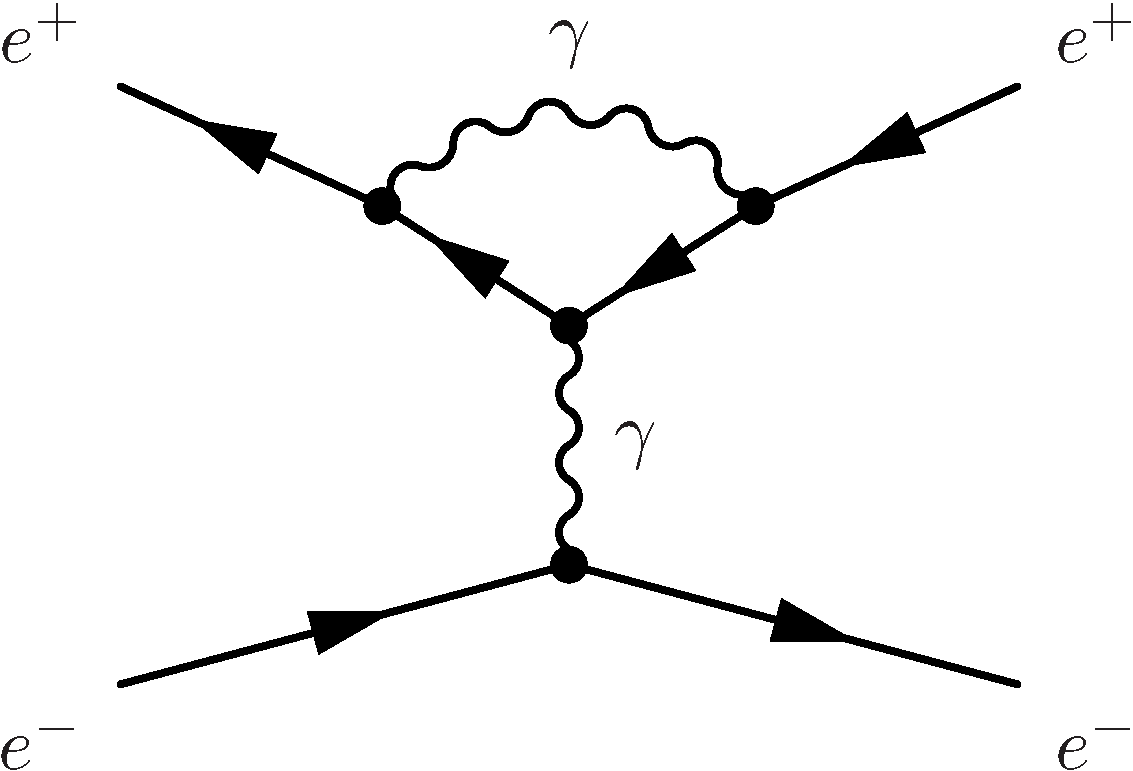
\includegraphics[width=.3\textwidth]{pics/vertex_correction}
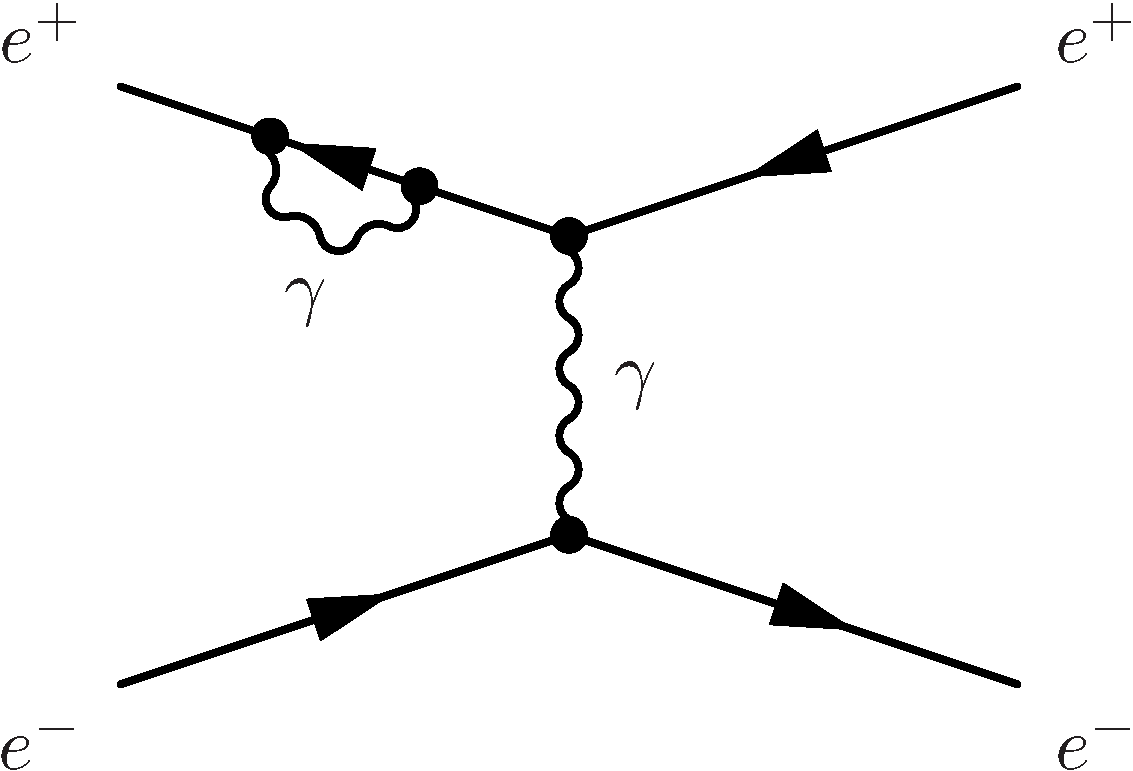
\includegraphics[width=.3\textwidth]{pics/self_energy}
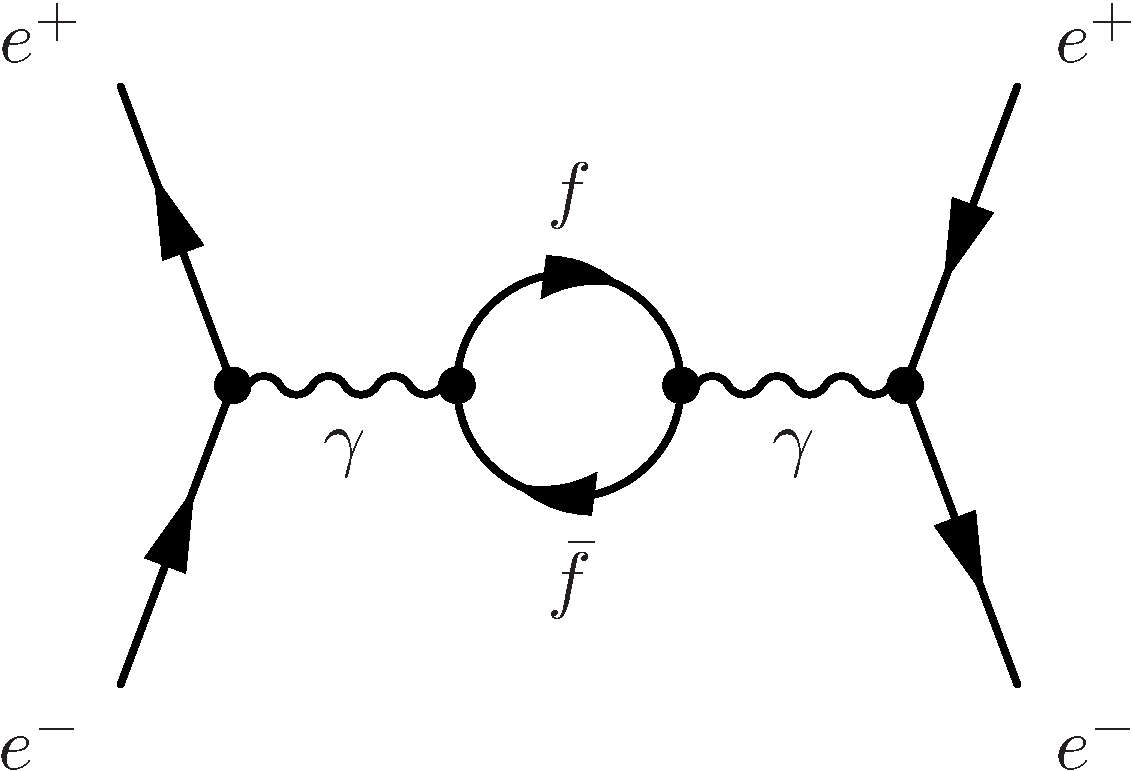
\includegraphics[width=.3\textwidth]{pics/mass_correction}
\end{center}
\caption{Radiative corrections at one loop in electron scattering. Time is directed horizontally. (left) The vertex correction for interaction strength. 
(middle) The self-energy correction for the electron. (right)   
The photon self-energy propagator correction.}
\label{fig:one_loop}
\end{figure}


\begin{figure}
\begin{center}
\includegraphics[width=.9\textwidth]{pics/loop8qed}
\end{center}
\caption{Example 8th order self-energy diagrams necessary for precision electroweak experiments \cite{loop8qed}.}
\label{fig:loop8qed}
\end{figure}

The perturbative expansion of the scattering matrix introduces momenta unconstrained by the in-going and out-going momentum
and must be integrated out in our calculation of a scattering amplitude (Figure \ref{fig:one_loop}). By construction  
these diagrams must be integrated up to infinite energies. This can lead to infinite matrix elements. 
Such a process is clearly unphysical, as its probability has no proper normalization. The
means of interpreting these infinite contributions to a matrix element is known as renormalization. The method of 
renormalization was a historical triumph of quantum field theory as a tool of describing high energy particle physics.
In the Wilsonian perspective of renormalization, an effective theory like the Standard Model would only integrate
over momentums below some finite energy scale where we expect the theory to no longer valid, the cut off scale $\Lambda$. This
scale has important consequences for the theory. All dimensionful parameters of the theory will be expressed in
terms of $\Lambda$ times constants which must be tuned against the cutoff. The level to which these constants must
be tuned to agree with measured values is known as the ``natural"-ness of the theory. 

\begin{figure}
\begin{center}
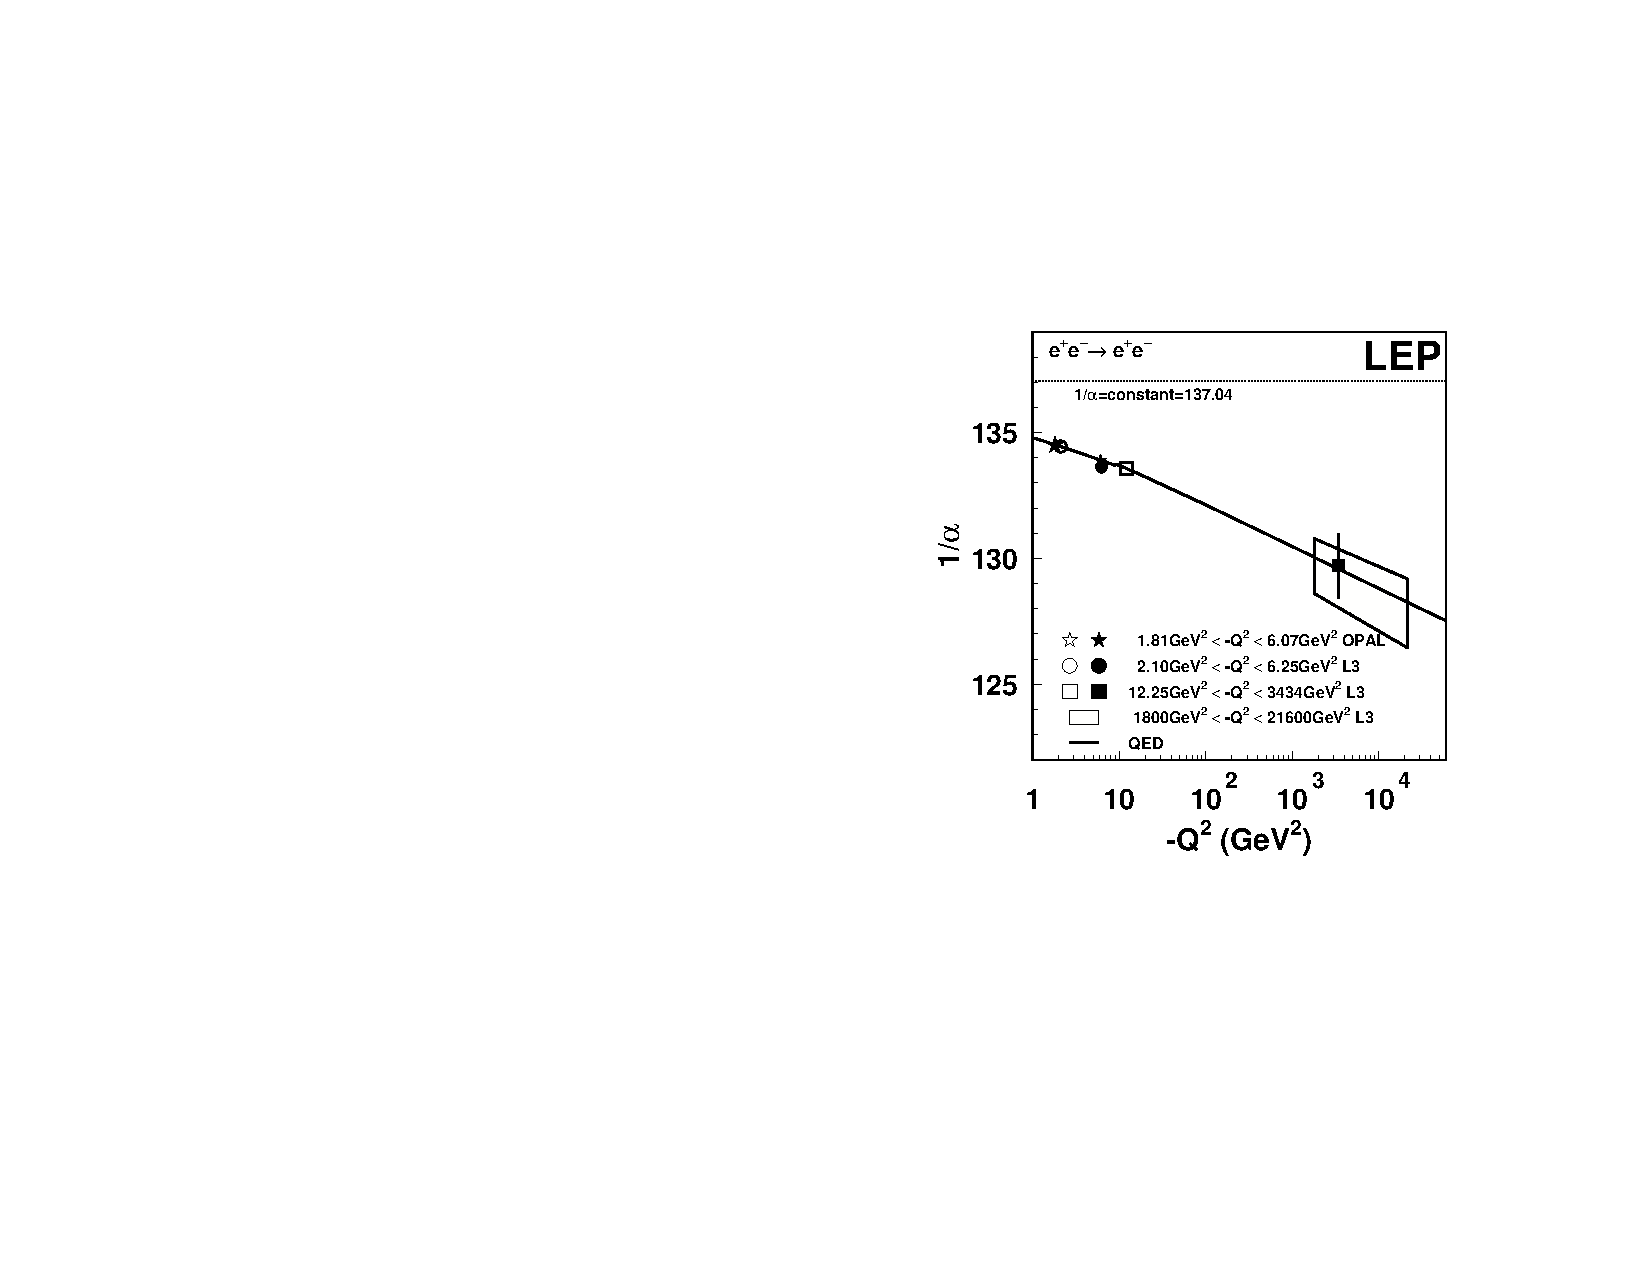
\includegraphics[width=.54\textwidth]{pics/alpha_qed}
\end{center}
\caption{The running of the electromagnetic coupling $\alpha$ as a function of the momentum transfer $Q^2$.}
\label{fig:running_coupling_qed}
\end{figure}

\begin{figure}
\begin{center}
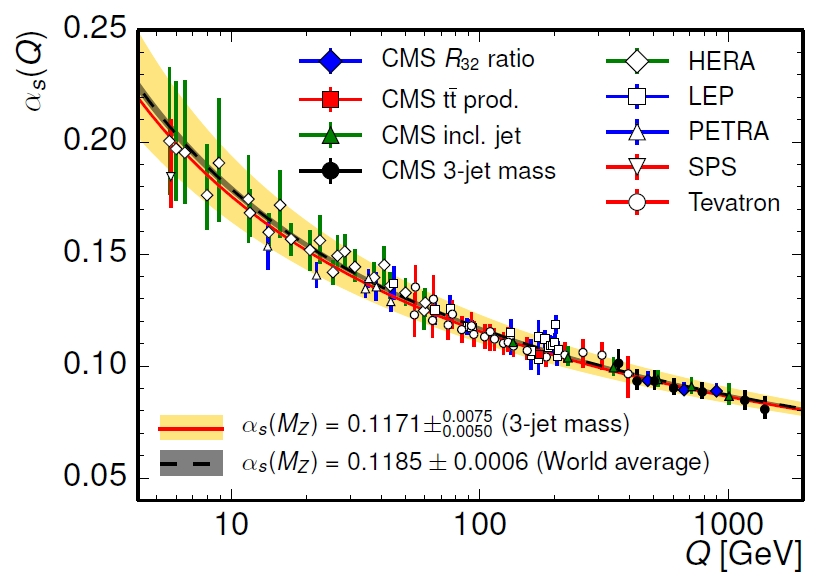
\includegraphics[width=.65\textwidth]{pics/alpha_s}
\end{center}
\caption{The running of the strong coupling constant $\alpha_s$ as a function of the momentum transfer $Q$.}
\label{fig:running_coupling_s}
\end{figure}


Examples of one loop diagrams are shown in Figure \ref{fig:one_loop}. These diagrams have important consequences on the
experimentally measured values of the parameters of the theory. The first diagram gives a correction to the electroweak coupling
strength and the electron magnetic moment. The second and third diagrams induce corrections to the electron and photon propagator,
respectively. An important consequence is on parameters of the theory. For instance, values of the coupling strength 
will effectively change or ``run'' with
the momentum transfer of the process $q^2$ . Historically, experiments
(Figures \ref{fig:running_coupling_qed} and \ref{fig:running_coupling_s}) have confirmed the $q^2$ dependence of the
 couplings $\alpha_s, \alpha$. Additionally, these loops will have contributions from all 
possible vertices in the Lagrangian, not just the flavors and families included in the in and 
out going states. Interestingly, the largest uncertainty in precision electroweak theory comes from hadronic loop contributions.

When dimensional analysis is performed on Lagrangian terms with mass dimension greater than 4, say $\frac{g}{5!}\phi^5$ 
a consequence of the action begin dimensionless is the coupling constant $g$ must have dimension $1/[M]$. As the only
mass scale in the theory is $\Lambda$,  
the coupling will scale as $1/ (c \Lambda)$ where $c$ is some dimensionless number. 
When the scales probed by the theory are small compared to cutoff $q^2/\Lambda^2 \rightarrow 0$
these terms are irrelevant in the theory. If the higher dimensional operators existed, we would only
see evidence when probing energies $q^2 \sim \Lambda^2$.  This would be evidence of new physics to 
be incorporated and a subsequent increase of the value of $\Lambda$ to where the new theory would break down. 

\begin{figure}
\begin{center}
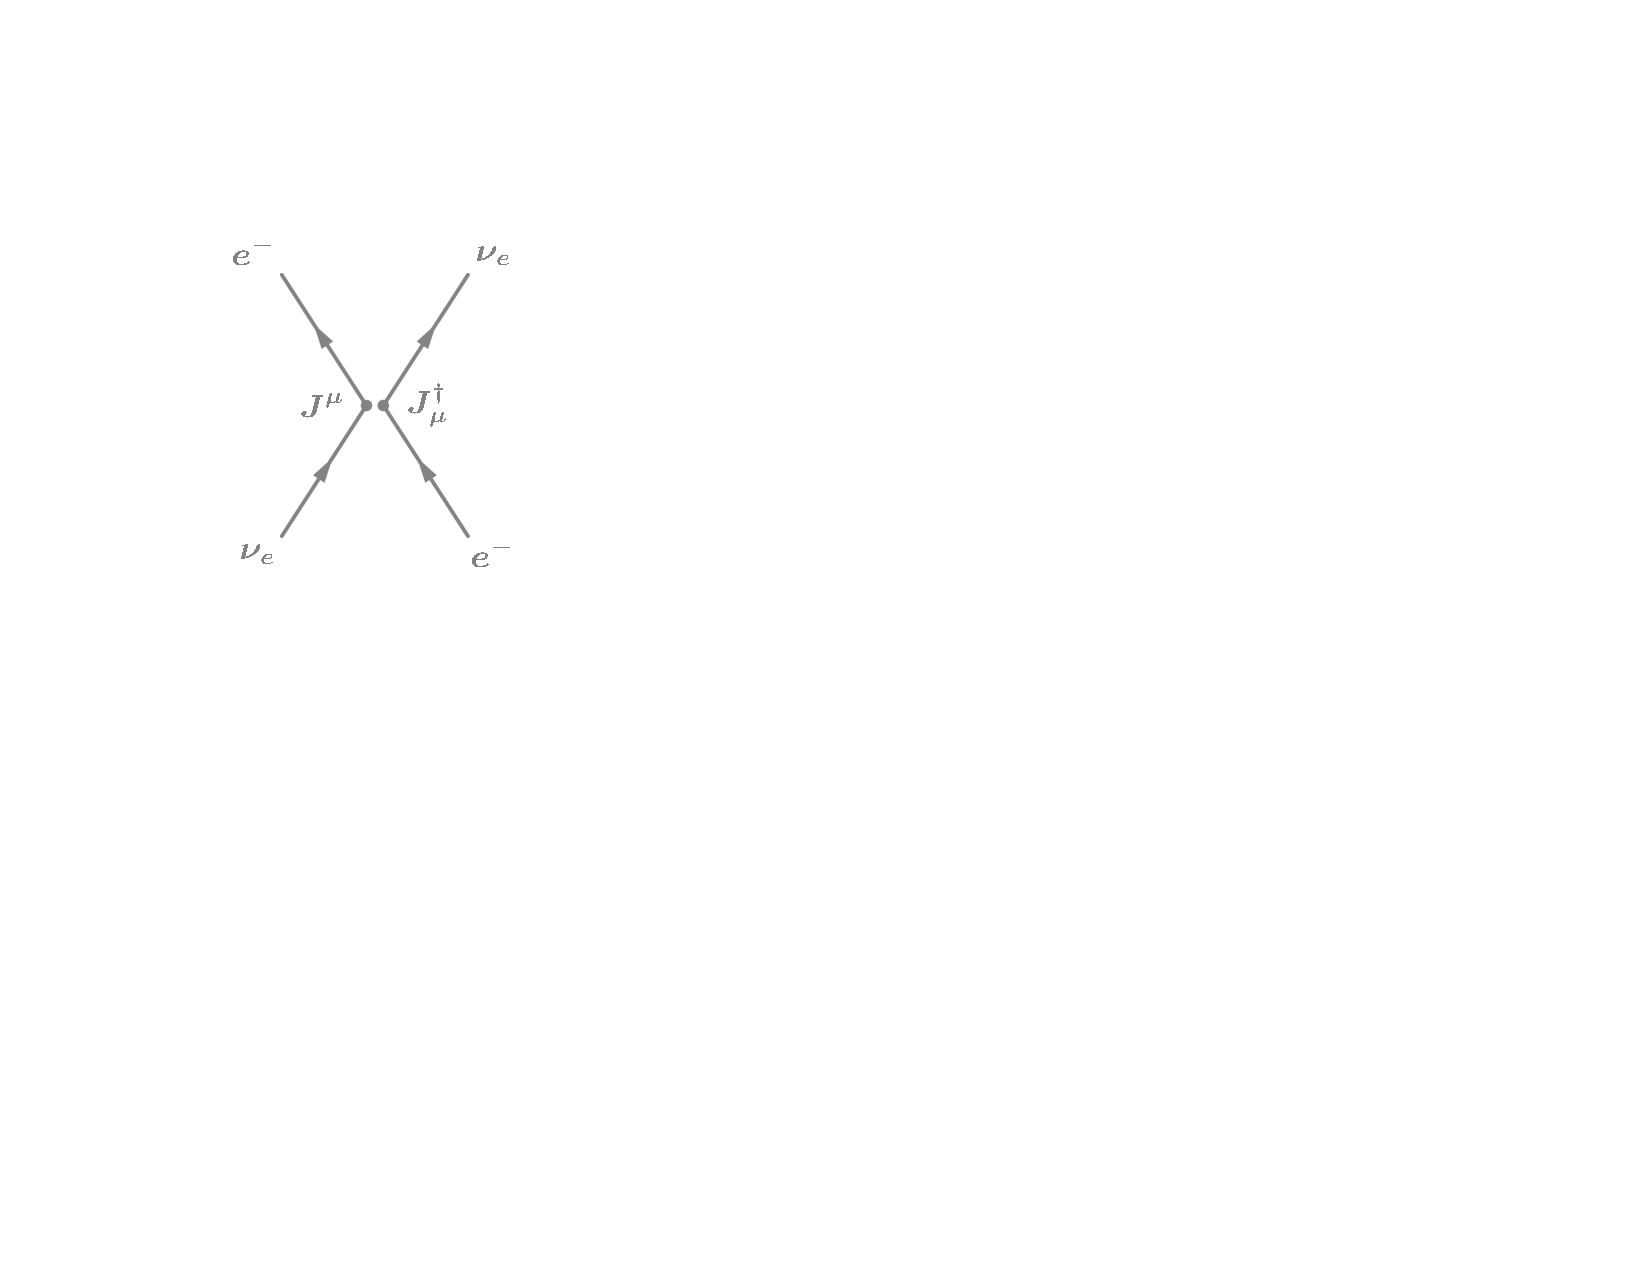
\includegraphics[width=.25\textwidth]{pics/fermi_theory}
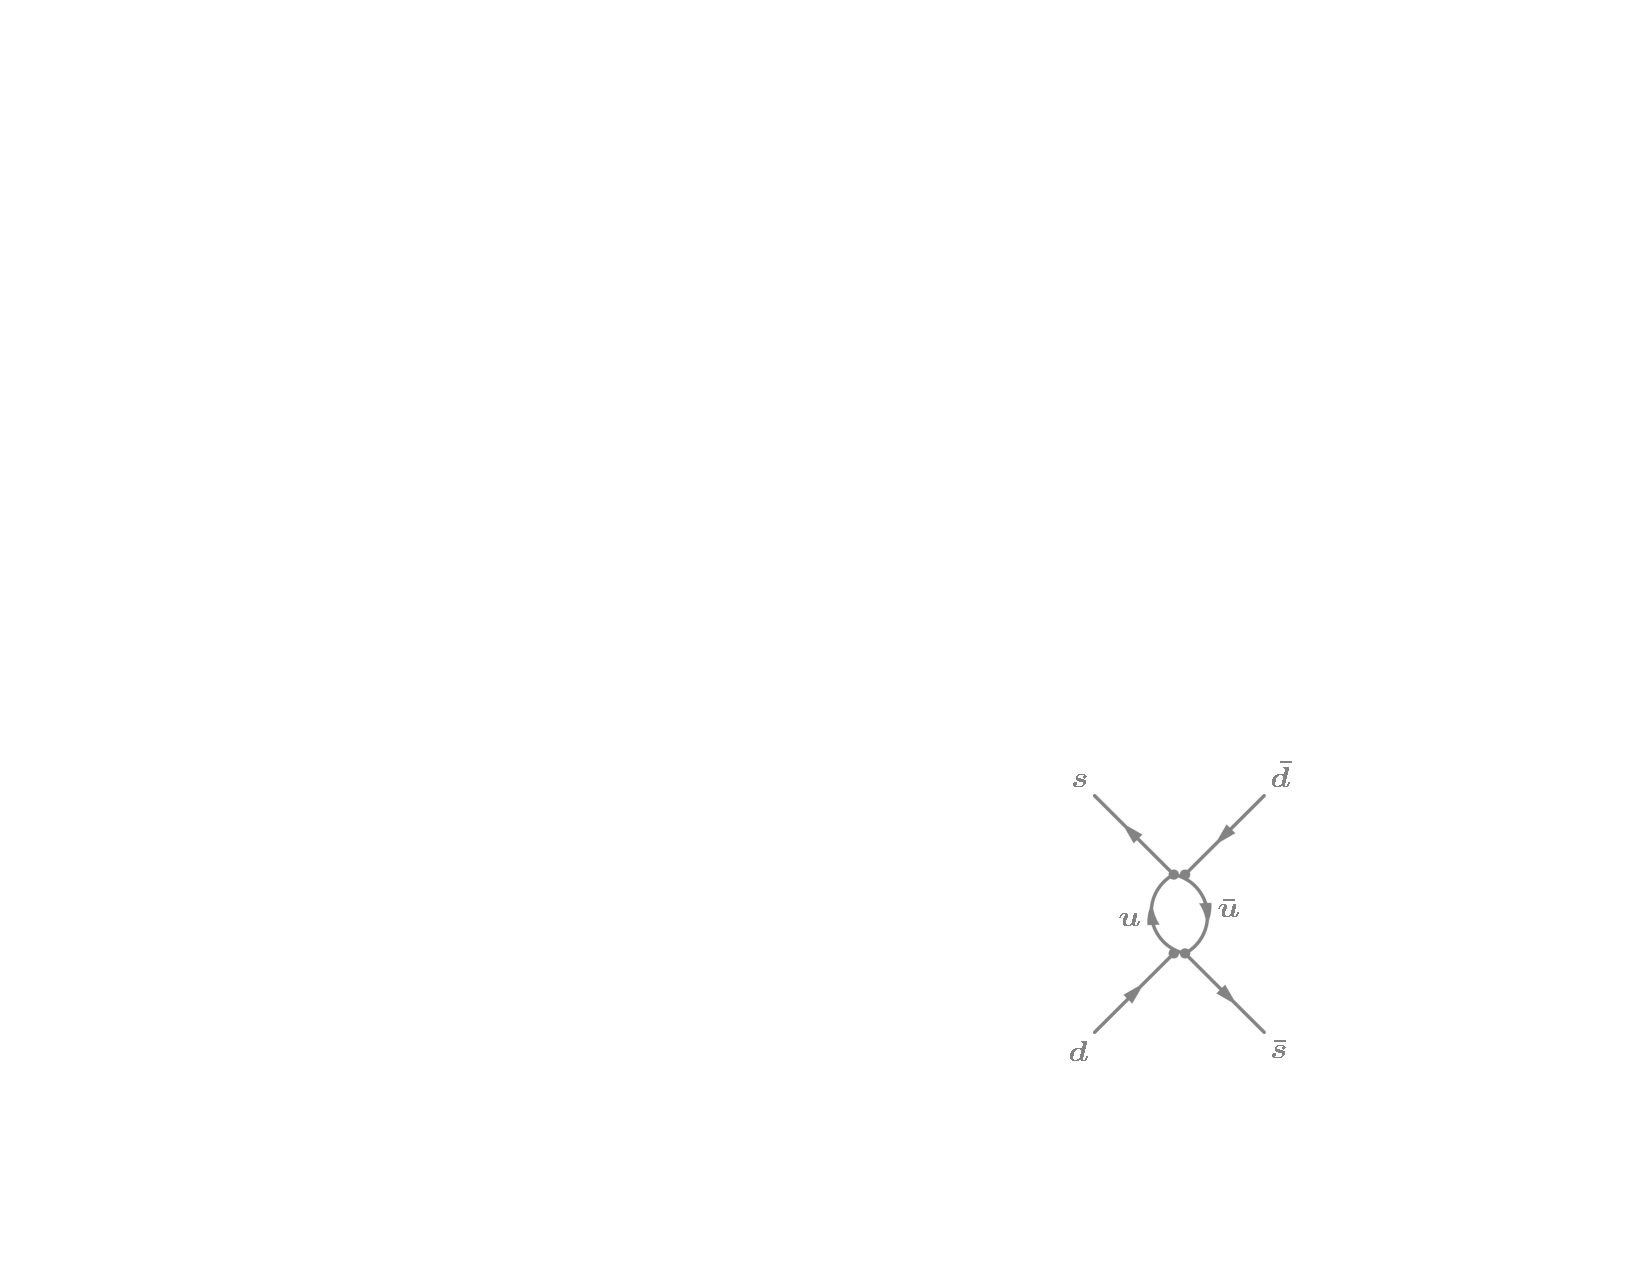
\includegraphics[width=.25\textwidth]{pics/fermi_diverge_ds}
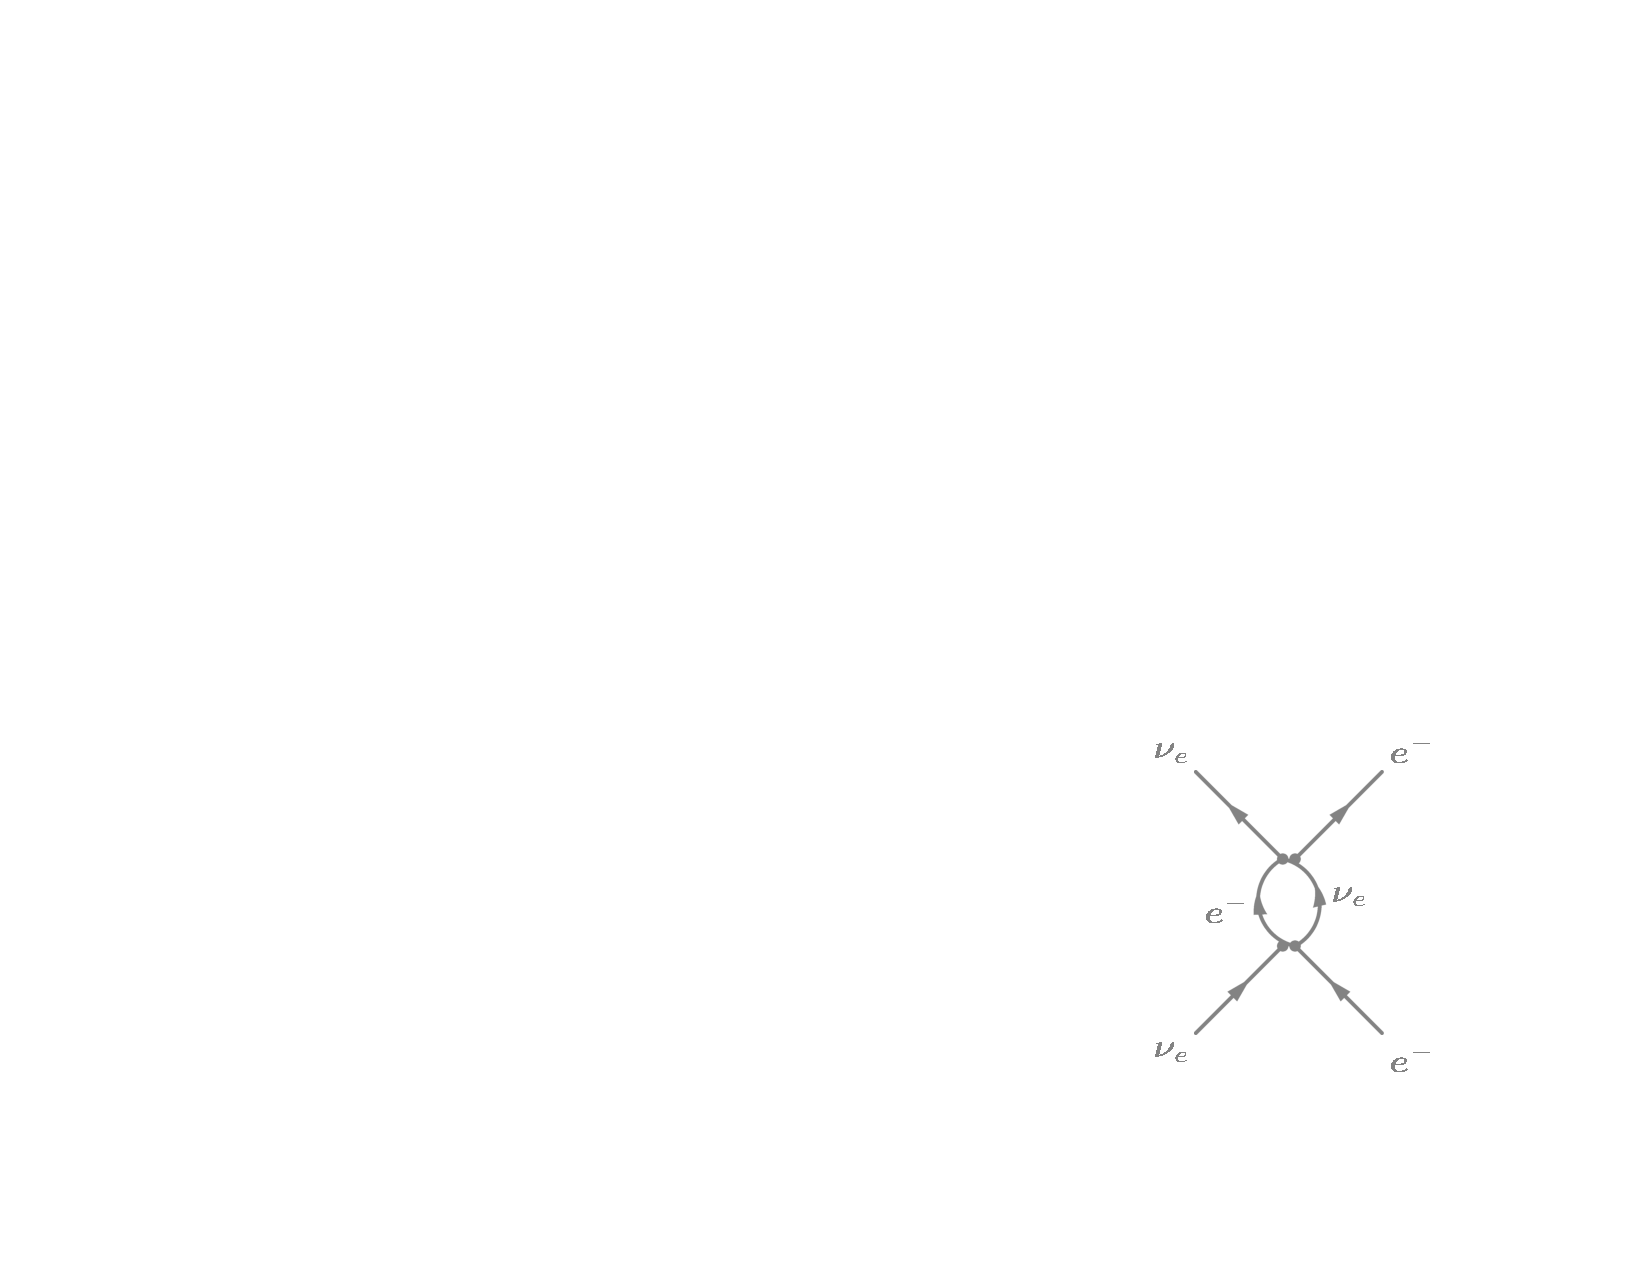
\includegraphics[width=.25\textwidth]{pics/fermi_divergence}
\end{center}
\caption{(left) The two current four fermi interaction describing electroweak processes. (center and right) Two divergent diagrams with caused by
an unconstrained momentum in the inner loop.}
\label{fig:fermi_divergence}
\end{figure}

As a concrete example, we consider the four point Fermi interaction which models electroweak theory as a contraction
 of hadronic and leptonic currents 
\begin{align*}
-\mathcal{L}  &= \frac{G_F}{\sqrt{2}} J^\dagger_\mu J^\mu  \text{ with } J_\mu = J^l_\mu + J^{had}_\mu\\
J_\mu^l &= \bar{e}^- \gamma_\mu (1- \gamma^5) \nu_e + \bar{\mu} \gamma_\mu (1- \gamma^5) \nu_\mu \\
J_\mu^{had} &= \bar{u} \gamma_\mu (1- \gamma^5) d'
\end{align*}
These diagrams are capable of describing a variety of processes correctly at tree level\cite{langacker}:
\begin{itemize}
\item Neutron $\beta$ decay: $n\rightarrow p e^-\bar{\nu}_e$
\item $\mu,\tau$ decay: $\mu^- \rightarrow e^- \bar{\nu}_e \nu_\mu$ and $\tau\rightarrow \mu^- \bar{\nu}_\mu \nu_\tau$ 
\item $\pi,K$ decay: $\pi^+ \rightarrow \mu^+ \nu_\mu$ 
\item heavy quark decays: $c \rightarrow s e^+ \nu_e$ and  $b \rightarrow c \mu^- \bar{\nu}_\mu$ 
\end{itemize}
While the model is successful at tree level, the theory has quadratically divergent diagrams  $O(\Lambda^2)$ (Figure \ref{fig:fermi_divergence}) at one loop.
\begin{align*}
\int d^4k \left ( \frac{k_\mu \gamma^\mu}{k^2} \right ) \left ( \frac{k_\mu \gamma^\mu}{k^2} \right ) \sim \int dk k  \sim \Lambda^2 
\end{align*}
\begin{figure}
\begin{center}
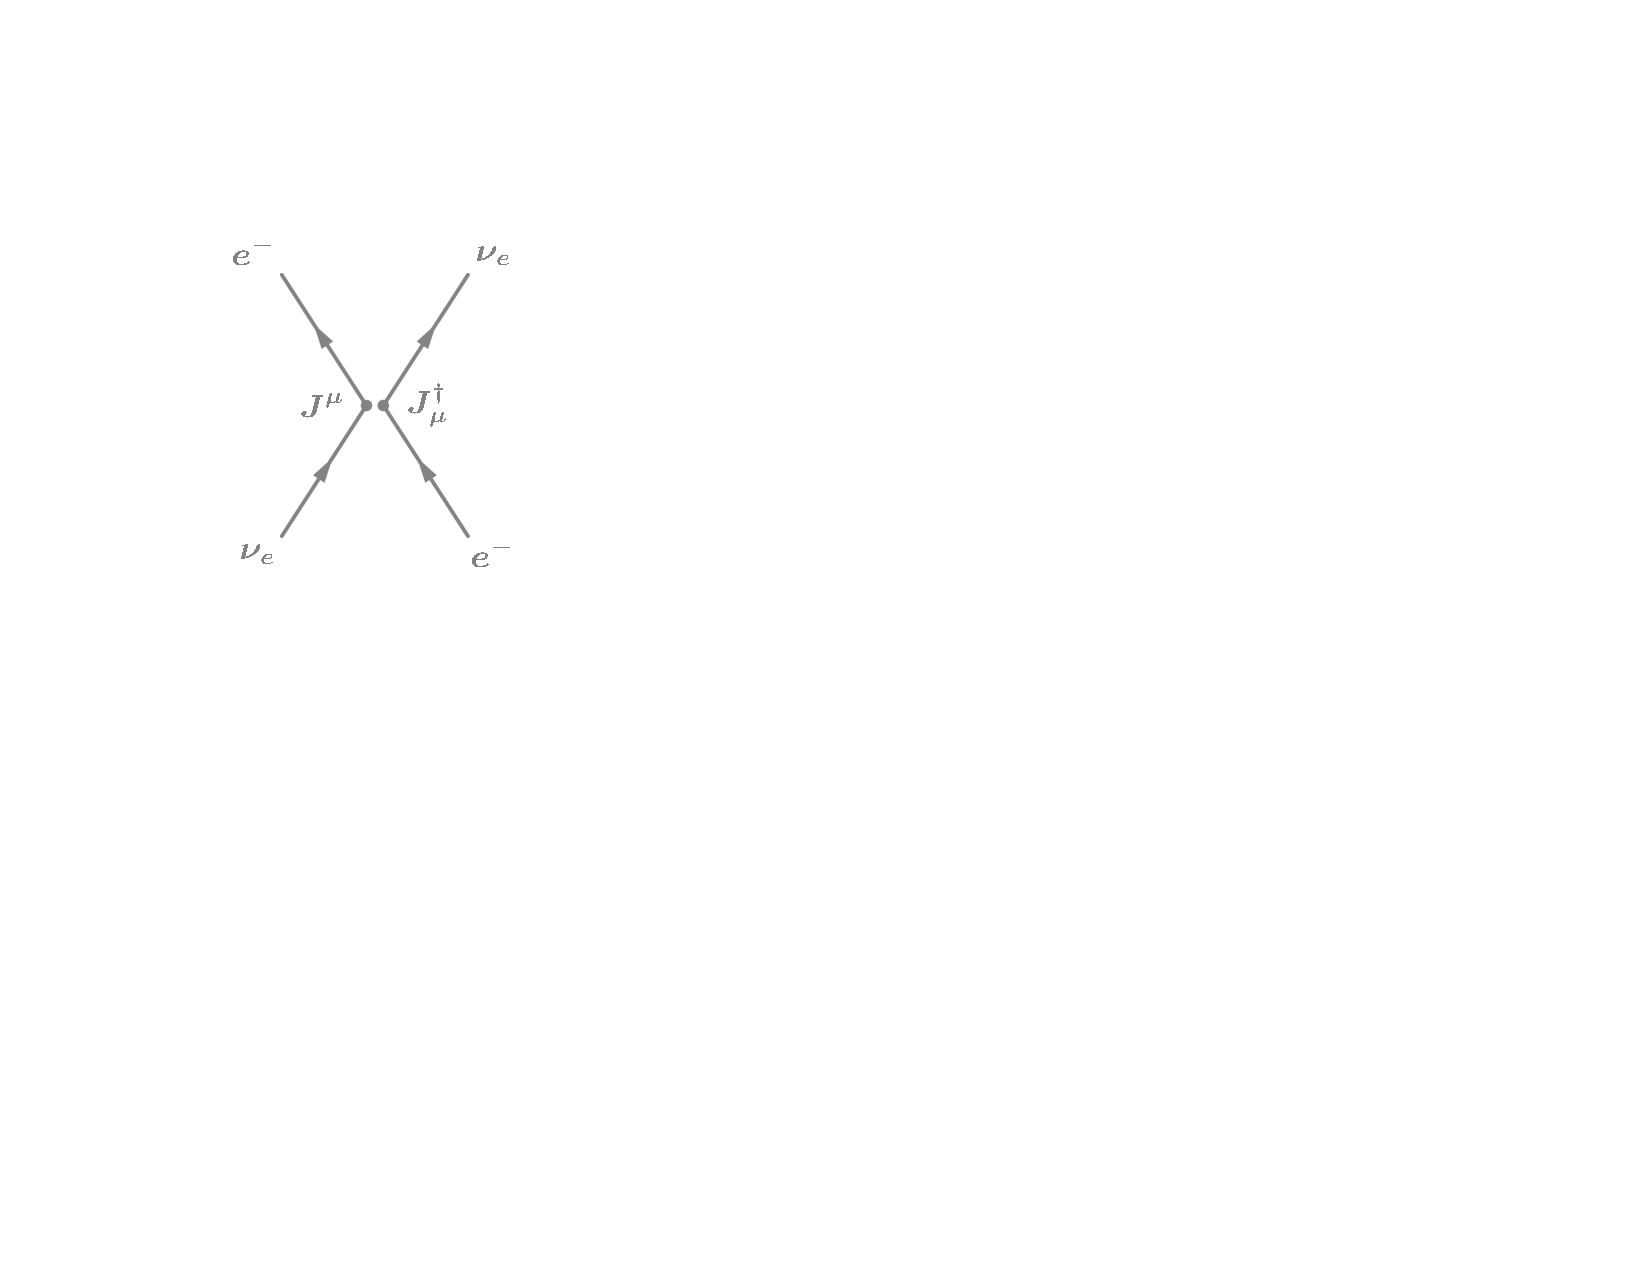
\includegraphics[width=.25\textwidth]{pics/fermi_theory}
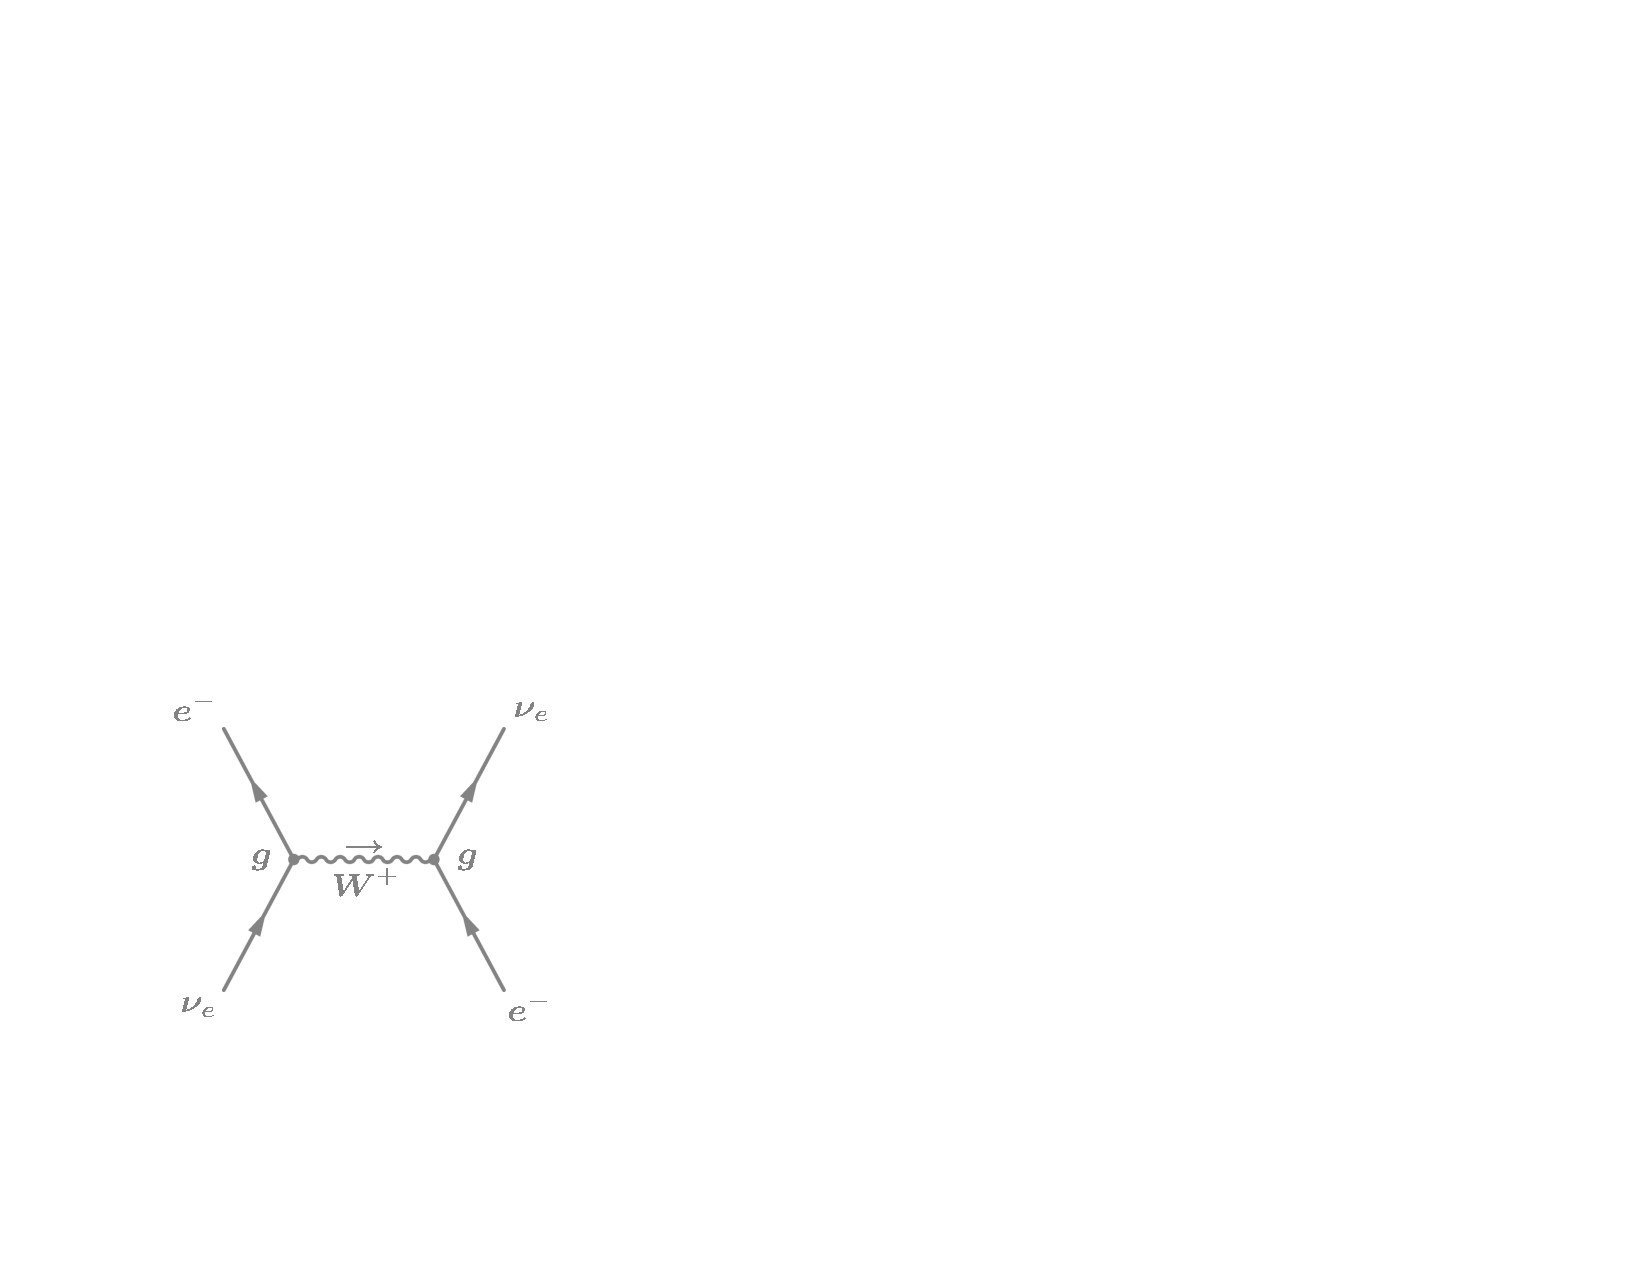
\includegraphics[width=.35\textwidth]{pics/int_vec_boson}
\end{center}
\caption{ The four fermi theory (left) for the weak interaction in
 terms of currents $J^\mu$  is realized in the Standard Model through a three point function including intermediate vector boson propagator (right).}
\label{fig:int_vec_boson}
\end{figure}
Since a fermion has $[\psi] \sim [M]^{3/2}$ the coupling $G_F$ must have dimension $[M]^{-2}$ and is therefore
non-renormalizable. New physics at the electroweak scale was needed to complete the theory in the ultraviolet (UV). Today, 
we know these diagrams needed an intermediate vector boson (Figure \ref{fig:int_vec_boson}) to be UV complete. The $[M]^{-2}$ dependence
of the $G_F$ was in fact due to the $W$'s propagating mass:
\begin{align*}
G_F = \frac{\sqrt{2}}{8} \frac{g_W^2}{m_W^2} \text{ with } m_W\approx 80 \text{ GeV and } g_W = 0.65
\end{align*}

\section{Supersymmetry (SUSY)}

The general discussion of SUSY at the level of experimental particle
 physics typically begins by positing 
that SUSY is a symmetry of particles. For every scalar particle, it posits a fermionic partner (and vice versa). 
This is experimentally relevant to designing searches for new particles. As the super partners 
of Standard Model particles have not yet been discovered it stands to reason they must be much heavier than their partners implying 
Supersymmetry is a broken symmetry. From loop corrections to Standard Model Feynman diagrams, we know
that the mass of these partners, should they exist in nature,
will determine the level of tuning required in the new theory.

It is less often mentioned that the theory of Supersymmetry 
posits something about the nature of the space-time.  Nature exhibiting Supersymmetry would arise
through an expansion of the fundamental coordinates of spacetime to
include components that are neither space nor time. In this section, we will discuss the elementary
 aspects of how Supersymmetry \cite{susybook} extends the usual quantum field theory 
discussed previously in this section. The goal is to have a basic understanding of the theory that has served as a major
motivation for the Large Hadron Collider.

To begin our discussion, we first need to review Lorentz transformations in terms of $SL(2,\mathbb{C})$
(read special linear group of order 2 with complex entries).  This group is convenient for 
expressing Lorentz transformations of a 4-vector $x^\mu$ by considering transformations on $\tilde{x} = x_\mu \sigma^\mu$ 
where $\sigma^\mu = (1,\vec \sigma)$ and $\bar{\sigma}^\mu = (1,-\vec \sigma)$. $\vec{\sigma}$ are 
the usual Pauli spin matricies. The transformation $\tilde x \rightarrow N \tilde x N^\dagger$ preserves
$det(\tilde{x}) = x_0^2 - \vec{x}^2$. The map between $\Lambda \in SO(3,1)$ the Lorentz group 
transformations
and $N \in SL(2,\mathbb{C})$ has a redundancy caused by the 2 to 1 mapping of $N= \pm 1$ to the identity. Explicitly 
we can write $\Lambda^\mu{}_\nu$ in terms of the transformation $N$ as:
\begin{align*}
\Lambda^\mu{}_\nu = \frac{1}{2} Tr \left \{ \bar{\sigma}^\mu N \sigma_\nu N^\dagger \right \}
\end{align*}
The representations of $SL(2,\mathbb{C})$ act on Weyl spinors which 
have an spinor index $\alpha=1,2$ corresponding to the two dimensions of the transformation. 
The left handed Weyl spinors transform under $N$ as:
\begin{align*}
\psi_\alpha ' = N_{\alpha}{}^\beta \psi_\beta 
\end{align*}
The right handed Weyl spinors transform under the conjugate representation. Indices which transform under the conjugate representation are denoted by a dot $\dot\alpha$
\begin{align*}
\bar{\chi}_{\dot \alpha}' =  N_{\dot \alpha}^*{}^{\dot \beta} \bar{\chi}_{\dot \beta}
\end{align*}
Just as the momentum operator $P^\mu$ and the generalized angular momentum operator $M^{\mu\nu}$ served 
as the generators of Poincar\'{e} lie group algebra, we have new Weyl spinor generators $Q_{\alpha}^A$
 and $\bar{Q}_{\dot{\alpha}}^A$ where $A=1,\ldots, \mathcal{N}$ indexes the number of super symmetries 
in the theory $\mathcal{N}$. A theory with $\mathcal{N}$ The Weyl spinors transform under the $SL(2, \mathbb{C})$ generators
$\sigma^{\mu\nu}_\alpha{}^{\beta} = \frac{i}{4}(\sigma^\mu \bar{\sigma}^\nu - \sigma^\nu\bar{\sigma}^\mu)_\alpha{}^\beta$
 and $\bar{\sigma}^{\mu\nu}_{\dot{\alpha}}{}^{\dot{\beta}} = \frac{i}{4}(\bar{\sigma}^\mu \sigma^\nu - \bar{\sigma}^\nu\sigma^\mu)^{\dot{\alpha}}{}_{\dot{\beta}}$ for the conjugate representation
\begin{align*}
Q_\alpha' = \exp \left ( \frac{i}{2} \omega_{\mu\nu} \sigma^{\mu\nu}{}_\alpha{}^\beta  \right ) Q_\beta
\end{align*}
By comparing the infinitesimal transformation between the Lorentz transformation and the $SL(2\mathbb{C})$ transformation we extract the commutation relations between $Q$ and $M^{\mu\nu}$:
\begin{align*}
[Q_\alpha, M^{\mu\nu}] = ( \sigma^{\mu\nu})_{\alpha}{}^{\beta} Q_\beta 
\end{align*}
From this we can determine $[Q, P^2] = 0$ which consequently shows us that multiplets of unbroken Supersymmetry
are degenerate in mass. Since we have not discovered these partners, we believe Supersymmetry is a broken symmetry. To understand how $Q$ acts on a state, we look at the commutation relations with the $z$ component spin operator $J_3$ which can be expressed in terms of $M^{\mu\nu}$ as $J_3 = \frac{1}{2}\epsilon_{3ij}M^{ij}$ for $i,j=1,2$. From this, we compute the commutator:
\begin{align*}
[Q_{\alpha}, J_3] &= \frac{1}{2}\epsilon_{3ij}[Q_\alpha, M^{ij}] = \frac{1}{2}\epsilon_{3ij} \left ( \frac{i}{4} [\sigma^j, \sigma^i] \right )_\alpha{}^\beta Q_\beta\\
&= -\frac{1}{4}(\epsilon_{3ij} \epsilon_{ji3} \sigma_3)_\alpha{}^\beta Q_\beta = -\frac{1}{2}(\sigma_3)_\alpha{}^\beta Q_\beta 
\end{align*}
The individual relations for the spinors are $[Q_1,J_3] = -\frac{1}{2}Q_1$ and $[Q_2, J_3] = \frac{1}{2} Q_2$.
That is to say, the Supersymmetry generators raise or lower the spin of a particle by $1/2$. This is important. The SUSY generators  
have the effect of interchanging fermionic and bosonic states!

From the structure of the indices we can also determine the anti-commutation relations between the
 generators up to a constant $c$ which is set to 2. 
\begin{align*}
\left \{ Q_\alpha, \bar{Q}_{\dot{\beta}}\right \} = c( \sigma^\mu)_{\alpha \dot{\beta}} P_\mu  = 2( \sigma^\mu)_{\alpha \dot{\beta}} P_\mu 
\end{align*}
here we see the two symmetry transformations together generate a translation in spacetime. This relation is suggestive that we should
 consider Supersymmetry a symmetry of spacetime. A complete super-Poincar\'{e} transformation (Lorentz transformations + translations + Supersymmetry transformations) is written in terms of the generators as:
\begin{align*}
g = \exp \left ( i ( \omega^{\mu\nu} M_{\mu\nu}  + a^\mu P_\mu + \theta^\alpha Q_\alpha + \bar{\theta}_{\dot{\alpha}}\bar{Q}^{\dot{\alpha}}) \right )
\end{align*}
where $\theta^\alpha$ and $\bar{\theta}_{\dot{\beta}}$ are spinors of anti-commuting Grassmann numbers
 which square to zero. In this way, $\theta^\alpha$ and $\theta_{\dot{\beta}}$ are like differential one 
forms $dx$ that only exist at linear order. When reading supersymmetric Lagrangians, which have explicit 
dependance on the $\theta$ and $\bar{\theta}$ spinors, it is important to understand the suppressed index structure. Although the 
individual Grassmann components of the spinor square to zero, the spinor terms will appear at second order as mixed components. 
\begin{align*}
\theta\theta &= \theta^\alpha \theta_\alpha = \epsilon^{\alpha\beta} \theta_\beta \theta_\alpha =  \theta_2 \theta_1 - \theta_1 \theta_2 = 2 \theta_2 \theta_1 \\
\bar\theta\bar{\theta} &= \bar{\theta}_{\dot{\alpha}} \bar{\theta}^{\dot{\alpha}} = (\theta_{\dot{\alpha}})^* (\theta^{\dot{\alpha}})^* = \theta_1^* \theta_2^* - \theta_2^* \theta_1^* = 2 \theta_1^* \theta_2^*
\end{align*}
The spinor indices between fermionic fields and $\theta$ are also suppressed $\theta\psi = \theta^\alpha \psi_\alpha$. 
Because $\theta_1^2=\theta_2^2=0$, there are no cubed spinor terms of the form $(\theta\theta)\theta\psi$ terms as all terms would be
at least order 2 in the components. It is also possible to formulate superspace in terms of Dirac matrices as a single component rather than two, however the majority of literature takes the Weyl spinor approach.

Now that we understand index structure, we can write the most general chiral super field as an expansion in the superspace coordinates as:
\begin{align*}
\Phi(x^\mu, \theta^\alpha, \bar{\theta}^{\dot{\alpha}}) = &\varphi(x) + \sqrt{2} \theta \psi(x) + \theta \theta F(x) + i \theta \sigma^\mu \bar{\theta} \partial_\mu \varphi(x) - \frac{i}{\sqrt{2} } (\theta\theta) \partial_\mu \psi(x) \sigma^\mu \bar{\theta}\\
& - \frac{1}{4}( \theta \theta ) (\bar{\theta} \bar{\theta} ) \partial_\mu \partial^\mu \varphi(x)
\end{align*}
Here $\sigma^\mu = (1, \vec \sigma)$. The field has 4 bosonic components ($\varphi$ and $F$) and 4 fermionic components ($\psi_\alpha$ i.e. one for each coordinate  $\theta_a$ and $\bar{\theta}_a$ ). When a super-translation is
 applied to the field, the individual coefficients of the super-coordinates will 
will transform into each other. However, it is possible to greatly reduce reduce therms with a transformation of variables $y^\mu = x^\mu + i \theta \sigma^\mu \bar{\theta}$. In these coordinates, the field appears only as a function of $\theta$.
\begin{align*}
\Phi(y^\mu, \theta^\alpha) = \varphi(y^\mu) + \sqrt{2} \theta \psi(y^\mu) + \theta \theta F(y^\mu) 
\end{align*}
$\varphi$ represents  the scalar components of the theory (squarks, sleptons, the Higgs) and $\psi$ the fermionic 
fields (quarks, leptons, and higgsinos). 

As for vector super-fields, the most general vector super-field expression is much longer:
\begin{align*}
V(x,\theta, \bar{\theta}) = &C(x) + i\theta \chi(x) - i \bar{\theta} \bar{\chi}(x)\\
&+ \frac{i}{2} \theta\theta (M(x) + iN(x)) - \frac{i}{2} \bar\theta \bar \theta (M(x)) \\
&- i N(x) + \theta\sigma^\mu \bar\theta V_\mu(x) + 
i \theta \theta \bar{\theta} \left ( -i \bar \lambda (x) + \frac{i}{2} \bar{\sigma}^\mu \partial_\mu \chi (x) \right)  \\
&-i \bar \theta \bar \theta \theta \left ( i \lambda (x) - \frac{i}{2} \sigma^\mu \partial_\mu \bar \chi (x) \right) + \frac{1}{2} (\theta\theta)(\bar \theta \bar \theta) \left( D - \frac{1}{2} \partial_\mu \partial^\mu C \right) 
\end{align*}
This field has 8 bosonic components ($C,M,N,D,V_\mu$) and 8 fermionic components $(\chi_\alpha, \lambda_\alpha)$.  
It is possible to build a vector super-field from a chiral field $\Lambda$ via $i(\Lambda - \Lambda^\dagger)$. 
With this, we can define a transformation $V \rightarrow V - \frac{i}{2}(\Lambda - \Lambda^\dagger)$ inducing a gauge 
transformation $V_\mu \rightarrow V_\mu + \partial_\mu (Re[\varphi]) = V_\mu + \partial_\mu \alpha$ that allows us the freedom to gauge away a number of components. In the Wess-Zumino Gauge, the vector field we can set $C = \chi = M = N = 0$ yielding a significantly reduced form:
\begin{align*}
V_{WZ} (x,\phi,\bar \phi) = (\theta \sigma^\mu \bar \theta) V_\mu (x) + (\theta\theta)\bar \theta \bar \lambda (x) 
+ (\bar \theta \bar \theta) \theta \lambda (x) + \frac{1}{2} ( \theta \theta) (\bar \theta \bar \theta) D(x) 
\end{align*}
In this form, $V_\mu$ corresponds to the usual Standard Model gauge bosons ($\gamma, W^\pm, Z, g$). $\lambda,\bar \lambda$
are the gauginos and $D$ is an auxiliary field. 

The most generic Lagrangian $\mathcal{L}$ for a chiral super-field is written in terms of the Khaler potential $K$ and the super potential $W$ as 
\begin{align*}
K(\Phi,\Phi^\dagger) &= \Phi^\dagger \Phi   \\
W(\Phi) &= \alpha + \lambda \Phi + \frac{m}{2}\Phi^2 + \frac{g}{3}\Phi^3\\
\mathcal{L} &= K |_{D}  + ( W|_F + h.c.)
\end{align*}
where we have taken the $D$ auxiliary term of the Kahler potential and the $F$ auxiliary term of the super potential. Expanding the Kahler potential in terms of the components of the most general solution to the chiral
 super field $\Phi$ and collecting the $D$ term (the coefficient of $\theta^2\bar{\theta}^2$):
\begin{align*}
K &= K_1 + K_2 + K_3 + K_4 \\ 
K_1 &= -\frac{1}{4} \bar{\theta}^2 \theta^2 ( \partial_\mu \partial^\mu \varphi^*)\varphi - 
\frac{1}{4} (\partial_\mu \partial^\mu \varphi) \varphi^*  \\
K_2 &=  - i \bar{\theta} \bar{\psi} \theta^2 ( \partial_\mu \psi \sigma^\mu \bar{\theta})  +
i \bar{\theta}^2 ( \theta \sigma^\mu \partial_\mu \bar{\psi}) \theta \psi  \\
K_3 &= (\theta \sigma^\mu \bar{\theta}) (\theta \sigma_\nu \bar{\theta}) \partial_\mu \varphi \partial^\nu \varphi \\
K_4 &= \bar{\theta}^2 \theta^2 |F|^2 
\end{align*}
$K_1$ can be written as a $\frac{1}{2}(\partial_\mu \varphi)(\partial^\mu \varphi^*)$ plus a total derivative which contributes 
zero in the action. $K_4$ yields another factor $\frac{1}{2}(\partial_\mu \varphi)(\partial^\mu \varphi^*)$ after contracting the 
$\sigma$ terms. $K_2$ yields the massless Dirac equation $-i\psi\sigma^\mu \partial_\mu \bar\psi$ plus a non contributing total derivative. The final
constant term $|F|^2$ is relevant to how SUSY is broken. Impressively, the simple expression of the Khaler potential as
a product of the most general chiral super-field and its conjugate yields precisely the free kinetic terms for the scalar and fermionic
fields. 
\begin{align*}
K = (\partial_\mu \varphi)(\partial^\mu \varphi^*) -i\psi\sigma^\mu \partial_\mu \bar \psi + |F|^2 
\end{align*}

For the potential terms, the derivatives of the super potential are evaluated in an expansion about
 $\Psi = \varphi$ where $\frac{\partial W}{\partial \varphi}
  = \frac{\partial W}{\partial \Phi}|_{\varphi}$
\begin{align*}
W(\Phi) = W(\varphi) + (\Phi - \varphi) \frac{\partial W}{\partial \varphi} + \frac{1}{2}(\Phi - \varphi)^2
\frac{\partial^2 W}{\partial \varphi^2}
\end{align*}
Evaluating the expansion at its $F$ term:
\begin{align*}
W(\varphi)|_F &= 0 \\
(\Phi - \varphi) \frac{\partial W}{\partial \varphi}|_F &= F(m\varphi +g \varphi^2) = -|m\varphi+g\varphi^2|^2\\
\frac{1}{2}(\Phi - \varphi)^2 \frac{\partial W}{\partial\varphi^2}|_F &= -\frac{1}{2}\psi^2(m+2g\varphi)
\end{align*}
Here we have made use of $-F = \frac{\partial W^*}{\partial \varphi^*}$ which can be obtained from minimal action. From the $F$ component of the Lagrangian $\mathcal{L}_{F} = |F|^2 + \frac{\partial W}{\partial \varphi}F + \frac{\partial W^*}{\partial \varphi^*}F^*$ 
we apply the minimal action principle and obtain $\frac{\delta S_{F}}{\delta F}
 = 0 \implies F^* + \frac{\partial W}{\partial \varphi}=0$ (the same is done for $F^*$.  
In this form, after adding the Hermitian conjugate of the potential term, the complete Lagrangian reads:
\begin{align*}
\mathcal{L} =& (\partial_\mu \varphi)(\partial^\mu \varphi^*) -i\psi\sigma^\mu \partial_\mu \bar \psi + |F|^2\\
&- | m\varphi + g\varphi^2 |^2  
- \psi^2 ( \frac{m}{2} + g \varphi) - \bar{\psi}^2 ( \frac{m}{2} + g\varphi^* ) + \partial^\mu \varphi \partial_\mu \varphi^*
\end{align*}
Now that we have the Lagrangian in terms of the super-field components, we can discuss why this construction is so attractive to the theoretical community. 

\subsection{The Miraculous Cancelation}

In this section, we would like to investigate the statement that supersymmetric top quarks
partners resolve the quadratic divergences in the Higgs mass corrections at one loop. 
In Supersymmetry, because the super potential is written only in terms the field
$\Phi$ the couplings between its scalar and fermionic components
 are sourced by the same coupling. As fermionic loops inherit a minus sign from fermionic statistics, this opens up the possibility of removing troubling 
 divergences. To check this, we will look at the corrections to the real components of the complex scalar field $\varphi$. This is based on material from the reference \cite{susybook}.

\begin{figure}
\begin{center}
\caption{The five 1 loop diagrams which correct the mass of the scalar particle $A$ at one loop \cite{susybook}. \label{fig:miraculous}}
\includegraphics[width=.65\textwidth]{pics/miraculous}
\end{center}
\end{figure}

The complex scalar field can then be expanded in terms of its real
 components $\varphi = (A+iB)/2$ yielding a Lagrangian
 $\mathcal{L}= \mathcal{L}_0 + \mathcal{L}_{int}$:
\begin{align*}
\mathcal{L}_0 = \frac{1}{2}\partial^\mu A \partial_\mu A - \frac{1}{2}m^2A^2 + \frac{1}{2}\partial^\mu B \partial_\mu B - \frac{1}{2}m^2 B^2 + \frac{1}{2}\bar{\psi}( i \gamma^\mu\partial_\mu - m) \psi \\
\mathcal{L}_{int} = \frac{mg}{\sqrt{2}}A(A^2 + B^2) - \frac{g^2}{4}(A^4+B^4+2A^2B^2) - \frac{g}{\sqrt{2}} \bar{\psi} (A-iB\gamma^5) \psi 
\end{align*}
From the interaction terms we see there are 2 quartic corrections to the propagating $A$ mass, one from the
$(g^2/4)A^4$ term and one from $(g^2/2)A^2B^2$. There are 2 scalar 3-point terms that contribute to the mass correction $(mg/\sqrt{2})A^3$ and $-(mg/\sqrt{2})AB^2$. Finally, and most importantly
there is a fermionic loop induced by $-(g\sqrt{2})\bar{\psi} A \psi$ with the same coupling $g$ that
will induce a cancelation. These corrections are summarized in Figure \ref{fig:miraculous}.

Diagrams (I) and (II) have similar form and are quadratically divergent. Adding the two diagrams:
\begin{align*}
4g^2 \int \frac{d^4k}{(2\pi)^4} \frac{1}{k^2 - m^2}
\end{align*} 
Diagram (III) has the same form as diagram (IV) and their contributions sum:
\begin{align*}
4g^2m^2 \int \frac{d^4k}{(2\pi)^4}\frac{1}{(k^2-m^2)((k-p)^2 - m^2)}
\end{align*}
Diagram (V) is more difficult to evaluate due to the gamma matrices in the fermionic loop. Ultimately, the integral expands into 3 terms:
\begin{align*}
&-\left(-\frac{ig}{\sqrt{2}}\right) 2 \int \frac{d^4k}{(2\pi)^4} Tr
 \left \{ \frac{i(\gamma^\mu k_\mu + m)}{k^2-m^2} \frac{i(\gamma^\mu k_\mu - \gamma^\mu p_\mu +m))}{(k-p)^2 - m^2}     \right \} \\
=& -2g^2 \left ( \int \frac{d^4k}{(2\pi)^4} \frac{1}{k^2-m^2} + \int \frac{d^4k}{(2\pi)^4} \frac{1}{(k-p)^2 -m^2} \right ) \\
 & -2g^2 \left (\int \frac{d^4k}{(2\pi)^4} \frac{4m^2 -p^2}{(k^2-m^2)((k-p)^2 -m^2)}  \right)
\end{align*}
The first term of (V) sums with diagrams (I) and (II) to:
\begin{align*}
2g^2 \int \frac{d^4k}{(2\pi)^4} \frac{1}{k^2 - m^2}
\end{align*}
The third term of (V) sums with diagrams (II) and (III):
\begin{align*}
-2g^2 \int  \frac{d^4k}{(2\pi)^4} \frac{2m^2 - p^2}{(k^2-m^2)((k-p)^2 - m^2)}
\end{align*}
The total correction is the sum of these three contributions is
\begin{align*}
2g^2 \left ( \int \frac{d^4k}{(2\pi)^4} \frac{1}{k^2-m^2} - \int \frac{d^4k}{(2\pi)^4} \frac{1}{(k-p)^2 -m^2} + \int \frac{d^4k}{(2\pi)^4 }\frac{p^2-2m}{(k^2-m^2)((k-p)^2 - m^2)} \right)
\end{align*}
The first two terms are quadratically divergent as $\int_\Lambda d^4k \frac{1}{k^2} \sim  \int_\Lambda dk k \sim \Lambda^2$. The third term is logarithmically divergent $\int_\Lambda d^4k/k^4\sim \int_\Lambda dk/k \sim \log(\Lambda)$. 

If the first two terms were evaluated  by dimensional regularization where
 \textit{all} momenta are integrated in d-dimensions (not just up to the scale $\Lambda$) the shift in the second term $k \rightarrow k-p$ would be inconsequential and the two terms would precisely cancel. However, if we take the Wilsonian
 point of view  and impose a strict cut off, the calculation can be performed by integrating the angular component of $k\cdot p$ on the three sphere. 
The ``miracle'' of this calculation is that the quadratic components 
between the first two terms cancel! The formulation of Supersymmetry imposes 
the same coupling constant for the super-symmetric partners (here $A$ and $\psi$). For this reason,
the quadratic divergences in their mass corrections will precisely cancel. When corrections 
are integrated to sum up the new physics $\Lambda$, say the
 gravitational scale $M_{pl}\sim 10^{18}$ GeV, the tuning required to keep the Higgs mass small is $\log(\Lambda)\sim 10^1$ rather than $10^{36}$! 
 Supersymmetry structurally preserves historical notions of naturalness.

In general, whether Supersymmetry exists or not, there are likely scalars which
couple to the Higgs with top-like couplings to cancel the quadratic divergences. The appeal of Supersymmetry is that these top like couplings come for free in the definition of the top super-field. 
Unfortunately, the Higgs remains the only fundamental scalar to be discovered at the LHC.


%% Combining the first two terms:
%% \begin{align*}
%% &2g^2 \left ( \int \frac{d^4k}{(2\pi)^4} \frac{(k^2-p^2) - (k-p)^2 + m^2}{(k^2-m^2)((k-p)^2 - m^2)}   - \int \frac{d^4k}{(2\pi)^4 }\frac{-2m^2 + p^2}{(k^2-m^2)((k-p)^2 - m^2)} \right)\\
%% =&2g^2 \left ( \int \frac{d^4k}{(2\pi)^4} \frac{-p^2}{(k^2-m^2)((k-p)^2 - m^2)}  + \int \frac{d^4k}{(2\pi)^4 }\frac{-2m^2 + p^2}{(k^2-m^2)((k-p)^2 - m^2)} \right)\\
%% =&2g^2  \int \frac{d^4k}{(2\pi)^4 }\frac{-2m^2 + p^2}{(k^2-m^2)((k-p)^2 - m^2)} 
%% \end{align*}

\subsection{The Minimally Supersymmetric Standard Model}

The Minimally Supersymmetric Standard Model (MSSM) is the minimally supersymmetric extension of the
Standard Model. This extension is minimal in the sense that it has as few particles as necessary to 
have a consistent theory and nothing more. As mentioned previously, each Standard Model particle
has a supersymmetric partner. The top quark has a stop quark partner and the electron has a selectron
partner. However, when experiments at the LHC design searches for super partners, the
numerous particles and names are not as straightforward to understand. Who is the standard model
partner of the chargino? Why are there multiple higgses and neutralinos? 
It is the goal of this sub-section to explain the particle content of the MSSM, specifically the source
of many neutralinos, charginos, and additional higgs bosons. This discussion is done 
in greater detail in the reference \cite{meike}.

\begin{table}[tb]
\caption{The chiral super field content of the MSSM. squarks, quarks, leptons, and slepton multiplets
have three families as in the standard model. Notably, the MSSM includes a second Higgs doublet to remove
non-gauge invariant anomalies.~\label{tab:mssmmatter}}
\begin{center}
\begin{tabular}{ccc}
\textbf{Superfield} & \textbf{Spin-0 Component} & \textbf{Spin-1/2 Component} \\
\hline
$Q$  & left squark $(\tilde{u}_L ~ \tilde{d}_L)$ & left  quarks $(u_L, d_L)$ \\
$u$ & right up squark $\tilde{u}_R^*$ & right quark $u_R$ \\
$d$ & right down squark $\tilde{d}_R^*$ & right down quark $u_R$ \\
$L$ & left slepton $(\tilde{\nu}~\tilde{e}_L)$ & left lepton $(\nu~e_L)$\\
$e$ & right slepton $\tilde{e}_R$ & right lepton $e_R$ \\
$H_u$ & up type higgs $(H_u^+ ~ H_u^0)$ & up type higgsino $(\tilde{H}_u^+ ~ \tilde{H}_u^0)$\\
$H_d$ & down type higgs $(H_d^0 ~ H_d^-)$ & down type higgsino $(\tilde{H}_d^+ ~ \tilde{H}_u^-)$\\
\end{tabular} 
\end{center}
\end{table}

\begin{table}[tb]
\caption{The vector super field content of the MSSM before EWSB. Correspondingly,
there are only super partners for the original gauge bosons in the unstable
 vacuum $\langle \phi \rangle =0$.~\label{tab:mssmbosons}}
\begin{center}
\begin{tabular}{cc}
\textbf{Spin-1/2 Component} & \textbf{Spin-1 Component} \\
\hline
gluino $\tilde{g}$ & gluon $g$\\
charged winos $\tilde{W}^{\pm}$, neutral wino $\tilde{W}$ & charged $W^\pm$, neutral $W$ \\
bino $\tilde{B}$ & $B$ boson 
\end{tabular} 
\end{center}
\end{table}

As discussed previously, a supersymmetric model is written in terms of chiral and vector super fields. 
The MSSM field content is summarized in Tables \ref{tab:mssmmatter} and \ref{tab:mssmbosons}. Notably
an additional Higgs multiplet has been included with opposite weak hyper charge $Y_{H_d}=-Y_{H_u}$ such that
the 1 loop three point gauge anomaly cancels. $H_u$ corresponds to the original Standard Model $SU(2)$ doublet. 
The three point anomaly is not gauge invariant due to the higgisinos in the Higgs chiral super field.
 The second doublet cancels this contribution. When electroweak symmetry breaking occurs, both
 higgses will take on a vacuum expectation value:
\begin{align*}
\langle H_u \rangle = \frac{1}{\sqrt{2}} \begin{pmatrix} 0  \\ \nu_u  \end{pmatrix} \text{ and } 
\langle H_d \rangle = \frac{1}{\sqrt{2}} \begin{pmatrix} \nu_d \\ 0  \end{pmatrix}
\end{align*}
where $\nu_u^2 + \nu_d^2 = \nu^2$ the Standard Model vacuum expectation value. Given this relation, we define the 
quantity $\tan{\beta} = \frac{\nu_u}{\nu_d}$ in terms of the right triangle with legs $\nu_u$ and $\nu_d$.
This is a free parameter of the theory and commonly scanned in tests of the MSSM. We believe
SUSY is a broken symmetry as the super parters have not been discovered, but there is no consensus
on how the symmetry is broken. To separate the discussion of how SUSY is broken and the consequences, 
certain ``soft'' terms are added to the Lagrangian with free parameters that are determined by how
the symmetry is broken. Specific to the Higgs potential the terms which explicitly break SUSY are
 $V_{\text{soft}} = m_{H_u}^2 H_u^2 + m_{H_d}^2 H_d^2 + (bH_uH_d  + h.c.)$. Combining this with the relevant
component of the Higgs potential  $\frac{1}{2} \sum_a g_a (\phi^*T^a\phi)^2$ where $T^a$ are the generators of the gauge
groups, we obtain the super symmetric Higgs potential:
\begin{align*}
V_{SUSY} &= (m_{H_u}^2 + |\mu|^2) H_u^2 + (m_{H_d}^2 + |\mu|^2) H_d^2 +  + \frac{1}{8}(g_1^2 + g_2^2)(H_u^2- H_d^2)^2 \\ 
&+ \frac{1}{2}g_2^2| H_u^+ H_d^{0*} + H_u^0H_d^{-*}|^2 + (b H_u^+H_d^- - bH_u^0 H_d^0 + h.c.) \\
V_{SM} &= \frac{1}{2}\mu^2 \phi^2 + \frac{1}{4}\lambda \phi^4
\end{align*}
From the Standard Model we set $m_Z^2 = (1/4)\nu^2(g_1^2 + g_2^2)$ and $m_W^2 = (1/4)\nu^2 g_2^2$. Expanding about the vacuum 
expectation values of $\langle H_u^0 \rangle$ and $\langle H_d^0 \rangle$ and diagonalizing the mass matrix, we arrive obtain five Higgs bosons $A,h,H^0,H^+,H^-$. $A$ is a CP odd Higgs. 
$h$ is the Standard Model Higgs. $H^0$ is a heavier CP even Higgs. $H^\pm$ are charged scalars. 
Counting our degrees of freedom we had two Higgs doublets with four complex components corresponding to eight degrees of freedom. 
Two degrees of freedom are lost during EWSB ($H_u^+$ and $H_d^-$) leaving six degrees of freedom. These correspond to the five Higgs bosons and the massless Goldstone boson.

As for the neutralinos the masses come from flavor mass mismatch between the binos, winos, and higginos. 
We list the relevant mass terms:
\begin{align*}
(-\frac{1}{2}M_1 \tilde{B} \tilde{B} - \frac{1}{2}M_2 \tilde{W}^0 \tilde{W}^0 + c.c) + (\mu \tilde{H}^0 \tilde{H}_d^0 + c.c.) - \sqrt{2}g \phi^*_i T^a_{ij}\psi_j \lambda^a
\end{align*}
Where $\psi_j = (\tilde{H}_u^0, \tilde{H}_d^0)$ and $\lambda^a = ( \tilde{B} , \tilde{W}^0)$ and $T^a$ are
the generators of the relavant gauge group. The mass matrix for the neutralinos is  $-(1/2)\psi^{T} M_{\tilde{\chi}^0} \psi + c.c$ :
\begin{align*}
m_{\tilde{\chi}^0} =
 \begin{pmatrix} 
M_1                  & 0                    & -g_1\frac{\nu_d}{2} & g_1 \frac{\nu_u}{2}  \\
  0                  & M_2                  & g_2\frac{\nu_d}{2}  & -g_2 \frac{\nu_u}{2} \\
 -g_1\frac{\nu_d}{2} & g_2 \frac{\nu_d}{2}  & 0                   & -\mu                 \\
 g_1\frac{\nu_u}{2}  & -g_2 \frac{\nu_u}{2} & -\mu                & 0 
\end{pmatrix} \text{ in the basis: } 
\begin{pmatrix} \tilde{B} \\ \tilde{W}^0 \\ \tilde{H}_u^0 \\ \tilde{H}_d^0 \end{pmatrix}
\end{align*}
This corresponds to four neutralinos that are combinations of the neutral pieces of the two pieces of the 
higgino doublets, the bino, and the neutral wino. For the charge mixing the relevant terms are:
\begin{align*}
-M_2\tilde{W}^+\tilde{W}^- - \mu \tilde{H}_u^+ \tilde{H}_d^- -  g_2 \nu_u \tilde{H}_u^+ \tilde{W}^- - g_2 
\nu_d \tilde{W}^+\tilde{H}_d^- + c.c.
\end{align*}
which amounts to a mass matrix of the form $-\frac{1}{2}\psi^{\pm T} M_{\tilde{\chi}^\pm} \psi^\pm + c.c.$:
\begin{align*}
M_{\tilde{\chi}}^\pm =
\begin{pmatrix} 
0        & 0        & M_2      & g_2\nu_d \\
0        & 0      & g_2\nu_u & \mu \\
M_2      & g_2\nu_u & 0        & 0   \\
g_2\nu_d & \mu      & 0        & 0 \end{pmatrix} \text{ in the basis: } 
\begin{pmatrix} \tilde{W}^+ \\ \tilde{H}_u^+ \\ \tilde{W}^- \\  \tilde{H}_d^- \end{pmatrix}
\end{align*}
The positive charginos are a mixed state of the + wino and the charged up type higgsino. The negative charginos are a mixed state of the + wino and the charged down type higgsino.

\section{Long-lived Signatures}

\subsection{Standard Model Particles with Long Lifetimes}

The Standard Model already includes a variety of common hadrons that can generate
displaced vertices (Table \ref{tab:mesons} and Table \ref{tab:baryons}). 
For example, $B^0 \rightarrow J/\psi K^{*0}$ with $K^{*0} \rightarrow K^+\pi^-$ 
generates a 4 charge particle vertex. 
Such a vertex is commonly utilized experimentally in 
b quark identification (b-tagging). Charge neutral Standard Model particles are of particular
 interest to identifying single displaced jets outside of the b-tagging lifetime regime. The most relevant states are those decaying to charged particles
 at a few centimeter proper lifetime, namely: $\Lambda^0$, $K_S^0$. 
These particles would have no charge particle leading 
to the primary collision vertex and a vertex
far outside B meson lifetimes. The most relevant of these processes being:
\begin{enumerate}
\item $K_s^0 \rightarrow \pi^+\pi^-$ 69\% of all $K_s^0$ decays 
\item $\Lambda^0 \rightarrow p \pi^-$ 64\% of all $\Lambda^0$ decays 
\end{enumerate}

\begin{figure}
\begin{center}
\includegraphics[width=.5\textwidth]{pics/kshorts}
\caption{The invariant mass of pairs of oppositely charged tracks in data and in simulation. Solid curves correspond to simulated
signal models which also contain displaced tracks, but do not share this resonant background as prominantly. \label{fig:kshorts}}
\end{center}
\end{figure}

Jets containing prompt decays as well as long-lived $K_s$ and $\Lambda^0$'s will contain tracks with large impact parameters. 
When a vertex is fit to such a jet, we expect small track multiplicity relative to 
massive $> 50$ GeV long-lived particles this analysis targets. Pairs of oppositely signed displaced tracks when vertexed together
generate a resonance in the invariant mass distribution as shown in Figure \ref{fig:kshorts}.


\begin{table}
\begin{center}
\begin{tabular}{cccccc}
\hline
\textbf{Name}  & \textbf{Content}                                    & \textbf{Particle}    & \textbf{mass} (MeV) & $\tau_{0}$ (sec)  & c$\tau$ (cm)         \\
\hline 
Pion & $u\bar{d}$                                  & $\pi^{\pm}$ & 139        & $2.6 \times 10^{-8}$       & $7.8 \times 10^{2}$  \\
\hline 
Kaon  & $u\bar{s}$                                 & $K^{\pm}$   & 497        & $     1.23 \times 10^{-8}$ & $3.7 \times 10^2$    \\
K Short  & $\frac{1}{\sqrt{2}}(d\bar{s} - s \bar{d})$ & $K^0_{s}$   & 497        & $0.896 \times 10^{-10}$    & 2.68                 \\
K Long  & $\frac{1}{\sqrt{2}}(d\bar{s} + s \bar{d})$ & $K^0_L$     & 497        & $5.1\times 10^{-8}$        & $1.5 \times 10^3$    \\
\hline
D & $c\bar{d}$                                 & $D^{\pm}$   & 1869       & $1 \times 10^{-12}$        & $3.0 \times 10^{-2}$ \\
\hline
B meson  & $u \bar{b}$                                & $B^{\pm}$   & 5279       & $1.6 \times 10^{-12}$      & $4.8 \times 10^{-2}$ \\
strange B  & $s\bar{b}$                                 & $B^{0}_s$   & 5366       & $1.5 \times 10^{-12}$      & $4.5 \times 10^{-2}$ \\
charmed B  & $c\bar{b}$                                 & $B^{0}_c$   & 6275       & $4.5\times 10^{-13}$       & $1.4 \times 10^{-2}$ \\
\end{tabular}
\end{center}
\caption{Mesons with Lifetimes greater than $10^{-2}$ cm} 
\label{tab:mesons}
\end{table}


\begin{table}
\begin{center}
\begin{tabular}{cccccc}
\textbf{Name}          & \textbf{Content} & \textbf{Particle}      & \textbf{mass} [MeV] &  $\tau_{0}$ [s] & $c\tau_{0}$ [cm] \\
\hline 
Lambda        & $uds$   & $\Lambda^0$   & 1115       & $2.6 \times 10^{-10}$    & 7.8                  \\
bottom Lambda & $udb$   & $\Lambda^0_b$ & 5620       & $1.4 \times 10^{-12}$    & $4.2 \times 10^{-2}$ \\
\hline
Sigma plus    & $uus$   & $\Sigma^{+}$  & 1189       & $8 \times 10^{-11}$      & 2.4                  \\
Sigma minus   & $dds$   & $\Sigma^{-}$  & 1197       & $1.4\times 10^{-10}$     & 4.2                  \\
\hline 
Xi zero       & $uss$   & $\Xi^0$       & 1314       & $4 \times 10^{-13}$      & $1.2 \times 10^{-2}$ \\
Xi minus      & $dss$   & $\Xi^-$       & 1321       & $1.6 \times 10^{-10}$    & 4.8                  \\
charmed Xi +  & $usc$   & $\Xi^{+}_c$   & 2467       & $4.42 \times 10^{-13}$   & $1.3 \times 10^{-2}$ \\
charmed Xi    & $dsc$   & $\Xi^0_c$     & 2471       & $1.12 \times 10^{-13}$   & $3.3 \times 10^{-2}$ \\
bottom Xi     & $dsb$   & $\Xi^-_b$     & 5792       & $1.56 \times 10^{-12}$   & $4.7 \times 10^{-2}$ \\
\hline
bottom Omega  & $ssb$   & $\Omega_b^-$  & 6054       & $1.13 \times 10^{-12}$   & $3.3 \times 10^{-2}$ \\
Omega minus   & $sss$   & $\Omega^-$    & 1672       & $8 \times 10^{-11}$      & 2.4                  \\
\end{tabular}
\end{center}
\caption{Baryons with Lifetimes greater than $10^{-2}$ cm} 
\label{tab:baryons}
\end{table}


Particles of a characteristic lifetime $\tau$ decay with a falling exponential distribution. For reference, 
a table summarizing the distribution is shown in Table
\ref{tab:lifetime}. As the BSM particles must decay with the detector used to identify them, it is important to note  that for proper
lifetimes 10 and 100 times the size of the relevant detector ($\sim$1 m), we would still expect
~10\% and 1\% of decays (respectively) to occur within the sensitive region of the detector.


\begin{table}
\begin{center}
\begin{tabular}{ccc}
Distance ($\lambda$) &  Probability of Decay  \\
\hline
0.01               & 1\%                        \\
0.1                & 9.5\%                      \\              
0.25               & 22\%                       \\            
0.5                & 39\%                       \\          
0.75               & 52\%                       \\        
1                  & 63\%                       \\      
1.5                & 77\%                       \\    
2                  & 86\%                       \\  
3                  & 95\%                       \\
5                  & 99.3\%                     \\
\end{tabular}
\end{center}
\caption{ A reference table for the cumulative probability for a particle of lifetime $\lambda$ to have decayed after a given
distance. Distance is in multiples of lambda.}
\label{tab:lifetime}
\end{table}


\subsection{Split SUSY and Naturalness at the LHC}

When motivating Supersymmetry with naturalness, 
it is important to note that the stability of the Higgs boson mass is not the only
 fine-tuning problem in particle physics. When the same argument is used to calculate
 the cosmological constant we arrive at cut off scale
 $\Lambda \geq m_{SUSY}^4$, where experimentally $\Lambda = 10^{-59}$ TeV$^4$.   
If we use the same SUSY scale $m_{SUSY} = 1$ TeV we have a new fine tuning problem of $10^{60}$!

As addressed by Arkani-Hamed and Dimopoulos \cite{nimalhc}, many theoretical approaches  have been
motivated by a natural explanation for the Higgs mass while separately seeking an  explanation
of the cosmological constant through some other mechanism.
Arkani-Hamed and Dimopoulos propose a reconsideration of naturalness, entertaining the idea that 
fine tuning could have a role to play in beyond the Standard Model physics.
Conceivably, both $\Lambda$ and $m_h$ fine tuning could be resolved by the same mechanism.  
This un-natural model was  further investigated by Giudice and Romanino \cite{splitsusy}
and dubbed ``Split Supersymmetry". 

Split SUSY assumes a much higher SUSY scale $m_{SUSY}^2 \gg 1$ TeV where all scalars
 (excluding the Higgs) become very heavy $O(m_{SUSY})$ and the lightest sparticles (higgsinos and gluinos) are kept at the TeV scale by requiring 
the lightest neutralino to be a good dark matter candidate. Because the scalars are so much heavier, the decay of gluinos through squarks is suppressed.
The characteristic signature of split Supersymmetry is thus long-lived gluinos \cite{hewett}; such processes 
with long lifetimes are rare in the Standard Model, particularly for particles with mass larger than the $m_{EW}$.

Following the discovery of the Higgs boson in July 2012, Arkani-Hamed et al. \cite{nimahiggs} investigated  the scalar super-partner mass scale for $m_h \approx 125$ GeV. %Shows $m_h$ vs. $M_{sc}$, the mass scale of the new scalars  for various values of $\tan \beta$. 
The most phenomenologically interesting point is the gluino lifetime given by:
\begin{align*}
c\tau_{\tilde{g}} \approx 10^{-5} m \left ( \frac{m_{\tilde{q}}}{\mbox{PeV}} \right )^4 \left( \frac{\mbox{TeV}}{m_{\tilde{g} }}\right)^5
\end{align*}
For massive gluinos still within the reach of the $\sqrt{s} = 13$ TeV LHC ($m_{\tilde{g}} \lesssim 3$ TeV) we would probe up to $m_{sq} \simeq 10^4$ TeV if the proper gluino lifetimes is on the order of the relevant detector ($c\tau_{\tilde{g}} < 1$ m).

As the Higgs at 125 GeV has been the only scalar discovered in the LHC's $\sqrt{s}= 7,8,$ and 13 TeV program, the natural SUSY parameter space has become more tightly constrained. 
If no new scalar super-partners are found soon, less natural scenarios like split SUSY would become even stronger candidates for BSM physics.
 CMS is well prepared for most, if not all, SUSY final states with prompt decays. Long-lived scenarios allow one to probe 
significantly higher energy scales if components of the theory are light enough to be probed at the LHC.
